\documentclass[twoside]{book}

% Packages required by doxygen
\usepackage{fixltx2e}
\usepackage{calc}
\usepackage{doxygen}
\usepackage[export]{adjustbox} % also loads graphicx
\usepackage{graphicx}
\usepackage[utf8]{inputenc}
\usepackage{makeidx}
\usepackage{multicol}
\usepackage{multirow}
\PassOptionsToPackage{warn}{textcomp}
\usepackage{textcomp}
\usepackage[nointegrals]{wasysym}
\usepackage[table]{xcolor}

% Font selection
\usepackage[T1]{fontenc}
\usepackage[scaled=.90]{helvet}
\usepackage{courier}
\usepackage{amssymb}
\usepackage{sectsty}
\renewcommand{\familydefault}{\sfdefault}
\allsectionsfont{%
  \fontseries{bc}\selectfont%
  \color{darkgray}%
}
\renewcommand{\DoxyLabelFont}{%
  \fontseries{bc}\selectfont%
  \color{darkgray}%
}
\newcommand{\+}{\discretionary{\mbox{\scriptsize$\hookleftarrow$}}{}{}}

% Page & text layout
\usepackage{geometry}
\geometry{%
  a4paper,%
  top=2.5cm,%
  bottom=2.5cm,%
  left=2.5cm,%
  right=2.5cm%
}
\tolerance=750
\hfuzz=15pt
\hbadness=750
\setlength{\emergencystretch}{15pt}
\setlength{\parindent}{0cm}
\setlength{\parskip}{3ex plus 2ex minus 2ex}
\makeatletter
\renewcommand{\paragraph}{%
  \@startsection{paragraph}{4}{0ex}{-1.0ex}{1.0ex}{%
    \normalfont\normalsize\bfseries\SS@parafont%
  }%
}
\renewcommand{\subparagraph}{%
  \@startsection{subparagraph}{5}{0ex}{-1.0ex}{1.0ex}{%
    \normalfont\normalsize\bfseries\SS@subparafont%
  }%
}
\makeatother

% Headers & footers
\usepackage{fancyhdr}
\pagestyle{fancyplain}
\fancyhead[LE]{\fancyplain{}{\bfseries\thepage}}
\fancyhead[CE]{\fancyplain{}{}}
\fancyhead[RE]{\fancyplain{}{\bfseries\leftmark}}
\fancyhead[LO]{\fancyplain{}{\bfseries\rightmark}}
\fancyhead[CO]{\fancyplain{}{}}
\fancyhead[RO]{\fancyplain{}{\bfseries\thepage}}
\fancyfoot[LE]{\fancyplain{}{}}
\fancyfoot[CE]{\fancyplain{}{}}
\fancyfoot[RE]{\fancyplain{}{\bfseries\scriptsize Generated by Doxygen }}
\fancyfoot[LO]{\fancyplain{}{\bfseries\scriptsize Generated by Doxygen }}
\fancyfoot[CO]{\fancyplain{}{}}
\fancyfoot[RO]{\fancyplain{}{}}
\renewcommand{\footrulewidth}{0.4pt}
\renewcommand{\chaptermark}[1]{%
  \markboth{#1}{}%
}
\renewcommand{\sectionmark}[1]{%
  \markright{\thesection\ #1}%
}

% Indices & bibliography
\usepackage{natbib}
\usepackage[titles]{tocloft}
\setcounter{tocdepth}{3}
\setcounter{secnumdepth}{5}
\makeindex

% Hyperlinks (required, but should be loaded last)
\usepackage{ifpdf}
\ifpdf
  \usepackage[pdftex,pagebackref=true]{hyperref}
\else
  \usepackage[ps2pdf,pagebackref=true]{hyperref}
\fi
\hypersetup{%
  colorlinks=true,%
  linkcolor=blue,%
  citecolor=blue,%
  unicode%
}

% Custom commands
\newcommand{\clearemptydoublepage}{%
  \newpage{\pagestyle{empty}\cleardoublepage}%
}

\usepackage{caption}
\captionsetup{labelsep=space,justification=centering,font={bf},singlelinecheck=off,skip=4pt,position=top}

%===== C O N T E N T S =====

\begin{document}

% Titlepage & ToC
\hypersetup{pageanchor=false,
             bookmarksnumbered=true,
             pdfencoding=unicode
            }
\pagenumbering{alph}
\begin{titlepage}
\vspace*{7cm}
\begin{center}%
{\Large Gateware Libraries \\[1ex]\large Beta Release }\\
\vspace*{1cm}
{\large Generated by Doxygen 1.8.12}\\
\end{center}
\end{titlepage}
\clearemptydoublepage
\pagenumbering{roman}
\tableofcontents
\clearemptydoublepage
\pagenumbering{arabic}
\hypersetup{pageanchor=true}

%--- Begin generated contents ---
\chapter{Gateware Libraries}
\label{index}\hypertarget{index}{}\begin{DoxyCopyright}{Copyright}
Copyright (c) 2016 7th\+Gate Software .L\+LC 
\end{DoxyCopyright}
\begin{DoxyParagraph}{License\+:}
Gateware libraries are released under Creative Commons M\+IT lincense unless noted differently by the library. 
\end{DoxyParagraph}
\begin{DoxyVersion}{Version}
Beta Release
\end{DoxyVersion}
\hypertarget{index_API}{}\section{A\+P\+I\+Overview}\label{index_API}
Coming Soon\hypertarget{index_APIOverview}{}\subsection{G\+Log}\label{index_APIOverview}
Coming Soon\hypertarget{index_GLog}{}\subsection{G\+File}\label{index_GLog}
Coming Soon\hypertarget{index_GFile}{}\subsection{G\+Input}\label{index_GFile}
Coming Soon\hypertarget{index_GInput}{}\subsection{G\+Buffered\+Input}\label{index_GInput}
Coming Soon\hypertarget{index_Installation}{}\section{Installation}\label{index_Installation}
Coming Soon\hypertarget{index_Bug}{}\section{Reporting}\label{index_Bug}
Coming Soon 
\chapter{Namespace Index}
\section{Namespace List}
Here is a list of all documented namespaces with brief descriptions\+:\begin{DoxyCompactList}
\item\contentsline{section}{\mbox{\hyperlink{namespace_g_w}{GW}} \\*The core namespace to which all Gateware interfaces/structures/defines must belong }{\pageref{namespace_g_w}}{}
\item\contentsline{section}{\mbox{\hyperlink{namespace_g_w_1_1_a_u_d_i_o}{G\+W\+::\+A\+U\+D\+IO}} \\*The namespace to which all Gateware library interfaces must belong }{\pageref{namespace_g_w_1_1_a_u_d_i_o}}{}
\item\contentsline{section}{\mbox{\hyperlink{namespace_g_w_1_1_c_o_r_e}{G\+W\+::\+C\+O\+RE}} \\*The core namespace to which all Gateware fundamental interfaces must belong }{\pageref{namespace_g_w_1_1_c_o_r_e}}{}
\item\contentsline{section}{\mbox{\hyperlink{namespace_g_w_1_1_g_r_a_p_h_i_c_s}{G\+W\+::\+G\+R\+A\+P\+H\+I\+CS}} \\*The namespace to which all Gateware Graphics library interfaces must belong }{\pageref{namespace_g_w_1_1_g_r_a_p_h_i_c_s}}{}
\item\contentsline{section}{\mbox{\hyperlink{namespace_g_w_1_1_m_a_t_h}{G\+W\+::\+M\+A\+TH}} \\*The namespace to which all math library interface must belong }{\pageref{namespace_g_w_1_1_m_a_t_h}}{}
\item\contentsline{section}{\mbox{\hyperlink{namespace_g_w_1_1_s_y_s_t_e_m}{G\+W\+::\+S\+Y\+S\+T\+EM}} \\*The namespace to which all Gateware library interfaces must belong }{\pageref{namespace_g_w_1_1_s_y_s_t_e_m}}{}
\end{DoxyCompactList}

\chapter{Hierarchical Index}
\section{Class Hierarchy}
This inheritance list is sorted roughly, but not completely, alphabetically\+:\begin{DoxyCompactList}
\item \contentsline{section}{GW\+:\+:S\+Y\+S\+T\+EM\+:\+:G\+B\+U\+F\+F\+E\+R\+E\+D\+I\+N\+P\+U\+T\+\_\+\+E\+V\+E\+N\+T\+\_\+\+D\+A\+TA}{\pageref{struct_g_w_1_1_s_y_s_t_e_m_1_1_g_b_u_f_f_e_r_e_d_i_n_p_u_t___e_v_e_n_t___d_a_t_a}}{}
\item \contentsline{section}{GW\+:\+:S\+Y\+S\+T\+EM\+:\+:G\+C\+O\+N\+T\+R\+O\+L\+L\+E\+R\+\_\+\+E\+V\+E\+N\+T\+\_\+\+D\+A\+TA}{\pageref{struct_g_w_1_1_s_y_s_t_e_m_1_1_g_c_o_n_t_r_o_l_l_e_r___e_v_e_n_t___d_a_t_a}}{}
\item \contentsline{section}{GW\+:\+:C\+O\+RE\+:\+:G\+Interface}{\pageref{class_g_w_1_1_c_o_r_e_1_1_g_interface}}{}
\begin{DoxyCompactList}
\item \contentsline{section}{GW\+:\+:C\+O\+RE\+:\+:G\+Multi\+Threaded}{\pageref{class_g_w_1_1_c_o_r_e_1_1_g_multi_threaded}}{}
\begin{DoxyCompactList}
\item \contentsline{section}{GW\+:\+:A\+U\+D\+IO\+:\+:G\+Audio}{\pageref{class_g_w_1_1_a_u_d_i_o_1_1_g_audio}}{}
\item \contentsline{section}{GW\+:\+:A\+U\+D\+IO\+:\+:G\+Music}{\pageref{class_g_w_1_1_a_u_d_i_o_1_1_g_music}}{}
\item \contentsline{section}{GW\+:\+:A\+U\+D\+IO\+:\+:G\+Sound}{\pageref{class_g_w_1_1_a_u_d_i_o_1_1_g_sound}}{}
\item \contentsline{section}{GW\+:\+:C\+O\+RE\+:\+:G\+Broadcasting}{\pageref{class_g_w_1_1_c_o_r_e_1_1_g_broadcasting}}{}
\begin{DoxyCompactList}
\item \contentsline{section}{GW\+:\+:S\+Y\+S\+T\+EM\+:\+:G\+Buffered\+Input}{\pageref{class_g_w_1_1_s_y_s_t_e_m_1_1_g_buffered_input}}{}
\item \contentsline{section}{GW\+:\+:S\+Y\+S\+T\+EM\+:\+:G\+Controller}{\pageref{class_g_w_1_1_s_y_s_t_e_m_1_1_g_controller}}{}
\item \contentsline{section}{GW\+:\+:S\+Y\+S\+T\+EM\+:\+:G\+Window}{\pageref{class_g_w_1_1_s_y_s_t_e_m_1_1_g_window}}{}
\end{DoxyCompactList}
\item \contentsline{section}{GW\+:\+:C\+O\+RE\+:\+:G\+Listener}{\pageref{class_g_w_1_1_c_o_r_e_1_1_g_listener}}{}
\begin{DoxyCompactList}
\item \contentsline{section}{GW\+:\+:G\+R\+A\+P\+H\+I\+CS\+:\+:G\+Direct\+X11\+Surface}{\pageref{class_g_w_1_1_g_r_a_p_h_i_c_s_1_1_g_direct_x11_surface}}{}
\item \contentsline{section}{GW\+:\+:G\+R\+A\+P\+H\+I\+CS\+:\+:G\+Open\+G\+L\+Surface}{\pageref{class_g_w_1_1_g_r_a_p_h_i_c_s_1_1_g_open_g_l_surface}}{}
\end{DoxyCompactList}
\item \contentsline{section}{GW\+:\+:S\+Y\+S\+T\+EM\+:\+:G\+File}{\pageref{class_g_w_1_1_s_y_s_t_e_m_1_1_g_file}}{}
\item \contentsline{section}{GW\+:\+:S\+Y\+S\+T\+EM\+:\+:G\+Log}{\pageref{class_g_w_1_1_s_y_s_t_e_m_1_1_g_log}}{}
\end{DoxyCompactList}
\item \contentsline{section}{GW\+:\+:C\+O\+RE\+:\+:G\+Single\+Threaded}{\pageref{class_g_w_1_1_c_o_r_e_1_1_g_single_threaded}}{}
\begin{DoxyCompactList}
\item \contentsline{section}{GW\+:\+:M\+A\+TH\+:\+:G\+Matrix}{\pageref{class_g_w_1_1_m_a_t_h_1_1_g_matrix}}{}
\item \contentsline{section}{GW\+:\+:M\+A\+TH\+:\+:G\+Quaternion}{\pageref{class_g_w_1_1_m_a_t_h_1_1_g_quaternion}}{}
\item \contentsline{section}{GW\+:\+:M\+A\+TH\+:\+:G\+Vector}{\pageref{class_g_w_1_1_m_a_t_h_1_1_g_vector}}{}
\item \contentsline{section}{GW\+:\+:S\+Y\+S\+T\+EM\+:\+:G\+Input}{\pageref{class_g_w_1_1_s_y_s_t_e_m_1_1_g_input}}{}
\end{DoxyCompactList}
\end{DoxyCompactList}
\item \contentsline{section}{GW\+:\+:M\+A\+TH\+:\+:G\+M\+A\+T\+R\+I\+XD}{\pageref{struct_g_w_1_1_m_a_t_h_1_1_g_m_a_t_r_i_x_d}}{}
\item \contentsline{section}{GW\+:\+:M\+A\+TH\+:\+:G\+M\+A\+T\+R\+I\+XF}{\pageref{struct_g_w_1_1_m_a_t_h_1_1_g_m_a_t_r_i_x_f}}{}
\item \contentsline{section}{GW\+:\+:M\+A\+TH\+:\+:G\+Q\+U\+A\+T\+E\+R\+N\+I\+O\+ND}{\pageref{struct_g_w_1_1_m_a_t_h_1_1_g_q_u_a_t_e_r_n_i_o_n_d}}{}
\item \contentsline{section}{GW\+:\+:M\+A\+TH\+:\+:G\+Q\+U\+A\+T\+E\+R\+N\+I\+O\+NF}{\pageref{struct_g_w_1_1_m_a_t_h_1_1_g_q_u_a_t_e_r_n_i_o_n_f}}{}
\item \contentsline{section}{GW\+:\+:G\+U\+U\+I\+ID}{\pageref{struct_g_w_1_1_g_u_u_i_i_d}}{}
\item \contentsline{section}{GW\+:\+:M\+A\+TH\+:\+:G\+V\+E\+C\+T\+O\+RD}{\pageref{struct_g_w_1_1_m_a_t_h_1_1_g_v_e_c_t_o_r_d}}{}
\item \contentsline{section}{GW\+:\+:M\+A\+TH\+:\+:G\+V\+E\+C\+T\+O\+RF}{\pageref{struct_g_w_1_1_m_a_t_h_1_1_g_v_e_c_t_o_r_f}}{}
\item \contentsline{section}{GW\+:\+:S\+Y\+S\+T\+EM\+:\+:G\+W\+I\+N\+D\+O\+W\+\_\+\+E\+V\+E\+N\+T\+\_\+\+D\+A\+TA}{\pageref{struct_g_w_1_1_s_y_s_t_e_m_1_1_g_w_i_n_d_o_w___e_v_e_n_t___d_a_t_a}}{}
\item \contentsline{section}{GW\+:\+:S\+Y\+S\+T\+EM\+:\+:L\+I\+N\+U\+X\+\_\+\+W\+I\+N\+D\+OW}{\pageref{struct_g_w_1_1_s_y_s_t_e_m_1_1_l_i_n_u_x___w_i_n_d_o_w}}{}
\end{DoxyCompactList}

\chapter{Class Index}
\section{Class List}
Here are the classes, structs, unions and interfaces with brief descriptions\+:\begin{DoxyCompactList}
\item\contentsline{section}{\mbox{\hyperlink{classGW_1_1AUDIO_1_1GAudio}{G\+W\+::\+A\+U\+D\+I\+O\+::\+G\+Audio}} }{\pageref{classGW_1_1AUDIO_1_1GAudio}}{}
\item\contentsline{section}{\mbox{\hyperlink{classGW_1_1CORE_1_1GBroadcasting}{G\+W\+::\+C\+O\+R\+E\+::\+G\+Broadcasting}} \\*The \mbox{\hyperlink{classGW_1_1CORE_1_1GBroadcasting}{G\+Broadcasting}} Interface is capable of registering \& deregistering \mbox{\hyperlink{classGW_1_1CORE_1_1GListener}{G\+Listener}} interfaces }{\pageref{classGW_1_1CORE_1_1GBroadcasting}}{}
\item\contentsline{section}{\mbox{\hyperlink{classGW_1_1SYSTEM_1_1GBufferedInput}{G\+W\+::\+S\+Y\+S\+T\+E\+M\+::\+G\+Buffered\+Input}} \\*A Multi-\/threaded buffered input library }{\pageref{classGW_1_1SYSTEM_1_1GBufferedInput}}{}
\item\contentsline{section}{\mbox{\hyperlink{structGW_1_1SYSTEM_1_1GBUFFEREDINPUT__EVENT__DATA}{G\+W\+::\+S\+Y\+S\+T\+E\+M\+::\+G\+B\+U\+F\+F\+E\+R\+E\+D\+I\+N\+P\+U\+T\+\_\+\+E\+V\+E\+N\+T\+\_\+\+D\+A\+TA}} \\*Ensure identical binary padding for structures on all platforms }{\pageref{structGW_1_1SYSTEM_1_1GBUFFEREDINPUT__EVENT__DATA}}{}
\item\contentsline{section}{\mbox{\hyperlink{classGW_1_1GRAPHICS_1_1GDirectX11Surface}{G\+W\+::\+G\+R\+A\+P\+H\+I\+C\+S\+::\+G\+Direct\+X11\+Surface}} \\*A library used to initialize, create, and manage a Direct\+X11 rendering context }{\pageref{classGW_1_1GRAPHICS_1_1GDirectX11Surface}}{}
\item\contentsline{section}{\mbox{\hyperlink{classGW_1_1SYSTEM_1_1GFile}{G\+W\+::\+S\+Y\+S\+T\+E\+M\+::\+G\+File}} \\*Cross platform File\+I\+O/\+Directory handling }{\pageref{classGW_1_1SYSTEM_1_1GFile}}{}
\item\contentsline{section}{\mbox{\hyperlink{classGW_1_1SYSTEM_1_1GInput}{G\+W\+::\+S\+Y\+S\+T\+E\+M\+::\+G\+Input}} \\*A single threaded input library }{\pageref{classGW_1_1SYSTEM_1_1GInput}}{}
\item\contentsline{section}{\mbox{\hyperlink{classGW_1_1CORE_1_1GInterface}{G\+W\+::\+C\+O\+R\+E\+::\+G\+Interface}} \\*Base interface all Gateware interfaces must support at a minimum }{\pageref{classGW_1_1CORE_1_1GInterface}}{}
\item\contentsline{section}{\mbox{\hyperlink{classGW_1_1CORE_1_1GListener}{G\+W\+::\+C\+O\+R\+E\+::\+G\+Listener}} \\*A \mbox{\hyperlink{classGW_1_1CORE_1_1GListener}{G\+Listener}} Interface may be registered with a G\+Broadcaster interface to receive event notifications }{\pageref{classGW_1_1CORE_1_1GListener}}{}
\item\contentsline{section}{\mbox{\hyperlink{classGW_1_1SYSTEM_1_1GLog}{G\+W\+::\+S\+Y\+S\+T\+E\+M\+::\+G\+Log}} \\*Cross platform threadsafe logger }{\pageref{classGW_1_1SYSTEM_1_1GLog}}{}
\item\contentsline{section}{\mbox{\hyperlink{classGW_1_1MATH_1_1GMatrix}{G\+W\+::\+M\+A\+T\+H\+::\+G\+Matrix}} \\*Matrix functions }{\pageref{classGW_1_1MATH_1_1GMatrix}}{}
\item\contentsline{section}{\mbox{\hyperlink{structGW_1_1MATH_1_1GMATRIXD}{G\+W\+::\+M\+A\+T\+H\+::\+G\+M\+A\+T\+R\+I\+XD}} \\*Matrix with 4 double vectors which represent for each row }{\pageref{structGW_1_1MATH_1_1GMATRIXD}}{}
\item\contentsline{section}{\mbox{\hyperlink{structGW_1_1MATH_1_1GMATRIXF}{G\+W\+::\+M\+A\+T\+H\+::\+G\+M\+A\+T\+R\+I\+XF}} \\*Matrix with 4 float vectors which represent for each row }{\pageref{structGW_1_1MATH_1_1GMATRIXF}}{}
\item\contentsline{section}{\mbox{\hyperlink{classGW_1_1CORE_1_1GMultiThreaded}{G\+W\+::\+C\+O\+R\+E\+::\+G\+Multi\+Threaded}} \\*This interface is only used to label and query interfaces which promise to 100\% internally support thread safety }{\pageref{classGW_1_1CORE_1_1GMultiThreaded}}{}
\item\contentsline{section}{\mbox{\hyperlink{classGW_1_1AUDIO_1_1GMusic}{G\+W\+::\+A\+U\+D\+I\+O\+::\+G\+Music}} }{\pageref{classGW_1_1AUDIO_1_1GMusic}}{}
\item\contentsline{section}{\mbox{\hyperlink{classGW_1_1GRAPHICS_1_1GOpenGLSurface}{G\+W\+::\+G\+R\+A\+P\+H\+I\+C\+S\+::\+G\+Open\+G\+L\+Surface}} \\*A library used to initialize, create, and manage an Open\+GL rendering context }{\pageref{classGW_1_1GRAPHICS_1_1GOpenGLSurface}}{}
\item\contentsline{section}{\mbox{\hyperlink{classGW_1_1MATH_1_1GQuaternion}{G\+W\+::\+M\+A\+T\+H\+::\+G\+Quaternion}} \\*Quaternion functions }{\pageref{classGW_1_1MATH_1_1GQuaternion}}{}
\item\contentsline{section}{\mbox{\hyperlink{structGW_1_1MATH_1_1GQUATERNIOND}{G\+W\+::\+M\+A\+T\+H\+::\+G\+Q\+U\+A\+T\+E\+R\+N\+I\+O\+ND}} \\*Quaternion with 4 double elements }{\pageref{structGW_1_1MATH_1_1GQUATERNIOND}}{}
\item\contentsline{section}{\mbox{\hyperlink{structGW_1_1MATH_1_1GQUATERNIONF}{G\+W\+::\+M\+A\+T\+H\+::\+G\+Q\+U\+A\+T\+E\+R\+N\+I\+O\+NF}} \\*Quaternion with 4 float elements }{\pageref{structGW_1_1MATH_1_1GQUATERNIONF}}{}
\item\contentsline{section}{\mbox{\hyperlink{classGW_1_1CORE_1_1GSingleThreaded}{G\+W\+::\+C\+O\+R\+E\+::\+G\+Single\+Threaded}} \\*This interface is only used to label and query interfaces which are not designed internally to support thread safety }{\pageref{classGW_1_1CORE_1_1GSingleThreaded}}{}
\item\contentsline{section}{\mbox{\hyperlink{classGW_1_1AUDIO_1_1GSound}{G\+W\+::\+A\+U\+D\+I\+O\+::\+G\+Sound}} }{\pageref{classGW_1_1AUDIO_1_1GSound}}{}
\item\contentsline{section}{\mbox{\hyperlink{structGW_1_1GUUIID}{G\+W\+::\+G\+U\+U\+I\+ID}} \\*Gateware Universally Unique Interface I\+Dentifier }{\pageref{structGW_1_1GUUIID}}{}
\item\contentsline{section}{\mbox{\hyperlink{classGW_1_1MATH_1_1GVector}{G\+W\+::\+M\+A\+T\+H\+::\+G\+Vector}} \\*Vector functions }{\pageref{classGW_1_1MATH_1_1GVector}}{}
\item\contentsline{section}{\mbox{\hyperlink{structGW_1_1MATH_1_1GVECTORD}{G\+W\+::\+M\+A\+T\+H\+::\+G\+V\+E\+C\+T\+O\+RD}} \\*Vector with 4 double elements }{\pageref{structGW_1_1MATH_1_1GVECTORD}}{}
\item\contentsline{section}{\mbox{\hyperlink{structGW_1_1MATH_1_1GVECTORF}{G\+W\+::\+M\+A\+T\+H\+::\+G\+V\+E\+C\+T\+O\+RF}} \\*To hold all math structs and variables }{\pageref{structGW_1_1MATH_1_1GVECTORF}}{}
\item\contentsline{section}{\mbox{\hyperlink{classGW_1_1SYSTEM_1_1GWindow}{G\+W\+::\+S\+Y\+S\+T\+E\+M\+::\+G\+Window}} \\*A thread-\/safe window creation and management library }{\pageref{classGW_1_1SYSTEM_1_1GWindow}}{}
\item\contentsline{section}{\mbox{\hyperlink{structGW_1_1SYSTEM_1_1GWINDOW__EVENT__DATA}{G\+W\+::\+S\+Y\+S\+T\+E\+M\+::\+G\+W\+I\+N\+D\+O\+W\+\_\+\+E\+V\+E\+N\+T\+\_\+\+D\+A\+TA}} \\*Ensure identical binary padding for structures on all platforms }{\pageref{structGW_1_1SYSTEM_1_1GWINDOW__EVENT__DATA}}{}
\item\contentsline{section}{\mbox{\hyperlink{structGW_1_1SYSTEM_1_1LINUX__WINDOW}{G\+W\+::\+S\+Y\+S\+T\+E\+M\+::\+L\+I\+N\+U\+X\+\_\+\+W\+I\+N\+D\+OW}} \\*The structure used to pass into Input libraries on Linux }{\pageref{structGW_1_1SYSTEM_1_1LINUX__WINDOW}}{}
\end{DoxyCompactList}

\chapter{Namespace Documentation}
\hypertarget{namespace_g_w}{}\section{GW Namespace Reference}
\label{namespace_g_w}\index{GW@{GW}}


The core namespace to which all Gateware interfaces/structures/defines must belong.  


\subsection*{Namespaces}
\begin{DoxyCompactItemize}
\item 
 \hyperlink{namespace_g_w_1_1_c_o_r_e}{C\+O\+RE}
\begin{DoxyCompactList}\small\item\em The core namespace to which all Gateware fundamental interfaces must belong. \end{DoxyCompactList}\end{DoxyCompactItemize}
\subsection*{Classes}
\begin{DoxyCompactItemize}
\item 
struct \hyperlink{struct_g_w_1_1_g_u_u_i_i_d}{G\+U\+U\+I\+ID}
\end{DoxyCompactItemize}
\subsection*{Enumerations}
\begin{DoxyCompactItemize}
\item 
\hypertarget{namespace_g_w_a69b1aaebac1cac8049825f035884c95b}{}\label{namespace_g_w_a69b1aaebac1cac8049825f035884c95b} 
enum \hyperlink{namespace_g_w_a69b1aaebac1cac8049825f035884c95b}{G\+R\+E\+T\+U\+RN} \{ \newline
{\bfseries S\+U\+C\+C\+E\+SS} = 0x\+F\+F\+F\+F\+F\+F\+FF, 
{\bfseries F\+A\+I\+L\+U\+RE} = 0, 
{\bfseries I\+N\+V\+A\+L\+I\+D\+\_\+\+A\+R\+G\+U\+M\+E\+NT} = 1, 
{\bfseries M\+E\+M\+O\+R\+Y\+\_\+\+C\+O\+R\+R\+U\+P\+T\+I\+ON} = 2, 
\newline
{\bfseries I\+N\+T\+E\+R\+F\+A\+C\+E\+\_\+\+U\+N\+S\+U\+P\+P\+O\+R\+T\+ED} = 3, 
{\bfseries F\+I\+L\+E\+\_\+\+N\+O\+T\+\_\+\+F\+O\+U\+ND} = 4, 
{\bfseries R\+E\+D\+U\+N\+D\+E\+N\+T\+\_\+\+O\+P\+E\+R\+A\+T\+I\+ON} = 5
 \}\begin{DoxyCompactList}\small\item\em Listing of common error codes returned by Gateware functions. \end{DoxyCompactList}
\end{DoxyCompactItemize}


\subsection{Detailed Description}
L\+I\+N\+U\+X\+\_\+\+W\+I\+N\+D\+OW will hold any information you may need about an Input Event.

The core namespace to which all Gateware interfaces must belong.

File\+: \hyperlink{_g_broadcasting_8h_source}{G\+Broadcasting.\+h} Purpose\+: A Gateware interface that can safely listen \& respond to events sent from a G\+Broadcating interface. Author\+: Lari H. Norri Contributors\+: N/A Last Modified\+: 10/13/2016 Copyright\+: 7th\+Gate Software L\+LC. License\+: M\+IT

File\+: \hyperlink{_g_defines_8h_source}{G\+Defines.\+h} Purpose\+: Lists the core \#defines and M\+A\+C\+R\+OS used by the Gateware interfaces. Author\+: Lari H. Norri Contributors\+: N/A Last Modified\+: 12/12/2016 Copyright\+: 7th\+Gate Software L\+LC. License\+: M\+IT

File\+: \hyperlink{_g_interface_8h_source}{G\+Interface.\+h} Purpose\+: The fundamental interface which all Gateware interfaces must adhere to at a minimum. Author\+: Lari H. Norri Contributors\+: N/A Last Modified\+: 9/29/2016 Copyright\+: 7th\+Gate Software L\+LC. License\+: M\+IT

File\+: \hyperlink{_g_listener_8h_source}{G\+Listener.\+h} Purpose\+: A Gateware interface that can safely listen \& respond to events sent from a G\+Broadcating interface. Author\+: Lari H. Norri Contributors\+: N/A Last Modified\+: 10/13/2016 Copyright\+: 7th\+Gate Software L\+LC. License\+: M\+IT

File\+: \hyperlink{_g_multi_threaded_8h_source}{G\+Multi\+Threaded.\+h} Purpose\+: Indentifies any Gateware interface which is garunteed to be safely accessed across multiple threads. Author\+: Lari H. Norri Contributors\+: N/A Last Modified\+: 10/13/2016 Copyright\+: 7th\+Gate Software L\+LC. License\+: M\+IT

File\+: \hyperlink{_g_single_threaded_8h_source}{G\+Single\+Threaded.\+h} Purpose\+: Indentifies any Gateware interface which may N\+OT be safely accessed across multiple threads. Author\+: Lari H. Norri Contributors\+: N/A Last Modified\+: 10/13/2016 Copyright\+: 7th\+Gate Software L\+LC. License\+: M\+IT

File\+: \hyperlink{_g_file_8h_source}{G\+File.\+h} Purpose\+: A Gateware interface that handles both binary and textual file io and directory Author\+: Justin W. Parks Contributors\+: N/A Last Modified\+: 11/16/2016 Copyright\+: 7th\+Gate Software L\+LC. License\+: M\+IT

File\+: \hyperlink{_g_log_8h_source}{G\+Log.\+h} Purpose\+: A Gateware interface that handles logging in a thread safe manner Author\+: Justin W. Parks Contributors\+: N/A Last Modified\+: 12/14/2016 Copyright\+: 7th\+Gate Software L\+LC. License\+: M\+IT 
\hypertarget{namespace_g_w_1_1_c_o_r_e}{}\section{GW\+:\+:C\+O\+RE Namespace Reference}
\label{namespace_g_w_1_1_c_o_r_e}\index{G\+W\+::\+C\+O\+RE@{G\+W\+::\+C\+O\+RE}}


The core namespace to which all Gateware fundamental interfaces must belong.  


\subsection*{Classes}
\begin{DoxyCompactItemize}
\item 
struct \hyperlink{struct_g_w_1_1_c_o_r_e_1_1_g___i_n_p_u_t___d_a_t_a}{G\+\_\+\+I\+N\+P\+U\+T\+\_\+\+D\+A\+TA}
\begin{DoxyCompactList}\small\item\em \hyperlink{struct_g_w_1_1_c_o_r_e_1_1_g___i_n_p_u_t___d_a_t_a}{G\+\_\+\+I\+N\+P\+U\+T\+\_\+\+D\+A\+TA} will hold any information you may need about an Input Event. \end{DoxyCompactList}\item 
class \hyperlink{class_g_w_1_1_c_o_r_e_1_1_g_broadcasting}{G\+Broadcasting}
\begin{DoxyCompactList}\small\item\em The \hyperlink{class_g_w_1_1_c_o_r_e_1_1_g_broadcasting}{G\+Broadcasting} Interface is capable of registering \& deregistering \hyperlink{class_g_w_1_1_c_o_r_e_1_1_g_listener}{G\+Listener} interfaces. \end{DoxyCompactList}\item 
class \hyperlink{class_g_w_1_1_c_o_r_e_1_1_g_buffered_input}{G\+Buffered\+Input}
\begin{DoxyCompactList}\small\item\em A Multi threaded buffered input library. \end{DoxyCompactList}\item 
class \hyperlink{class_g_w_1_1_c_o_r_e_1_1_g_file}{G\+File}
\begin{DoxyCompactList}\small\item\em Cross platform File\+I\+O/\+Directory handling. \end{DoxyCompactList}\item 
class \hyperlink{class_g_w_1_1_c_o_r_e_1_1_g_input}{G\+Input}
\begin{DoxyCompactList}\small\item\em A single threaded input library. \end{DoxyCompactList}\item 
class \hyperlink{class_g_w_1_1_c_o_r_e_1_1_g_interface}{G\+Interface}
\begin{DoxyCompactList}\small\item\em Base interface all Gateware interfaces must support at a minimum. \end{DoxyCompactList}\item 
class \hyperlink{class_g_w_1_1_c_o_r_e_1_1_g_listener}{G\+Listener}
\begin{DoxyCompactList}\small\item\em A \hyperlink{class_g_w_1_1_c_o_r_e_1_1_g_listener}{G\+Listener} Interface may be registered with a G\+Broadcaster interface to receive event notifications. \end{DoxyCompactList}\item 
class \hyperlink{class_g_w_1_1_c_o_r_e_1_1_g_log}{G\+Log}
\begin{DoxyCompactList}\small\item\em Cross platform threadsafe logger. \end{DoxyCompactList}\item 
class \hyperlink{class_g_w_1_1_c_o_r_e_1_1_g_multi_threaded}{G\+Multi\+Threaded}
\begin{DoxyCompactList}\small\item\em This interface is only used to label and query interfaces which promise to 100\% internally support thread saftey. \end{DoxyCompactList}\item 
class \hyperlink{class_g_w_1_1_c_o_r_e_1_1_g_single_threaded}{G\+Single\+Threaded}
\begin{DoxyCompactList}\small\item\em This interface is only used to label and query interfaces which are not designed internally to support thread saftey. \end{DoxyCompactList}\item 
struct \hyperlink{struct_g_w_1_1_c_o_r_e_1_1_l_i_n_u_x___w_i_n_d_o_w}{L\+I\+N\+U\+X\+\_\+\+W\+I\+N\+D\+OW}
\begin{DoxyCompactList}\small\item\em The structure used to pass into Input libraries on Linux. \end{DoxyCompactList}\end{DoxyCompactItemize}
\subsection*{Enumerations}
\begin{DoxyCompactItemize}
\item 
enum \hyperlink{namespace_g_w_1_1_c_o_r_e_ad9b7ad6dcc306c2d2029ad1981f5dbe2}{G\+B\+Input\+\_\+\+Events} \{ \newline
\hyperlink{namespace_g_w_1_1_c_o_r_e_ad9b7ad6dcc306c2d2029ad1981f5dbe2abf46538d2576fa9163bb7e2d8810d87d}{K\+E\+Y\+P\+R\+E\+S\+S\+ED}, 
\hyperlink{namespace_g_w_1_1_c_o_r_e_ad9b7ad6dcc306c2d2029ad1981f5dbe2ab848c4cec6f9e7274eac0eb89d89f062}{K\+E\+Y\+R\+E\+L\+E\+A\+S\+ED}, 
\hyperlink{namespace_g_w_1_1_c_o_r_e_ad9b7ad6dcc306c2d2029ad1981f5dbe2a8e6703f82c613fcc1f0f2981de982b1f}{B\+U\+T\+T\+O\+N\+P\+R\+E\+S\+S\+ED}, 
\hyperlink{namespace_g_w_1_1_c_o_r_e_ad9b7ad6dcc306c2d2029ad1981f5dbe2a208983c77eddfbabbed69b21e5e5172c}{B\+U\+T\+T\+O\+N\+R\+E\+L\+E\+A\+S\+ED}, 
\newline
\hyperlink{namespace_g_w_1_1_c_o_r_e_ad9b7ad6dcc306c2d2029ad1981f5dbe2a21a367509183a6c218bcfe776e107865}{M\+O\+U\+S\+E\+S\+C\+R\+O\+LL}
 \}\begin{DoxyCompactList}\small\item\em G\+B\+Input\+\_\+\+Events hold the possible events that can be sent from G\+Buffered\+Input. \end{DoxyCompactList}
\end{DoxyCompactItemize}
\subsection*{Functions}
\begin{DoxyCompactItemize}
\item 
G\+A\+T\+E\+W\+A\+R\+E\+\_\+\+E\+X\+P\+O\+R\+T\+\_\+\+I\+M\+P\+L\+I\+C\+IT \hyperlink{namespace_g_w_a69b1aaebac1cac8049825f035884c95b}{G\+R\+E\+T\+U\+RN} \hyperlink{namespace_g_w_1_1_c_o_r_e_a004bf4f838aee645e39d1ce291866df4}{Create\+G\+Buffered\+Input} (\hyperlink{class_g_w_1_1_c_o_r_e_1_1_g_buffered_input}{G\+Buffered\+Input} $\ast$$\ast$\+\_\+out\+Buffered\+Input, void $\ast$\+\_\+data)
\begin{DoxyCompactList}\small\item\em Creates a \hyperlink{class_g_w_1_1_c_o_r_e_1_1_g_buffered_input}{G\+Buffered\+Input} Object. \end{DoxyCompactList}\item 
G\+A\+T\+E\+W\+A\+R\+E\+\_\+\+E\+X\+P\+O\+R\+T\+\_\+\+I\+M\+P\+L\+I\+C\+IT \hyperlink{namespace_g_w_a69b1aaebac1cac8049825f035884c95b}{G\+R\+E\+T\+U\+RN} \hyperlink{namespace_g_w_1_1_c_o_r_e_a3ce877cd50653c58bbffd852cebb7a9e}{Create\+G\+File} (\hyperlink{class_g_w_1_1_c_o_r_e_1_1_g_file}{G\+File} $\ast$$\ast$\+\_\+out\+File)
\begin{DoxyCompactList}\small\item\em Creates a \hyperlink{class_g_w_1_1_c_o_r_e_1_1_g_file}{G\+File} Object. \end{DoxyCompactList}\item 
G\+A\+T\+E\+W\+A\+R\+E\+\_\+\+E\+X\+P\+O\+R\+T\+\_\+\+I\+M\+P\+L\+I\+C\+IT \hyperlink{namespace_g_w_a69b1aaebac1cac8049825f035884c95b}{G\+R\+E\+T\+U\+RN} \hyperlink{namespace_g_w_1_1_c_o_r_e_aec1bf5a7404f981ce2b33a35324d7f80}{Create\+G\+Input} (\hyperlink{class_g_w_1_1_c_o_r_e_1_1_g_input}{G\+Input} $\ast$$\ast$\+\_\+out\+Input, void $\ast$\+\_\+data)
\begin{DoxyCompactList}\small\item\em Creates a \hyperlink{class_g_w_1_1_c_o_r_e_1_1_g_input}{G\+Input} Object. \end{DoxyCompactList}\item 
G\+A\+T\+E\+W\+A\+R\+E\+\_\+\+E\+X\+P\+O\+R\+T\+\_\+\+I\+M\+P\+L\+I\+C\+IT \hyperlink{namespace_g_w_a69b1aaebac1cac8049825f035884c95b}{G\+R\+E\+T\+U\+RN} \hyperlink{namespace_g_w_1_1_c_o_r_e_a9bdc51fd3fbbb50336dfb4c0b4d35d69}{Create\+G\+Log} (const char $\ast$const \+\_\+file\+Name, \hyperlink{class_g_w_1_1_c_o_r_e_1_1_g_log}{G\+Log} $\ast$$\ast$\+\_\+out\+Log)
\begin{DoxyCompactList}\small\item\em Creates a \hyperlink{class_g_w_1_1_c_o_r_e_1_1_g_log}{G\+Log} object. \end{DoxyCompactList}\item 
G\+A\+T\+E\+W\+A\+R\+E\+\_\+\+E\+X\+P\+O\+R\+T\+\_\+\+I\+M\+P\+L\+I\+C\+IT \hyperlink{namespace_g_w_a69b1aaebac1cac8049825f035884c95b}{G\+R\+E\+T\+U\+RN} \hyperlink{namespace_g_w_1_1_c_o_r_e_a2ef608a8d0b103f2501dea9999b80f93}{Create\+G\+Log\+Custom} (\hyperlink{class_g_w_1_1_c_o_r_e_1_1_g_file}{G\+File} $\ast$\+\_\+file, \hyperlink{class_g_w_1_1_c_o_r_e_1_1_g_log}{G\+Log} $\ast$$\ast$\+\_\+out\+Log)
\begin{DoxyCompactList}\small\item\em Creates a \hyperlink{class_g_w_1_1_c_o_r_e_1_1_g_log}{G\+Log} object. \end{DoxyCompactList}\end{DoxyCompactItemize}


\subsection{Enumeration Type Documentation}
\hypertarget{namespace_g_w_1_1_c_o_r_e_ad9b7ad6dcc306c2d2029ad1981f5dbe2}{}\label{namespace_g_w_1_1_c_o_r_e_ad9b7ad6dcc306c2d2029ad1981f5dbe2} 
\index{G\+W\+::\+C\+O\+RE@{G\+W\+::\+C\+O\+RE}!G\+B\+Input\+\_\+\+Events@{G\+B\+Input\+\_\+\+Events}}
\index{G\+B\+Input\+\_\+\+Events@{G\+B\+Input\+\_\+\+Events}!G\+W\+::\+C\+O\+RE@{G\+W\+::\+C\+O\+RE}}
\subsubsection{\texorpdfstring{G\+B\+Input\+\_\+\+Events}{GBInput\_Events}}
{\footnotesize\ttfamily enum \hyperlink{namespace_g_w_1_1_c_o_r_e_ad9b7ad6dcc306c2d2029ad1981f5dbe2}{G\+W\+::\+C\+O\+R\+E\+::\+G\+B\+Input\+\_\+\+Events}}

\begin{DoxyEnumFields}{Enumerator}
\raisebox{\heightof{T}}[0pt][0pt]{\index{K\+E\+Y\+P\+R\+E\+S\+S\+ED@{K\+E\+Y\+P\+R\+E\+S\+S\+ED}!G\+W\+::\+C\+O\+RE@{G\+W\+::\+C\+O\+RE}}\index{G\+W\+::\+C\+O\+RE@{G\+W\+::\+C\+O\+RE}!K\+E\+Y\+P\+R\+E\+S\+S\+ED@{K\+E\+Y\+P\+R\+E\+S\+S\+ED}}}\hypertarget{namespace_g_w_1_1_c_o_r_e_ad9b7ad6dcc306c2d2029ad1981f5dbe2abf46538d2576fa9163bb7e2d8810d87d}{}\label{namespace_g_w_1_1_c_o_r_e_ad9b7ad6dcc306c2d2029ad1981f5dbe2abf46538d2576fa9163bb7e2d8810d87d} 
K\+E\+Y\+P\+R\+E\+S\+S\+ED&Key pressed event. \\
\hline

\raisebox{\heightof{T}}[0pt][0pt]{\index{K\+E\+Y\+R\+E\+L\+E\+A\+S\+ED@{K\+E\+Y\+R\+E\+L\+E\+A\+S\+ED}!G\+W\+::\+C\+O\+RE@{G\+W\+::\+C\+O\+RE}}\index{G\+W\+::\+C\+O\+RE@{G\+W\+::\+C\+O\+RE}!K\+E\+Y\+R\+E\+L\+E\+A\+S\+ED@{K\+E\+Y\+R\+E\+L\+E\+A\+S\+ED}}}\hypertarget{namespace_g_w_1_1_c_o_r_e_ad9b7ad6dcc306c2d2029ad1981f5dbe2ab848c4cec6f9e7274eac0eb89d89f062}{}\label{namespace_g_w_1_1_c_o_r_e_ad9b7ad6dcc306c2d2029ad1981f5dbe2ab848c4cec6f9e7274eac0eb89d89f062} 
K\+E\+Y\+R\+E\+L\+E\+A\+S\+ED&Key released event. \\
\hline

\raisebox{\heightof{T}}[0pt][0pt]{\index{B\+U\+T\+T\+O\+N\+P\+R\+E\+S\+S\+ED@{B\+U\+T\+T\+O\+N\+P\+R\+E\+S\+S\+ED}!G\+W\+::\+C\+O\+RE@{G\+W\+::\+C\+O\+RE}}\index{G\+W\+::\+C\+O\+RE@{G\+W\+::\+C\+O\+RE}!B\+U\+T\+T\+O\+N\+P\+R\+E\+S\+S\+ED@{B\+U\+T\+T\+O\+N\+P\+R\+E\+S\+S\+ED}}}\hypertarget{namespace_g_w_1_1_c_o_r_e_ad9b7ad6dcc306c2d2029ad1981f5dbe2a8e6703f82c613fcc1f0f2981de982b1f}{}\label{namespace_g_w_1_1_c_o_r_e_ad9b7ad6dcc306c2d2029ad1981f5dbe2a8e6703f82c613fcc1f0f2981de982b1f} 
B\+U\+T\+T\+O\+N\+P\+R\+E\+S\+S\+ED&Button pressed event. \\
\hline

\raisebox{\heightof{T}}[0pt][0pt]{\index{B\+U\+T\+T\+O\+N\+R\+E\+L\+E\+A\+S\+ED@{B\+U\+T\+T\+O\+N\+R\+E\+L\+E\+A\+S\+ED}!G\+W\+::\+C\+O\+RE@{G\+W\+::\+C\+O\+RE}}\index{G\+W\+::\+C\+O\+RE@{G\+W\+::\+C\+O\+RE}!B\+U\+T\+T\+O\+N\+R\+E\+L\+E\+A\+S\+ED@{B\+U\+T\+T\+O\+N\+R\+E\+L\+E\+A\+S\+ED}}}\hypertarget{namespace_g_w_1_1_c_o_r_e_ad9b7ad6dcc306c2d2029ad1981f5dbe2a208983c77eddfbabbed69b21e5e5172c}{}\label{namespace_g_w_1_1_c_o_r_e_ad9b7ad6dcc306c2d2029ad1981f5dbe2a208983c77eddfbabbed69b21e5e5172c} 
B\+U\+T\+T\+O\+N\+R\+E\+L\+E\+A\+S\+ED&Button released event. \\
\hline

\raisebox{\heightof{T}}[0pt][0pt]{\index{M\+O\+U\+S\+E\+S\+C\+R\+O\+LL@{M\+O\+U\+S\+E\+S\+C\+R\+O\+LL}!G\+W\+::\+C\+O\+RE@{G\+W\+::\+C\+O\+RE}}\index{G\+W\+::\+C\+O\+RE@{G\+W\+::\+C\+O\+RE}!M\+O\+U\+S\+E\+S\+C\+R\+O\+LL@{M\+O\+U\+S\+E\+S\+C\+R\+O\+LL}}}\hypertarget{namespace_g_w_1_1_c_o_r_e_ad9b7ad6dcc306c2d2029ad1981f5dbe2a21a367509183a6c218bcfe776e107865}{}\label{namespace_g_w_1_1_c_o_r_e_ad9b7ad6dcc306c2d2029ad1981f5dbe2a21a367509183a6c218bcfe776e107865} 
M\+O\+U\+S\+E\+S\+C\+R\+O\+LL&Mouse scroll event. \\
\hline

\end{DoxyEnumFields}


\subsection{Function Documentation}
\hypertarget{namespace_g_w_1_1_c_o_r_e_a004bf4f838aee645e39d1ce291866df4}{}\label{namespace_g_w_1_1_c_o_r_e_a004bf4f838aee645e39d1ce291866df4} 
\index{G\+W\+::\+C\+O\+RE@{G\+W\+::\+C\+O\+RE}!Create\+G\+Buffered\+Input@{Create\+G\+Buffered\+Input}}
\index{Create\+G\+Buffered\+Input@{Create\+G\+Buffered\+Input}!G\+W\+::\+C\+O\+RE@{G\+W\+::\+C\+O\+RE}}
\subsubsection{\texorpdfstring{Create\+G\+Buffered\+Input()}{CreateGBufferedInput()}}
{\footnotesize\ttfamily G\+A\+T\+E\+W\+A\+R\+E\+\_\+\+E\+X\+P\+O\+R\+T\+\_\+\+I\+M\+P\+L\+I\+C\+IT \hyperlink{namespace_g_w_a69b1aaebac1cac8049825f035884c95b}{G\+R\+E\+T\+U\+RN} G\+W\+::\+C\+O\+R\+E\+::\+Create\+G\+Buffered\+Input (\begin{DoxyParamCaption}\item[{\hyperlink{class_g_w_1_1_c_o_r_e_1_1_g_buffered_input}{G\+Buffered\+Input} $\ast$$\ast$}]{\+\_\+out\+Buffered\+Input,  }\item[{void $\ast$}]{\+\_\+data }\end{DoxyParamCaption})}


\begin{DoxyParams}[1]{Parameters}
\mbox{\tt out}  & {\em \+\_\+out\+Buffered\+Input} & \\
\hline
\mbox{\tt in}  & {\em \+\_\+data} & (Windows) The handle to the window (H\+W\+ND). \\
\hline
\mbox{\tt in}  & {\em \+\_\+data} & (Linux) Not Yet Implemented. \\
\hline
\mbox{\tt in}  & {\em \+\_\+data} & (Max) Not Yet Implemented.\\
\hline
\end{DoxyParams}

\begin{DoxyRetVals}{Return values}
{\em S\+U\+C\+C\+E\+SS} & no problems found. \\
\hline
{\em F\+A\+I\+L\+U\+RE} & could not make an Buffered\+Input Object. \\
\hline
{\em I\+N\+V\+A\+L\+I\+D\+\_\+\+A\+R\+G\+U\+M\+E\+NT} & \+\_\+out\+Input and or \+\_\+data is nullptr. \\
\hline
\end{DoxyRetVals}
\hypertarget{namespace_g_w_1_1_c_o_r_e_a3ce877cd50653c58bbffd852cebb7a9e}{}\label{namespace_g_w_1_1_c_o_r_e_a3ce877cd50653c58bbffd852cebb7a9e} 
\index{G\+W\+::\+C\+O\+RE@{G\+W\+::\+C\+O\+RE}!Create\+G\+File@{Create\+G\+File}}
\index{Create\+G\+File@{Create\+G\+File}!G\+W\+::\+C\+O\+RE@{G\+W\+::\+C\+O\+RE}}
\subsubsection{\texorpdfstring{Create\+G\+File()}{CreateGFile()}}
{\footnotesize\ttfamily G\+A\+T\+E\+W\+A\+R\+E\+\_\+\+E\+X\+P\+O\+R\+T\+\_\+\+I\+M\+P\+L\+I\+C\+IT \hyperlink{namespace_g_w_a69b1aaebac1cac8049825f035884c95b}{G\+R\+E\+T\+U\+RN} G\+W\+::\+C\+O\+R\+E\+::\+Create\+G\+File (\begin{DoxyParamCaption}\item[{\hyperlink{class_g_w_1_1_c_o_r_e_1_1_g_file}{G\+File} $\ast$$\ast$}]{\+\_\+out\+File }\end{DoxyParamCaption})}

The \hyperlink{class_g_w_1_1_c_o_r_e_1_1_g_file}{G\+File} created by this function will have its current working directory defaulted to the directory where the program was ran from. Call Set\+Current\+Working\+Directory to change it. No file will be opened in creation of \hyperlink{class_g_w_1_1_c_o_r_e_1_1_g_file}{G\+File}. Call an open function to open one.


\begin{DoxyParams}[1]{Parameters}
\mbox{\tt out}  & {\em \+\_\+out\+File} & The Gfile that was created.\\
\hline
\end{DoxyParams}

\begin{DoxyRetVals}{Return values}
{\em S\+U\+C\+C\+E\+SS} & Gfile successfully created. \\
\hline
{\em F\+A\+I\+L\+U\+RE} & \hyperlink{class_g_w_1_1_c_o_r_e_1_1_g_file}{G\+File} could not be created. \\
\hline
{\em I\+N\+V\+A\+L\+I\+D\+\_\+\+A\+R\+G\+U\+M\+E\+NT} & A nullptr was passed in. \\
\hline
\end{DoxyRetVals}
\hypertarget{namespace_g_w_1_1_c_o_r_e_aec1bf5a7404f981ce2b33a35324d7f80}{}\label{namespace_g_w_1_1_c_o_r_e_aec1bf5a7404f981ce2b33a35324d7f80} 
\index{G\+W\+::\+C\+O\+RE@{G\+W\+::\+C\+O\+RE}!Create\+G\+Input@{Create\+G\+Input}}
\index{Create\+G\+Input@{Create\+G\+Input}!G\+W\+::\+C\+O\+RE@{G\+W\+::\+C\+O\+RE}}
\subsubsection{\texorpdfstring{Create\+G\+Input()}{CreateGInput()}}
{\footnotesize\ttfamily G\+A\+T\+E\+W\+A\+R\+E\+\_\+\+E\+X\+P\+O\+R\+T\+\_\+\+I\+M\+P\+L\+I\+C\+IT \hyperlink{namespace_g_w_a69b1aaebac1cac8049825f035884c95b}{G\+R\+E\+T\+U\+RN} G\+W\+::\+C\+O\+R\+E\+::\+Create\+G\+Input (\begin{DoxyParamCaption}\item[{\hyperlink{class_g_w_1_1_c_o_r_e_1_1_g_input}{G\+Input} $\ast$$\ast$}]{\+\_\+out\+Input,  }\item[{void $\ast$}]{\+\_\+data }\end{DoxyParamCaption})}


\begin{DoxyParams}[1]{Parameters}
\mbox{\tt out}  & {\em \+\_\+out\+Input} & \\
\hline
\mbox{\tt in}  & {\em \+\_\+data} & (Windows) The handle to the window (H\+W\+ND). \\
\hline
\mbox{\tt in}  & {\em \+\_\+data} & (Linux) Not Yet Implemented. \\
\hline
\mbox{\tt in}  & {\em \+\_\+data} & (Max) Not Yet Implemented.\\
\hline
\end{DoxyParams}

\begin{DoxyRetVals}{Return values}
{\em S\+U\+C\+C\+E\+SS} & no problems found. \\
\hline
{\em F\+A\+I\+L\+U\+RE} & could not make an Input Object. \\
\hline
{\em I\+N\+V\+A\+L\+I\+D\+\_\+\+A\+R\+G\+U\+M\+E\+NT} & \+\_\+out\+Input and or \+\_\+data is nullptr. \\
\hline
\end{DoxyRetVals}
\hypertarget{namespace_g_w_1_1_c_o_r_e_a9bdc51fd3fbbb50336dfb4c0b4d35d69}{}\label{namespace_g_w_1_1_c_o_r_e_a9bdc51fd3fbbb50336dfb4c0b4d35d69} 
\index{G\+W\+::\+C\+O\+RE@{G\+W\+::\+C\+O\+RE}!Create\+G\+Log@{Create\+G\+Log}}
\index{Create\+G\+Log@{Create\+G\+Log}!G\+W\+::\+C\+O\+RE@{G\+W\+::\+C\+O\+RE}}
\subsubsection{\texorpdfstring{Create\+G\+Log()}{CreateGLog()}}
{\footnotesize\ttfamily G\+A\+T\+E\+W\+A\+R\+E\+\_\+\+E\+X\+P\+O\+R\+T\+\_\+\+I\+M\+P\+L\+I\+C\+IT \hyperlink{namespace_g_w_a69b1aaebac1cac8049825f035884c95b}{G\+R\+E\+T\+U\+RN} G\+W\+::\+C\+O\+R\+E\+::\+Create\+G\+Log (\begin{DoxyParamCaption}\item[{const char $\ast$const}]{\+\_\+file\+Name,  }\item[{\hyperlink{class_g_w_1_1_c_o_r_e_1_1_g_log}{G\+Log} $\ast$$\ast$}]{\+\_\+out\+Log }\end{DoxyParamCaption})}

This function will create a \hyperlink{class_g_w_1_1_c_o_r_e_1_1_g_log}{G\+Log} object with the log file being created in the directory the program was ran from. If you want to control where the log file is going to be created at then use the overridden function to pass in a G\+File$\ast$ that is pre set the way you want it.


\begin{DoxyParams}[1]{Parameters}
\mbox{\tt in}  & {\em \+\_\+file\+Name} & The name of the log file. \\
\hline
\mbox{\tt out}  & {\em \+\_\+out\+Log} & Will contain the \hyperlink{class_g_w_1_1_c_o_r_e_1_1_g_log}{G\+Log} if succefully created.\\
\hline
\end{DoxyParams}

\begin{DoxyRetVals}{Return values}
{\em S\+U\+C\+C\+E\+SS} & \hyperlink{class_g_w_1_1_c_o_r_e_1_1_g_log}{G\+Log} was successfully created. \\
\hline
{\em F\+A\+I\+L\+U\+RE} & \hyperlink{class_g_w_1_1_c_o_r_e_1_1_g_log}{G\+Log} was not created. \+\_\+out\+Log will be null \\
\hline
{\em I\+N\+V\+A\+L\+I\+D\+\_\+\+A\+R\+G\+U\+M\+E\+NT} & Either one or both arguments are nullptrs. \\
\hline
\end{DoxyRetVals}
\hypertarget{namespace_g_w_1_1_c_o_r_e_a2ef608a8d0b103f2501dea9999b80f93}{}\label{namespace_g_w_1_1_c_o_r_e_a2ef608a8d0b103f2501dea9999b80f93} 
\index{G\+W\+::\+C\+O\+RE@{G\+W\+::\+C\+O\+RE}!Create\+G\+Log\+Custom@{Create\+G\+Log\+Custom}}
\index{Create\+G\+Log\+Custom@{Create\+G\+Log\+Custom}!G\+W\+::\+C\+O\+RE@{G\+W\+::\+C\+O\+RE}}
\subsubsection{\texorpdfstring{Create\+G\+Log\+Custom()}{CreateGLogCustom()}}
{\footnotesize\ttfamily G\+A\+T\+E\+W\+A\+R\+E\+\_\+\+E\+X\+P\+O\+R\+T\+\_\+\+I\+M\+P\+L\+I\+C\+IT \hyperlink{namespace_g_w_a69b1aaebac1cac8049825f035884c95b}{G\+R\+E\+T\+U\+RN} G\+W\+::\+C\+O\+R\+E\+::\+Create\+G\+Log\+Custom (\begin{DoxyParamCaption}\item[{\hyperlink{class_g_w_1_1_c_o_r_e_1_1_g_file}{G\+File} $\ast$}]{\+\_\+file,  }\item[{\hyperlink{class_g_w_1_1_c_o_r_e_1_1_g_log}{G\+Log} $\ast$$\ast$}]{\+\_\+out\+Log }\end{DoxyParamCaption})}

This function will create a \hyperlink{class_g_w_1_1_c_o_r_e_1_1_g_log}{G\+Log} object with the \hyperlink{class_g_w_1_1_c_o_r_e_1_1_g_file}{G\+File} object that was passed in. This is so you can have more control over your log by setting up a \hyperlink{class_g_w_1_1_c_o_r_e_1_1_g_file}{G\+File} in advance. The \hyperlink{class_g_w_1_1_c_o_r_e_1_1_g_file}{G\+File} object should already have a file open for text writing. N\+O\+TE\+: A reference count will be added to the \hyperlink{class_g_w_1_1_c_o_r_e_1_1_g_file}{G\+File} object passed in if the function succeeds.


\begin{DoxyParams}[1]{Parameters}
\mbox{\tt in}  & {\em \+\_\+file} & The \hyperlink{class_g_w_1_1_c_o_r_e_1_1_g_file}{G\+File} object that this log will use. \\
\hline
\mbox{\tt out}  & {\em \+\_\+out\+Log} & Will contain the \hyperlink{class_g_w_1_1_c_o_r_e_1_1_g_log}{G\+Log} if succefully created.\\
\hline
\end{DoxyParams}

\begin{DoxyRetVals}{Return values}
{\em S\+U\+C\+C\+E\+SS} & \hyperlink{class_g_w_1_1_c_o_r_e_1_1_g_log}{G\+Log} was successfully created. \\
\hline
{\em F\+A\+I\+L\+U\+RE} & \hyperlink{class_g_w_1_1_c_o_r_e_1_1_g_log}{G\+Log} was not created. \+\_\+out\+Log will be null. \\
\hline
{\em I\+N\+V\+A\+L\+I\+D\+\_\+\+A\+R\+G\+U\+M\+E\+NT} & Either one or both the arguments are nullptr. \\
\hline
\end{DoxyRetVals}

\chapter{Class Documentation}
\hypertarget{struct_g_w_1_1_c_o_r_e_1_1_g___i_n_p_u_t___d_a_t_a}{}\section{GW\+:\+:C\+O\+RE\+:\+:G\+\_\+\+I\+N\+P\+U\+T\+\_\+\+D\+A\+TA Struct Reference}
\label{struct_g_w_1_1_c_o_r_e_1_1_g___i_n_p_u_t___d_a_t_a}\index{G\+W\+::\+C\+O\+R\+E\+::\+G\+\_\+\+I\+N\+P\+U\+T\+\_\+\+D\+A\+TA@{G\+W\+::\+C\+O\+R\+E\+::\+G\+\_\+\+I\+N\+P\+U\+T\+\_\+\+D\+A\+TA}}


\hyperlink{struct_g_w_1_1_c_o_r_e_1_1_g___i_n_p_u_t___d_a_t_a}{G\+\_\+\+I\+N\+P\+U\+T\+\_\+\+D\+A\+TA} will hold any information you may need about an Input Event.  




{\ttfamily \#include $<$G\+Buffered\+Input.\+h$>$}

\subsection*{Public Attributes}
\begin{DoxyCompactItemize}
\item 
\hypertarget{struct_g_w_1_1_c_o_r_e_1_1_g___i_n_p_u_t___d_a_t_a_a541bb159142d5b642362627a9b1647c4}{}\label{struct_g_w_1_1_c_o_r_e_1_1_g___i_n_p_u_t___d_a_t_a_a541bb159142d5b642362627a9b1647c4} 
int {\bfseries \+\_\+data}
\item 
\hypertarget{struct_g_w_1_1_c_o_r_e_1_1_g___i_n_p_u_t___d_a_t_a_a9fc513214eaa8c49a48a8e6b71ec7637}{}\label{struct_g_w_1_1_c_o_r_e_1_1_g___i_n_p_u_t___d_a_t_a_a9fc513214eaa8c49a48a8e6b71ec7637} 
int {\bfseries \+\_\+x}
\item 
\hypertarget{struct_g_w_1_1_c_o_r_e_1_1_g___i_n_p_u_t___d_a_t_a_a1bad4a3cffe34efefab4315f3816938a}{}\label{struct_g_w_1_1_c_o_r_e_1_1_g___i_n_p_u_t___d_a_t_a_a1bad4a3cffe34efefab4315f3816938a} 
int {\bfseries \+\_\+y}
\item 
\hypertarget{struct_g_w_1_1_c_o_r_e_1_1_g___i_n_p_u_t___d_a_t_a_a2ae44c595636a860b4a4944f5163db1f}{}\label{struct_g_w_1_1_c_o_r_e_1_1_g___i_n_p_u_t___d_a_t_a_a2ae44c595636a860b4a4944f5163db1f} 
int {\bfseries \+\_\+screenX}
\item 
\hypertarget{struct_g_w_1_1_c_o_r_e_1_1_g___i_n_p_u_t___d_a_t_a_aa8b98f86ea3359af1b6e4bcbb9c5db68}{}\label{struct_g_w_1_1_c_o_r_e_1_1_g___i_n_p_u_t___d_a_t_a_aa8b98f86ea3359af1b6e4bcbb9c5db68} 
int {\bfseries \+\_\+screenY}
\item 
\hypertarget{struct_g_w_1_1_c_o_r_e_1_1_g___i_n_p_u_t___d_a_t_a_afc9223ffbcf79f43b2ef6994a518f326}{}\label{struct_g_w_1_1_c_o_r_e_1_1_g___i_n_p_u_t___d_a_t_a_afc9223ffbcf79f43b2ef6994a518f326} 
unsigned int {\bfseries \+\_\+key\+Mask}
\end{DoxyCompactItemize}


The documentation for this struct was generated from the following file\+:\begin{DoxyCompactItemize}
\item 
G\+Buffered\+Input.\+h\end{DoxyCompactItemize}

\hypertarget{class_g_w_1_1_c_o_r_e_1_1_g_broadcasting}{}\section{GW\+:\+:C\+O\+RE\+:\+:G\+Broadcasting Class Reference}
\label{class_g_w_1_1_c_o_r_e_1_1_g_broadcasting}\index{G\+W\+::\+C\+O\+R\+E\+::\+G\+Broadcasting@{G\+W\+::\+C\+O\+R\+E\+::\+G\+Broadcasting}}


The \hyperlink{class_g_w_1_1_c_o_r_e_1_1_g_broadcasting}{G\+Broadcasting} Interface is capable of registering \& deregistering \hyperlink{class_g_w_1_1_c_o_r_e_1_1_g_listener}{G\+Listener} interfaces.  




{\ttfamily \#include $<$G\+Broadcasting.\+h$>$}



Inherits \hyperlink{class_g_w_1_1_c_o_r_e_1_1_g_multi_threaded}{G\+W\+::\+C\+O\+R\+E\+::\+G\+Multi\+Threaded}.



Inherited by \hyperlink{class_g_w_1_1_c_o_r_e_1_1_g_buffered_input}{G\+W\+::\+C\+O\+R\+E\+::\+G\+Buffered\+Input}.

\subsection*{Public Member Functions}
\begin{DoxyCompactItemize}
\item 
virtual \hyperlink{namespace_g_w_a69b1aaebac1cac8049825f035884c95b}{G\+R\+E\+T\+U\+RN} \hyperlink{class_g_w_1_1_c_o_r_e_1_1_g_broadcasting_a7411c69b20257c02791bccc92cb0fd2b}{Register\+Listener} (\hyperlink{class_g_w_1_1_c_o_r_e_1_1_g_listener}{G\+Listener} $\ast$\+\_\+add\+Listener, unsigned long long \+\_\+event\+Mask)=0
\begin{DoxyCompactList}\small\item\em Any listener added to this class must receive all events unless otherwise specified by the \+\_\+event\+Mask (optional) \end{DoxyCompactList}\item 
virtual \hyperlink{namespace_g_w_a69b1aaebac1cac8049825f035884c95b}{G\+R\+E\+T\+U\+RN} \hyperlink{class_g_w_1_1_c_o_r_e_1_1_g_broadcasting_a582f9f7b9311023dd1f00db49c16e80e}{Deregister\+Listener} (\hyperlink{class_g_w_1_1_c_o_r_e_1_1_g_listener}{G\+Listener} $\ast$\+\_\+remove\+Listener)=0
\begin{DoxyCompactList}\small\item\em A successfully deregistered listener will no longer receive events and have it\textquotesingle{}s refrence count decremented by one. \end{DoxyCompactList}\item 
virtual \hyperlink{namespace_g_w_a69b1aaebac1cac8049825f035884c95b}{G\+R\+E\+T\+U\+RN} \hyperlink{class_g_w_1_1_c_o_r_e_1_1_g_interface_a80f212dcdf60202cf9da49405863d1d5}{Get\+Count} (unsigned int \&\+\_\+out\+Count)=0
\begin{DoxyCompactList}\small\item\em Return the total number of active refrences to this object. \end{DoxyCompactList}\item 
virtual \hyperlink{namespace_g_w_a69b1aaebac1cac8049825f035884c95b}{G\+R\+E\+T\+U\+RN} \hyperlink{class_g_w_1_1_c_o_r_e_1_1_g_interface_a3e04e58eef4f3e3f56ff7fb751194c37}{Increment\+Count} ()=0
\begin{DoxyCompactList}\small\item\em Increase the total number of active refrences to this object. \end{DoxyCompactList}\item 
virtual \hyperlink{namespace_g_w_a69b1aaebac1cac8049825f035884c95b}{G\+R\+E\+T\+U\+RN} \hyperlink{class_g_w_1_1_c_o_r_e_1_1_g_interface_af6924e12b14f217b518fc91c63d9703d}{Decrement\+Count} ()=0
\begin{DoxyCompactList}\small\item\em Decrease the total number of active refrences to this object. \end{DoxyCompactList}\item 
virtual \hyperlink{namespace_g_w_a69b1aaebac1cac8049825f035884c95b}{G\+R\+E\+T\+U\+RN} \hyperlink{class_g_w_1_1_c_o_r_e_1_1_g_interface_ab1414aa07bca310a824ee01a91657ad0}{Request\+Interface} (const \hyperlink{struct_g_w_1_1_g_u_u_i_i_d}{G\+U\+U\+I\+ID} \&\+\_\+interface\+ID, void $\ast$$\ast$\+\_\+output\+Interface)=0
\begin{DoxyCompactList}\small\item\em Requests an interface that may or may not be supported by this object. \end{DoxyCompactList}\end{DoxyCompactItemize}


\subsection{Detailed Description}
The Broadcaster must then notifiy any listeners of advertised events via the \char`\"{}\+G\+Listener\+::\+On\+Event\char`\"{} callback During registration a \hyperlink{class_g_w_1_1_c_o_r_e_1_1_g_broadcasting}{G\+Broadcasting} implmenetation may choose to support filtration via bitflags (optional) 

\subsection{Member Function Documentation}
\hypertarget{class_g_w_1_1_c_o_r_e_1_1_g_interface_af6924e12b14f217b518fc91c63d9703d}{}\label{class_g_w_1_1_c_o_r_e_1_1_g_interface_af6924e12b14f217b518fc91c63d9703d} 
\index{G\+W\+::\+C\+O\+R\+E\+::\+G\+Broadcasting@{G\+W\+::\+C\+O\+R\+E\+::\+G\+Broadcasting}!Decrement\+Count@{Decrement\+Count}}
\index{Decrement\+Count@{Decrement\+Count}!G\+W\+::\+C\+O\+R\+E\+::\+G\+Broadcasting@{G\+W\+::\+C\+O\+R\+E\+::\+G\+Broadcasting}}
\subsubsection{\texorpdfstring{Decrement\+Count()}{DecrementCount()}}
{\footnotesize\ttfamily virtual \hyperlink{namespace_g_w_a69b1aaebac1cac8049825f035884c95b}{G\+R\+E\+T\+U\+RN} G\+W\+::\+C\+O\+R\+E\+::\+G\+Interface\+::\+Decrement\+Count (\begin{DoxyParamCaption}{ }\end{DoxyParamCaption})\hspace{0.3cm}{\ttfamily [pure virtual]}, {\ttfamily [inherited]}}

Once the internal count reaches zero this object will be deallocated and your pointer will become invalid.


\begin{DoxyRetVals}{Return values}
{\em S\+U\+C\+C\+E\+SS} & Successfully decremented the internal reference count. \\
\hline
{\em F\+A\+I\+L\+U\+RE} & Decrementing of internal reference count would underflow the value. \\
\hline
\end{DoxyRetVals}
\hypertarget{class_g_w_1_1_c_o_r_e_1_1_g_broadcasting_a582f9f7b9311023dd1f00db49c16e80e}{}\label{class_g_w_1_1_c_o_r_e_1_1_g_broadcasting_a582f9f7b9311023dd1f00db49c16e80e} 
\index{G\+W\+::\+C\+O\+R\+E\+::\+G\+Broadcasting@{G\+W\+::\+C\+O\+R\+E\+::\+G\+Broadcasting}!Deregister\+Listener@{Deregister\+Listener}}
\index{Deregister\+Listener@{Deregister\+Listener}!G\+W\+::\+C\+O\+R\+E\+::\+G\+Broadcasting@{G\+W\+::\+C\+O\+R\+E\+::\+G\+Broadcasting}}
\subsubsection{\texorpdfstring{Deregister\+Listener()}{DeregisterListener()}}
{\footnotesize\ttfamily virtual \hyperlink{namespace_g_w_a69b1aaebac1cac8049825f035884c95b}{G\+R\+E\+T\+U\+RN} G\+W\+::\+C\+O\+R\+E\+::\+G\+Broadcasting\+::\+Deregister\+Listener (\begin{DoxyParamCaption}\item[{\hyperlink{class_g_w_1_1_c_o_r_e_1_1_g_listener}{G\+Listener} $\ast$}]{\+\_\+remove\+Listener }\end{DoxyParamCaption})\hspace{0.3cm}{\ttfamily [pure virtual]}}


\begin{DoxyParams}[1]{Parameters}
\mbox{\tt in}  & {\em \+\_\+remove\+Listener} & The listener to deregister from events.\\
\hline
\end{DoxyParams}

\begin{DoxyRetVals}{Return values}
{\em S\+U\+C\+C\+E\+SS} & The listener was successfully deregistered. \\
\hline
\end{DoxyRetVals}
\hypertarget{class_g_w_1_1_c_o_r_e_1_1_g_interface_a80f212dcdf60202cf9da49405863d1d5}{}\label{class_g_w_1_1_c_o_r_e_1_1_g_interface_a80f212dcdf60202cf9da49405863d1d5} 
\index{G\+W\+::\+C\+O\+R\+E\+::\+G\+Broadcasting@{G\+W\+::\+C\+O\+R\+E\+::\+G\+Broadcasting}!Get\+Count@{Get\+Count}}
\index{Get\+Count@{Get\+Count}!G\+W\+::\+C\+O\+R\+E\+::\+G\+Broadcasting@{G\+W\+::\+C\+O\+R\+E\+::\+G\+Broadcasting}}
\subsubsection{\texorpdfstring{Get\+Count()}{GetCount()}}
{\footnotesize\ttfamily virtual \hyperlink{namespace_g_w_a69b1aaebac1cac8049825f035884c95b}{G\+R\+E\+T\+U\+RN} G\+W\+::\+C\+O\+R\+E\+::\+G\+Interface\+::\+Get\+Count (\begin{DoxyParamCaption}\item[{unsigned int \&}]{\+\_\+out\+Count }\end{DoxyParamCaption})\hspace{0.3cm}{\ttfamily [pure virtual]}, {\ttfamily [inherited]}}


\begin{DoxyParams}[1]{Parameters}
\mbox{\tt out}  & {\em \+\_\+out\+Count} & The total number of active references of this object.\\
\hline
\end{DoxyParams}

\begin{DoxyRetVals}{Return values}
{\em S\+U\+C\+C\+E\+SS} & Successfully ran \\
\hline
{\em F\+A\+I\+L\+U\+RE} & Either class does not exist or the internal reference count is corupt. \\
\hline
\end{DoxyRetVals}
\hypertarget{class_g_w_1_1_c_o_r_e_1_1_g_interface_a3e04e58eef4f3e3f56ff7fb751194c37}{}\label{class_g_w_1_1_c_o_r_e_1_1_g_interface_a3e04e58eef4f3e3f56ff7fb751194c37} 
\index{G\+W\+::\+C\+O\+R\+E\+::\+G\+Broadcasting@{G\+W\+::\+C\+O\+R\+E\+::\+G\+Broadcasting}!Increment\+Count@{Increment\+Count}}
\index{Increment\+Count@{Increment\+Count}!G\+W\+::\+C\+O\+R\+E\+::\+G\+Broadcasting@{G\+W\+::\+C\+O\+R\+E\+::\+G\+Broadcasting}}
\subsubsection{\texorpdfstring{Increment\+Count()}{IncrementCount()}}
{\footnotesize\ttfamily virtual \hyperlink{namespace_g_w_a69b1aaebac1cac8049825f035884c95b}{G\+R\+E\+T\+U\+RN} G\+W\+::\+C\+O\+R\+E\+::\+G\+Interface\+::\+Increment\+Count (\begin{DoxyParamCaption}{ }\end{DoxyParamCaption})\hspace{0.3cm}{\ttfamily [pure virtual]}, {\ttfamily [inherited]}}

End users should only call this operation if they are familiar with reference counting behavior.


\begin{DoxyRetVals}{Return values}
{\em S\+U\+C\+C\+E\+SS} & Successfully incremented the internal reference count. \\
\hline
{\em F\+A\+I\+L\+U\+RE} & Incrementation of internal reference count would overflow the value. \\
\hline
\end{DoxyRetVals}
\hypertarget{class_g_w_1_1_c_o_r_e_1_1_g_broadcasting_a7411c69b20257c02791bccc92cb0fd2b}{}\label{class_g_w_1_1_c_o_r_e_1_1_g_broadcasting_a7411c69b20257c02791bccc92cb0fd2b} 
\index{G\+W\+::\+C\+O\+R\+E\+::\+G\+Broadcasting@{G\+W\+::\+C\+O\+R\+E\+::\+G\+Broadcasting}!Register\+Listener@{Register\+Listener}}
\index{Register\+Listener@{Register\+Listener}!G\+W\+::\+C\+O\+R\+E\+::\+G\+Broadcasting@{G\+W\+::\+C\+O\+R\+E\+::\+G\+Broadcasting}}
\subsubsection{\texorpdfstring{Register\+Listener()}{RegisterListener()}}
{\footnotesize\ttfamily virtual \hyperlink{namespace_g_w_a69b1aaebac1cac8049825f035884c95b}{G\+R\+E\+T\+U\+RN} G\+W\+::\+C\+O\+R\+E\+::\+G\+Broadcasting\+::\+Register\+Listener (\begin{DoxyParamCaption}\item[{\hyperlink{class_g_w_1_1_c_o_r_e_1_1_g_listener}{G\+Listener} $\ast$}]{\+\_\+add\+Listener,  }\item[{unsigned long long}]{\+\_\+event\+Mask }\end{DoxyParamCaption})\hspace{0.3cm}{\ttfamily [pure virtual]}}

Listeners registered to a broadcaster will have their refrence counts increased by one until deregistered


\begin{DoxyParams}[1]{Parameters}
\mbox{\tt in}  & {\em \+\_\+add\+Listener} & The listener object that is registering for messages. \\
\hline
\mbox{\tt in}  & {\em \+\_\+event\+Mask} & The events the listener is registering for. 0 will register for all events.\\
\hline
\end{DoxyParams}

\begin{DoxyRetVals}{Return values}
{\em S\+U\+C\+C\+E\+SS} & The listener was successfully registered. \\
\hline
{\em R\+E\+D\+U\+N\+D\+E\+N\+T\+\_\+\+O\+P\+E\+R\+A\+T\+I\+ON} & The listener has already been registered by a previous call. \\
\hline
\end{DoxyRetVals}
\hypertarget{class_g_w_1_1_c_o_r_e_1_1_g_interface_ab1414aa07bca310a824ee01a91657ad0}{}\label{class_g_w_1_1_c_o_r_e_1_1_g_interface_ab1414aa07bca310a824ee01a91657ad0} 
\index{G\+W\+::\+C\+O\+R\+E\+::\+G\+Broadcasting@{G\+W\+::\+C\+O\+R\+E\+::\+G\+Broadcasting}!Request\+Interface@{Request\+Interface}}
\index{Request\+Interface@{Request\+Interface}!G\+W\+::\+C\+O\+R\+E\+::\+G\+Broadcasting@{G\+W\+::\+C\+O\+R\+E\+::\+G\+Broadcasting}}
\subsubsection{\texorpdfstring{Request\+Interface()}{RequestInterface()}}
{\footnotesize\ttfamily virtual \hyperlink{namespace_g_w_a69b1aaebac1cac8049825f035884c95b}{G\+R\+E\+T\+U\+RN} G\+W\+::\+C\+O\+R\+E\+::\+G\+Interface\+::\+Request\+Interface (\begin{DoxyParamCaption}\item[{const \hyperlink{struct_g_w_1_1_g_u_u_i_i_d}{G\+U\+U\+I\+ID} \&}]{\+\_\+interface\+ID,  }\item[{void $\ast$$\ast$}]{\+\_\+output\+Interface }\end{DoxyParamCaption})\hspace{0.3cm}{\ttfamily [pure virtual]}, {\ttfamily [inherited]}}

Similiar to DirectX query\+Interface function.


\begin{DoxyParams}[1]{Parameters}
\mbox{\tt in}  & {\em \+\_\+interface\+ID} & The \hyperlink{struct_g_w_1_1_g_u_u_i_i_d}{G\+U\+U\+I\+ID} of the interface you are requesting. \\
\hline
\mbox{\tt out}  & {\em \+\_\+output\+Interface} & Where the interface will be stored if function is successful.\\
\hline
\end{DoxyParams}

\begin{DoxyRetVals}{Return values}
{\em S\+U\+C\+C\+E\+SS} & The interface is support and function succeded. \\
\hline
{\em I\+N\+T\+E\+R\+F\+A\+C\+E\+\_\+\+U\+N\+S\+U\+P\+P\+O\+R\+T\+ED} & The requested interface is not supported. \\
\hline
\end{DoxyRetVals}


The documentation for this class was generated from the following file\+:\begin{DoxyCompactItemize}
\item 
G\+Broadcasting.\+h\end{DoxyCompactItemize}

\hypertarget{class_g_w_1_1_c_o_r_e_1_1_g_buffered_input}{}\section{GW\+:\+:C\+O\+RE\+:\+:G\+Buffered\+Input Class Reference}
\label{class_g_w_1_1_c_o_r_e_1_1_g_buffered_input}\index{G\+W\+::\+C\+O\+R\+E\+::\+G\+Buffered\+Input@{G\+W\+::\+C\+O\+R\+E\+::\+G\+Buffered\+Input}}


A Multi threaded buffered input library.  




{\ttfamily \#include $<$G\+Buffered\+Input.\+h$>$}



Inherits \hyperlink{class_g_w_1_1_c_o_r_e_1_1_g_broadcasting}{G\+W\+::\+C\+O\+R\+E\+::\+G\+Broadcasting}.

\subsection*{Public Member Functions}
\begin{DoxyCompactItemize}
\item 
virtual \hyperlink{namespace_g_w_a69b1aaebac1cac8049825f035884c95b}{G\+R\+E\+T\+U\+RN} \hyperlink{class_g_w_1_1_c_o_r_e_1_1_g_broadcasting_a7411c69b20257c02791bccc92cb0fd2b}{Register\+Listener} (\hyperlink{class_g_w_1_1_c_o_r_e_1_1_g_listener}{G\+Listener} $\ast$\+\_\+add\+Listener, unsigned long long \+\_\+event\+Mask)=0
\item 
\hypertarget{class_g_w_1_1_c_o_r_e_1_1_g_broadcasting_a582f9f7b9311023dd1f00db49c16e80e}{}\label{class_g_w_1_1_c_o_r_e_1_1_g_broadcasting_a582f9f7b9311023dd1f00db49c16e80e} 
virtual \hyperlink{namespace_g_w_a69b1aaebac1cac8049825f035884c95b}{G\+R\+E\+T\+U\+RN} \hyperlink{class_g_w_1_1_c_o_r_e_1_1_g_broadcasting_a582f9f7b9311023dd1f00db49c16e80e}{Deregister\+Listener} (\hyperlink{class_g_w_1_1_c_o_r_e_1_1_g_listener}{G\+Listener} $\ast$\+\_\+remove\+Listener)=0
\begin{DoxyCompactList}\small\item\em A successfully deregistered listener will no longer receive events and have it\textquotesingle{}s refrence count decremented by one. \end{DoxyCompactList}\item 
\hypertarget{class_g_w_1_1_c_o_r_e_1_1_g_interface_a80f212dcdf60202cf9da49405863d1d5}{}\label{class_g_w_1_1_c_o_r_e_1_1_g_interface_a80f212dcdf60202cf9da49405863d1d5} 
virtual \hyperlink{namespace_g_w_a69b1aaebac1cac8049825f035884c95b}{G\+R\+E\+T\+U\+RN} \hyperlink{class_g_w_1_1_c_o_r_e_1_1_g_interface_a80f212dcdf60202cf9da49405863d1d5}{Get\+Count} (unsigned int \&\+\_\+out\+Count)=0
\begin{DoxyCompactList}\small\item\em Return the total number of active refrences to this object. \end{DoxyCompactList}\item 
virtual \hyperlink{namespace_g_w_a69b1aaebac1cac8049825f035884c95b}{G\+R\+E\+T\+U\+RN} \hyperlink{class_g_w_1_1_c_o_r_e_1_1_g_interface_a3e04e58eef4f3e3f56ff7fb751194c37}{Increment\+Count} ()=0
\item 
virtual \hyperlink{namespace_g_w_a69b1aaebac1cac8049825f035884c95b}{G\+R\+E\+T\+U\+RN} \hyperlink{class_g_w_1_1_c_o_r_e_1_1_g_interface_af6924e12b14f217b518fc91c63d9703d}{Decrement\+Count} ()=0
\item 
\hypertarget{class_g_w_1_1_c_o_r_e_1_1_g_interface_ab1414aa07bca310a824ee01a91657ad0}{}\label{class_g_w_1_1_c_o_r_e_1_1_g_interface_ab1414aa07bca310a824ee01a91657ad0} 
virtual \hyperlink{namespace_g_w_a69b1aaebac1cac8049825f035884c95b}{G\+R\+E\+T\+U\+RN} \hyperlink{class_g_w_1_1_c_o_r_e_1_1_g_interface_ab1414aa07bca310a824ee01a91657ad0}{Request\+Interface} (const \hyperlink{struct_g_w_1_1_g_u_u_i_i_d}{G\+U\+U\+I\+ID} \&\+\_\+interface\+ID, void $\ast$$\ast$\+\_\+output\+Interface)=0
\begin{DoxyCompactList}\small\item\em Requests an interface that may or may not be supported by this object. \end{DoxyCompactList}\end{DoxyCompactItemize}


\subsection{Detailed Description}
Register with a \hyperlink{class_g_w_1_1_c_o_r_e_1_1_g_buffered_input}{G\+Buffered\+Input} to recieve mouse and keyboard events. 

\subsection{Member Function Documentation}
\hypertarget{class_g_w_1_1_c_o_r_e_1_1_g_interface_af6924e12b14f217b518fc91c63d9703d}{}\label{class_g_w_1_1_c_o_r_e_1_1_g_interface_af6924e12b14f217b518fc91c63d9703d} 
\index{G\+W\+::\+C\+O\+R\+E\+::\+G\+Buffered\+Input@{G\+W\+::\+C\+O\+R\+E\+::\+G\+Buffered\+Input}!Decrement\+Count@{Decrement\+Count}}
\index{Decrement\+Count@{Decrement\+Count}!G\+W\+::\+C\+O\+R\+E\+::\+G\+Buffered\+Input@{G\+W\+::\+C\+O\+R\+E\+::\+G\+Buffered\+Input}}
\subsubsection{\texorpdfstring{Decrement\+Count()}{DecrementCount()}}
{\footnotesize\ttfamily virtual \hyperlink{namespace_g_w_a69b1aaebac1cac8049825f035884c95b}{G\+R\+E\+T\+U\+RN} G\+W\+::\+C\+O\+R\+E\+::\+G\+Interface\+::\+Decrement\+Count (\begin{DoxyParamCaption}{ }\end{DoxyParamCaption})\hspace{0.3cm}{\ttfamily [pure virtual]}, {\ttfamily [inherited]}}

Decrease the total number of active refrences to this object Once the internal count reaches zero this object will be deallocated and your pointer will become invalid \hypertarget{class_g_w_1_1_c_o_r_e_1_1_g_interface_a3e04e58eef4f3e3f56ff7fb751194c37}{}\label{class_g_w_1_1_c_o_r_e_1_1_g_interface_a3e04e58eef4f3e3f56ff7fb751194c37} 
\index{G\+W\+::\+C\+O\+R\+E\+::\+G\+Buffered\+Input@{G\+W\+::\+C\+O\+R\+E\+::\+G\+Buffered\+Input}!Increment\+Count@{Increment\+Count}}
\index{Increment\+Count@{Increment\+Count}!G\+W\+::\+C\+O\+R\+E\+::\+G\+Buffered\+Input@{G\+W\+::\+C\+O\+R\+E\+::\+G\+Buffered\+Input}}
\subsubsection{\texorpdfstring{Increment\+Count()}{IncrementCount()}}
{\footnotesize\ttfamily virtual \hyperlink{namespace_g_w_a69b1aaebac1cac8049825f035884c95b}{G\+R\+E\+T\+U\+RN} G\+W\+::\+C\+O\+R\+E\+::\+G\+Interface\+::\+Increment\+Count (\begin{DoxyParamCaption}{ }\end{DoxyParamCaption})\hspace{0.3cm}{\ttfamily [pure virtual]}, {\ttfamily [inherited]}}

Increase the total number of active refrences to this object End users should only call this operation if they are familiar with reference counting behavior \hypertarget{class_g_w_1_1_c_o_r_e_1_1_g_broadcasting_a7411c69b20257c02791bccc92cb0fd2b}{}\label{class_g_w_1_1_c_o_r_e_1_1_g_broadcasting_a7411c69b20257c02791bccc92cb0fd2b} 
\index{G\+W\+::\+C\+O\+R\+E\+::\+G\+Buffered\+Input@{G\+W\+::\+C\+O\+R\+E\+::\+G\+Buffered\+Input}!Register\+Listener@{Register\+Listener}}
\index{Register\+Listener@{Register\+Listener}!G\+W\+::\+C\+O\+R\+E\+::\+G\+Buffered\+Input@{G\+W\+::\+C\+O\+R\+E\+::\+G\+Buffered\+Input}}
\subsubsection{\texorpdfstring{Register\+Listener()}{RegisterListener()}}
{\footnotesize\ttfamily virtual \hyperlink{namespace_g_w_a69b1aaebac1cac8049825f035884c95b}{G\+R\+E\+T\+U\+RN} G\+W\+::\+C\+O\+R\+E\+::\+G\+Broadcasting\+::\+Register\+Listener (\begin{DoxyParamCaption}\item[{\hyperlink{class_g_w_1_1_c_o_r_e_1_1_g_listener}{G\+Listener} $\ast$}]{\+\_\+add\+Listener,  }\item[{unsigned long long}]{\+\_\+event\+Mask }\end{DoxyParamCaption})\hspace{0.3cm}{\ttfamily [pure virtual]}, {\ttfamily [inherited]}}

Any listener added to this class must receive all events unless otherwise specified by the \+\_\+event\+Mask (optional) Listeners registered to a broadcaster will have their refrence counts increased by one until deregistered 

The documentation for this class was generated from the following file\+:\begin{DoxyCompactItemize}
\item 
G\+Buffered\+Input.\+h\end{DoxyCompactItemize}

\hypertarget{class_g_w_1_1_c_o_r_e_1_1_g_file}{}\section{GW\+:\+:C\+O\+RE\+:\+:G\+File Class Reference}
\label{class_g_w_1_1_c_o_r_e_1_1_g_file}\index{G\+W\+::\+C\+O\+R\+E\+::\+G\+File@{G\+W\+::\+C\+O\+R\+E\+::\+G\+File}}


Cross platform File\+I\+O/\+Directory handling.  




{\ttfamily \#include $<$G\+File.\+h$>$}



Inherits \hyperlink{class_g_w_1_1_c_o_r_e_1_1_g_multi_threaded}{G\+W\+::\+C\+O\+R\+E\+::\+G\+Multi\+Threaded}.

\subsection*{Public Member Functions}
\begin{DoxyCompactItemize}
\item 
virtual \hyperlink{namespace_g_w_a69b1aaebac1cac8049825f035884c95b}{G\+R\+E\+T\+U\+RN} \hyperlink{class_g_w_1_1_c_o_r_e_1_1_g_file_aba62e5beb5ee71ed2ba8ef57a352fbdf}{Open\+Binary\+Read} (const char $\ast$const \+\_\+file)=0
\begin{DoxyCompactList}\small\item\em Opens a file for binary read. \end{DoxyCompactList}\item 
virtual \hyperlink{namespace_g_w_a69b1aaebac1cac8049825f035884c95b}{G\+R\+E\+T\+U\+RN} \hyperlink{class_g_w_1_1_c_o_r_e_1_1_g_file_ad48acf22adf7a1a7d8e0d46c62bd0987}{Open\+Binary\+Write} (const char $\ast$const \+\_\+file)=0
\begin{DoxyCompactList}\small\item\em Opens a file for binary write truncating the file. \end{DoxyCompactList}\item 
virtual \hyperlink{namespace_g_w_a69b1aaebac1cac8049825f035884c95b}{G\+R\+E\+T\+U\+RN} \hyperlink{class_g_w_1_1_c_o_r_e_1_1_g_file_a7a940ea0cb44b5986a7e0465f8b02c8d}{Append\+Binary\+Write} (const char $\ast$const \+\_\+file)=0
\begin{DoxyCompactList}\small\item\em Opens a file for binary write with append. \end{DoxyCompactList}\item 
virtual \hyperlink{namespace_g_w_a69b1aaebac1cac8049825f035884c95b}{G\+R\+E\+T\+U\+RN} \hyperlink{class_g_w_1_1_c_o_r_e_1_1_g_file_aed849d7156783e8fc3242bb052b5169b}{Open\+Text\+Read} (const char $\ast$const \+\_\+file)=0
\begin{DoxyCompactList}\small\item\em Opens a file for text read. \end{DoxyCompactList}\item 
virtual \hyperlink{namespace_g_w_a69b1aaebac1cac8049825f035884c95b}{G\+R\+E\+T\+U\+RN} \hyperlink{class_g_w_1_1_c_o_r_e_1_1_g_file_a1d0b2484f8cace8db7d0f50d4f9b7301}{Open\+Text\+Write} (const char $\ast$const \+\_\+file)=0
\begin{DoxyCompactList}\small\item\em Opens a file for text write truncatin the file. \end{DoxyCompactList}\item 
virtual \hyperlink{namespace_g_w_a69b1aaebac1cac8049825f035884c95b}{G\+R\+E\+T\+U\+RN} \hyperlink{class_g_w_1_1_c_o_r_e_1_1_g_file_a4abe346d844c2473dc799de5a611cb5d}{Append\+Text\+Write} (const char $\ast$const \+\_\+file)=0
\begin{DoxyCompactList}\small\item\em Opens a file for text write with append. \end{DoxyCompactList}\item 
virtual \hyperlink{namespace_g_w_a69b1aaebac1cac8049825f035884c95b}{G\+R\+E\+T\+U\+RN} \hyperlink{class_g_w_1_1_c_o_r_e_1_1_g_file_a74d36f83b8040d3563123670df151da9}{Write} (const char $\ast$const \+\_\+in\+Data, unsigned int \+\_\+num\+Bytes)=0
\begin{DoxyCompactList}\small\item\em Writes binary to the currently opened file. \end{DoxyCompactList}\item 
virtual \hyperlink{namespace_g_w_a69b1aaebac1cac8049825f035884c95b}{G\+R\+E\+T\+U\+RN} \hyperlink{class_g_w_1_1_c_o_r_e_1_1_g_file_a4f4fd35363a79e61955637e44b776628}{Read} (char $\ast$\+\_\+out\+Data, unsigned int \+\_\+num\+Bytes)=0
\begin{DoxyCompactList}\small\item\em Reads binary from the currently opened file. \end{DoxyCompactList}\item 
virtual \hyperlink{namespace_g_w_a69b1aaebac1cac8049825f035884c95b}{G\+R\+E\+T\+U\+RN} \hyperlink{class_g_w_1_1_c_o_r_e_1_1_g_file_a0f98b53d3e5ca664830653d2ce09135e}{Write\+Line} (const char $\ast$const \+\_\+in\+Data)=0
\begin{DoxyCompactList}\small\item\em Writes text to the currently opened file. \end{DoxyCompactList}\item 
virtual \hyperlink{namespace_g_w_a69b1aaebac1cac8049825f035884c95b}{G\+R\+E\+T\+U\+RN} \hyperlink{class_g_w_1_1_c_o_r_e_1_1_g_file_a44f806a2a2dbef8c346d6235c9137147}{Read\+Line} (char $\ast$\+\_\+out\+Data, unsigned int \+\_\+out\+Data\+Size, char \+\_\+delimiter)=0
\begin{DoxyCompactList}\small\item\em Reads text to the currently opened file. \end{DoxyCompactList}\item 
virtual \hyperlink{namespace_g_w_a69b1aaebac1cac8049825f035884c95b}{G\+R\+E\+T\+U\+RN} \hyperlink{class_g_w_1_1_c_o_r_e_1_1_g_file_aa27e2ab5af9fa18400f8bad9ea4deb39}{Close\+File} ()=0
\begin{DoxyCompactList}\small\item\em Flushes and closes the current file. \end{DoxyCompactList}\item 
virtual \hyperlink{namespace_g_w_a69b1aaebac1cac8049825f035884c95b}{G\+R\+E\+T\+U\+RN} \hyperlink{class_g_w_1_1_c_o_r_e_1_1_g_file_a185d248041bf79161654a00ddb38c314}{Flush\+File} ()=0
\begin{DoxyCompactList}\small\item\em Flushes the current file. \end{DoxyCompactList}\item 
virtual \hyperlink{namespace_g_w_a69b1aaebac1cac8049825f035884c95b}{G\+R\+E\+T\+U\+RN} \hyperlink{class_g_w_1_1_c_o_r_e_1_1_g_file_a53c4aba44ab5069f952f46ac8caee827}{Set\+Current\+Working\+Directory} (const char $\ast$const \+\_\+dir)=0
\begin{DoxyCompactList}\small\item\em Changes the current working directory. \end{DoxyCompactList}\item 
virtual \hyperlink{namespace_g_w_a69b1aaebac1cac8049825f035884c95b}{G\+R\+E\+T\+U\+RN} \hyperlink{class_g_w_1_1_c_o_r_e_1_1_g_file_a01e2d9e0f2266c694f68f527f1df330c}{Get\+Current\+Working\+Directory} (char $\ast$\+\_\+out\+Dir, unsigned int \+\_\+dir\+Size)=0
\begin{DoxyCompactList}\small\item\em Retrieves the absolute path of the current working directory. \end{DoxyCompactList}\item 
virtual \hyperlink{namespace_g_w_a69b1aaebac1cac8049825f035884c95b}{G\+R\+E\+T\+U\+RN} \hyperlink{class_g_w_1_1_c_o_r_e_1_1_g_file_a8210211fe369049a0a67f0329347fbfa}{Get\+Directory\+Size} (unsigned int \&\+\_\+out\+Size)=0
\begin{DoxyCompactList}\small\item\em Gets the number of files in the current working directory. \end{DoxyCompactList}\item 
virtual \hyperlink{namespace_g_w_a69b1aaebac1cac8049825f035884c95b}{G\+R\+E\+T\+U\+RN} \hyperlink{class_g_w_1_1_c_o_r_e_1_1_g_file_acf75a8b6b63e14d2d646e83c4974694d}{Get\+Files\+From\+Directory} (char $\ast$\+\_\+out\+Files\mbox{[}$\,$\mbox{]}, unsigned int \+\_\+num\+Files, unsigned int \+\_\+file\+Name\+Size)=0
\begin{DoxyCompactList}\small\item\em Gets the names of all files in the current working directory. \end{DoxyCompactList}\item 
virtual \hyperlink{namespace_g_w_a69b1aaebac1cac8049825f035884c95b}{G\+R\+E\+T\+U\+RN} \hyperlink{class_g_w_1_1_c_o_r_e_1_1_g_file_afefc1aa26f9e30276799d007d00f96f9}{Get\+File\+Size} (const char $\ast$const \+\_\+file, unsigned int \&\+\_\+out\+Size)=0
\begin{DoxyCompactList}\small\item\em Gets the size of the specified file in bytes. \end{DoxyCompactList}\item 
\hypertarget{class_g_w_1_1_c_o_r_e_1_1_g_interface_a80f212dcdf60202cf9da49405863d1d5}{}\label{class_g_w_1_1_c_o_r_e_1_1_g_interface_a80f212dcdf60202cf9da49405863d1d5} 
virtual \hyperlink{namespace_g_w_a69b1aaebac1cac8049825f035884c95b}{G\+R\+E\+T\+U\+RN} \hyperlink{class_g_w_1_1_c_o_r_e_1_1_g_interface_a80f212dcdf60202cf9da49405863d1d5}{Get\+Count} (unsigned int \&\+\_\+out\+Count)=0
\begin{DoxyCompactList}\small\item\em Return the total number of active refrences to this object. \end{DoxyCompactList}\item 
virtual \hyperlink{namespace_g_w_a69b1aaebac1cac8049825f035884c95b}{G\+R\+E\+T\+U\+RN} \hyperlink{class_g_w_1_1_c_o_r_e_1_1_g_interface_a3e04e58eef4f3e3f56ff7fb751194c37}{Increment\+Count} ()=0
\item 
virtual \hyperlink{namespace_g_w_a69b1aaebac1cac8049825f035884c95b}{G\+R\+E\+T\+U\+RN} \hyperlink{class_g_w_1_1_c_o_r_e_1_1_g_interface_af6924e12b14f217b518fc91c63d9703d}{Decrement\+Count} ()=0
\item 
\hypertarget{class_g_w_1_1_c_o_r_e_1_1_g_interface_ab1414aa07bca310a824ee01a91657ad0}{}\label{class_g_w_1_1_c_o_r_e_1_1_g_interface_ab1414aa07bca310a824ee01a91657ad0} 
virtual \hyperlink{namespace_g_w_a69b1aaebac1cac8049825f035884c95b}{G\+R\+E\+T\+U\+RN} \hyperlink{class_g_w_1_1_c_o_r_e_1_1_g_interface_ab1414aa07bca310a824ee01a91657ad0}{Request\+Interface} (const \hyperlink{struct_g_w_1_1_g_u_u_i_i_d}{G\+U\+U\+I\+ID} \&\+\_\+interface\+ID, void $\ast$$\ast$\+\_\+output\+Interface)=0
\begin{DoxyCompactList}\small\item\em Requests an interface that may or may not be supported by this object. \end{DoxyCompactList}\end{DoxyCompactItemize}


\subsection{Detailed Description}
Handles file input/output operations, as well as, directory information and file information 

\subsection{Member Function Documentation}
\hypertarget{class_g_w_1_1_c_o_r_e_1_1_g_file_a7a940ea0cb44b5986a7e0465f8b02c8d}{}\label{class_g_w_1_1_c_o_r_e_1_1_g_file_a7a940ea0cb44b5986a7e0465f8b02c8d} 
\index{G\+W\+::\+C\+O\+R\+E\+::\+G\+File@{G\+W\+::\+C\+O\+R\+E\+::\+G\+File}!Append\+Binary\+Write@{Append\+Binary\+Write}}
\index{Append\+Binary\+Write@{Append\+Binary\+Write}!G\+W\+::\+C\+O\+R\+E\+::\+G\+File@{G\+W\+::\+C\+O\+R\+E\+::\+G\+File}}
\subsubsection{\texorpdfstring{Append\+Binary\+Write()}{AppendBinaryWrite()}}
{\footnotesize\ttfamily virtual \hyperlink{namespace_g_w_a69b1aaebac1cac8049825f035884c95b}{G\+R\+E\+T\+U\+RN} G\+W\+::\+C\+O\+R\+E\+::\+G\+File\+::\+Append\+Binary\+Write (\begin{DoxyParamCaption}\item[{const char $\ast$const}]{\+\_\+file }\end{DoxyParamCaption})\hspace{0.3cm}{\ttfamily [pure virtual]}}

The file name passed into the function should be passed like it is a realitive path. The function will look in the current working directory for the file. If the file is not found in the current working directory, the file will be created in the current working directory.


\begin{DoxyParams}[1]{Parameters}
\mbox{\tt in}  & {\em \+\_\+file} & The file name of the file to open.\\
\hline
\end{DoxyParams}

\begin{DoxyRetVals}{Return values}
{\em S\+U\+C\+C\+E\+SS} & Succesfully opened the file. \\
\hline
{\em F\+A\+I\+L\+U\+RE} & A file is alread open or the file could not be found/created. \\
\hline
{\em I\+N\+V\+A\+L\+I\+D\+\_\+\+A\+R\+G\+U\+M\+E\+NT} & A nullptr was passed in. \\
\hline
\end{DoxyRetVals}
\hypertarget{class_g_w_1_1_c_o_r_e_1_1_g_file_a4abe346d844c2473dc799de5a611cb5d}{}\label{class_g_w_1_1_c_o_r_e_1_1_g_file_a4abe346d844c2473dc799de5a611cb5d} 
\index{G\+W\+::\+C\+O\+R\+E\+::\+G\+File@{G\+W\+::\+C\+O\+R\+E\+::\+G\+File}!Append\+Text\+Write@{Append\+Text\+Write}}
\index{Append\+Text\+Write@{Append\+Text\+Write}!G\+W\+::\+C\+O\+R\+E\+::\+G\+File@{G\+W\+::\+C\+O\+R\+E\+::\+G\+File}}
\subsubsection{\texorpdfstring{Append\+Text\+Write()}{AppendTextWrite()}}
{\footnotesize\ttfamily virtual \hyperlink{namespace_g_w_a69b1aaebac1cac8049825f035884c95b}{G\+R\+E\+T\+U\+RN} G\+W\+::\+C\+O\+R\+E\+::\+G\+File\+::\+Append\+Text\+Write (\begin{DoxyParamCaption}\item[{const char $\ast$const}]{\+\_\+file }\end{DoxyParamCaption})\hspace{0.3cm}{\ttfamily [pure virtual]}}

The file name passed into the function should be passed like it is a realitive path. The function will look in the current working directory for the file. If the file is not found in the current working directory, the file will be created in the current working directory.


\begin{DoxyParams}[1]{Parameters}
\mbox{\tt in}  & {\em \+\_\+file} & The file name of the file to open.\\
\hline
\end{DoxyParams}

\begin{DoxyRetVals}{Return values}
{\em S\+U\+C\+C\+E\+SS} & Succesfully opened the file. \\
\hline
{\em F\+A\+I\+L\+U\+RE} & A file is alread open or the file could not be found/created. \\
\hline
{\em I\+N\+V\+A\+L\+I\+D\+\_\+\+A\+R\+G\+U\+M\+E\+NT} & A nullptr was passed in. \\
\hline
\end{DoxyRetVals}
\hypertarget{class_g_w_1_1_c_o_r_e_1_1_g_file_aa27e2ab5af9fa18400f8bad9ea4deb39}{}\label{class_g_w_1_1_c_o_r_e_1_1_g_file_aa27e2ab5af9fa18400f8bad9ea4deb39} 
\index{G\+W\+::\+C\+O\+R\+E\+::\+G\+File@{G\+W\+::\+C\+O\+R\+E\+::\+G\+File}!Close\+File@{Close\+File}}
\index{Close\+File@{Close\+File}!G\+W\+::\+C\+O\+R\+E\+::\+G\+File@{G\+W\+::\+C\+O\+R\+E\+::\+G\+File}}
\subsubsection{\texorpdfstring{Close\+File()}{CloseFile()}}
{\footnotesize\ttfamily virtual \hyperlink{namespace_g_w_a69b1aaebac1cac8049825f035884c95b}{G\+R\+E\+T\+U\+RN} G\+W\+::\+C\+O\+R\+E\+::\+G\+File\+::\+Close\+File (\begin{DoxyParamCaption}{ }\end{DoxyParamCaption})\hspace{0.3cm}{\ttfamily [pure virtual]}}


\begin{DoxyRetVals}{Return values}
{\em S\+U\+C\+C\+E\+SS} & File successfully flushed and closed. \\
\hline
{\em F\+A\+I\+L\+U\+RE} & A file is not currently open. \\
\hline
\end{DoxyRetVals}
\hypertarget{class_g_w_1_1_c_o_r_e_1_1_g_interface_af6924e12b14f217b518fc91c63d9703d}{}\label{class_g_w_1_1_c_o_r_e_1_1_g_interface_af6924e12b14f217b518fc91c63d9703d} 
\index{G\+W\+::\+C\+O\+R\+E\+::\+G\+File@{G\+W\+::\+C\+O\+R\+E\+::\+G\+File}!Decrement\+Count@{Decrement\+Count}}
\index{Decrement\+Count@{Decrement\+Count}!G\+W\+::\+C\+O\+R\+E\+::\+G\+File@{G\+W\+::\+C\+O\+R\+E\+::\+G\+File}}
\subsubsection{\texorpdfstring{Decrement\+Count()}{DecrementCount()}}
{\footnotesize\ttfamily virtual \hyperlink{namespace_g_w_a69b1aaebac1cac8049825f035884c95b}{G\+R\+E\+T\+U\+RN} G\+W\+::\+C\+O\+R\+E\+::\+G\+Interface\+::\+Decrement\+Count (\begin{DoxyParamCaption}{ }\end{DoxyParamCaption})\hspace{0.3cm}{\ttfamily [pure virtual]}, {\ttfamily [inherited]}}

Decrease the total number of active refrences to this object Once the internal count reaches zero this object will be deallocated and your pointer will become invalid \hypertarget{class_g_w_1_1_c_o_r_e_1_1_g_file_a185d248041bf79161654a00ddb38c314}{}\label{class_g_w_1_1_c_o_r_e_1_1_g_file_a185d248041bf79161654a00ddb38c314} 
\index{G\+W\+::\+C\+O\+R\+E\+::\+G\+File@{G\+W\+::\+C\+O\+R\+E\+::\+G\+File}!Flush\+File@{Flush\+File}}
\index{Flush\+File@{Flush\+File}!G\+W\+::\+C\+O\+R\+E\+::\+G\+File@{G\+W\+::\+C\+O\+R\+E\+::\+G\+File}}
\subsubsection{\texorpdfstring{Flush\+File()}{FlushFile()}}
{\footnotesize\ttfamily virtual \hyperlink{namespace_g_w_a69b1aaebac1cac8049825f035884c95b}{G\+R\+E\+T\+U\+RN} G\+W\+::\+C\+O\+R\+E\+::\+G\+File\+::\+Flush\+File (\begin{DoxyParamCaption}{ }\end{DoxyParamCaption})\hspace{0.3cm}{\ttfamily [pure virtual]}}


\begin{DoxyRetVals}{Return values}
{\em S\+U\+C\+C\+E\+SS} & File successfully flushed and closed. \\
\hline
{\em F\+A\+I\+L\+U\+RE} & A file is not currently open. \\
\hline
\end{DoxyRetVals}
\hypertarget{class_g_w_1_1_c_o_r_e_1_1_g_file_a01e2d9e0f2266c694f68f527f1df330c}{}\label{class_g_w_1_1_c_o_r_e_1_1_g_file_a01e2d9e0f2266c694f68f527f1df330c} 
\index{G\+W\+::\+C\+O\+R\+E\+::\+G\+File@{G\+W\+::\+C\+O\+R\+E\+::\+G\+File}!Get\+Current\+Working\+Directory@{Get\+Current\+Working\+Directory}}
\index{Get\+Current\+Working\+Directory@{Get\+Current\+Working\+Directory}!G\+W\+::\+C\+O\+R\+E\+::\+G\+File@{G\+W\+::\+C\+O\+R\+E\+::\+G\+File}}
\subsubsection{\texorpdfstring{Get\+Current\+Working\+Directory()}{GetCurrentWorkingDirectory()}}
{\footnotesize\ttfamily virtual \hyperlink{namespace_g_w_a69b1aaebac1cac8049825f035884c95b}{G\+R\+E\+T\+U\+RN} G\+W\+::\+C\+O\+R\+E\+::\+G\+File\+::\+Get\+Current\+Working\+Directory (\begin{DoxyParamCaption}\item[{char $\ast$}]{\+\_\+out\+Dir,  }\item[{unsigned int}]{\+\_\+dir\+Size }\end{DoxyParamCaption})\hspace{0.3cm}{\ttfamily [pure virtual]}}

This is the directory where we will look for any file open commands. This is by Windows standard gareenteed to be 255 or less.


\begin{DoxyParams}[1]{Parameters}
\mbox{\tt out}  & {\em \+\_\+out\+Dir} & An absolute path to the directory to set as the current working directory. \\
\hline
\mbox{\tt in}  & {\em \+\_\+dir\+Size} & The size of \+\_\+out\+Dir.\\
\hline
\end{DoxyParams}

\begin{DoxyRetVals}{Return values}
{\em S\+U\+C\+C\+E\+SS} & Successfully obtained the working directory \\
\hline
{\em F\+A\+I\+L\+U\+RE} & The current working directory is invalid or \+\_\+out\+Dir was not big enough. \+\_\+out\+Dir will be null. \\
\hline
{\em I\+N\+V\+A\+L\+I\+D\+\_\+\+A\+R\+G\+U\+M\+E\+NT} & A nullptr was passed in or the size is 0. \\
\hline
\end{DoxyRetVals}
\hypertarget{class_g_w_1_1_c_o_r_e_1_1_g_file_a8210211fe369049a0a67f0329347fbfa}{}\label{class_g_w_1_1_c_o_r_e_1_1_g_file_a8210211fe369049a0a67f0329347fbfa} 
\index{G\+W\+::\+C\+O\+R\+E\+::\+G\+File@{G\+W\+::\+C\+O\+R\+E\+::\+G\+File}!Get\+Directory\+Size@{Get\+Directory\+Size}}
\index{Get\+Directory\+Size@{Get\+Directory\+Size}!G\+W\+::\+C\+O\+R\+E\+::\+G\+File@{G\+W\+::\+C\+O\+R\+E\+::\+G\+File}}
\subsubsection{\texorpdfstring{Get\+Directory\+Size()}{GetDirectorySize()}}
{\footnotesize\ttfamily virtual \hyperlink{namespace_g_w_a69b1aaebac1cac8049825f035884c95b}{G\+R\+E\+T\+U\+RN} G\+W\+::\+C\+O\+R\+E\+::\+G\+File\+::\+Get\+Directory\+Size (\begin{DoxyParamCaption}\item[{unsigned int \&}]{\+\_\+out\+Size }\end{DoxyParamCaption})\hspace{0.3cm}{\ttfamily [pure virtual]}}


\begin{DoxyParams}[1]{Parameters}
\mbox{\tt out}  & {\em \+\_\+out\+Size} & The number of files in the directory.\\
\hline
\end{DoxyParams}

\begin{DoxyRetVals}{Return values}
{\em S\+U\+C\+C\+E\+SS} & Successfully counted the files in the directory. \\
\hline
{\em F\+A\+I\+L\+U\+RE} & Either currently working directory is invalid or count failed. \+\_\+out\+Size will be -\/1; \\
\hline
\end{DoxyRetVals}
\hypertarget{class_g_w_1_1_c_o_r_e_1_1_g_file_acf75a8b6b63e14d2d646e83c4974694d}{}\label{class_g_w_1_1_c_o_r_e_1_1_g_file_acf75a8b6b63e14d2d646e83c4974694d} 
\index{G\+W\+::\+C\+O\+R\+E\+::\+G\+File@{G\+W\+::\+C\+O\+R\+E\+::\+G\+File}!Get\+Files\+From\+Directory@{Get\+Files\+From\+Directory}}
\index{Get\+Files\+From\+Directory@{Get\+Files\+From\+Directory}!G\+W\+::\+C\+O\+R\+E\+::\+G\+File@{G\+W\+::\+C\+O\+R\+E\+::\+G\+File}}
\subsubsection{\texorpdfstring{Get\+Files\+From\+Directory()}{GetFilesFromDirectory()}}
{\footnotesize\ttfamily virtual \hyperlink{namespace_g_w_a69b1aaebac1cac8049825f035884c95b}{G\+R\+E\+T\+U\+RN} G\+W\+::\+C\+O\+R\+E\+::\+G\+File\+::\+Get\+Files\+From\+Directory (\begin{DoxyParamCaption}\item[{char $\ast$}]{\+\_\+out\+Files\mbox{[}$\,$\mbox{]},  }\item[{unsigned int}]{\+\_\+num\+Files,  }\item[{unsigned int}]{\+\_\+file\+Name\+Size }\end{DoxyParamCaption})\hspace{0.3cm}{\ttfamily [pure virtual]}}

This function will retrieve just the file names and extensions. Any open function using these names will assume the files are in the current working directory. Any change of the current working directory will make these names invalid until called again.


\begin{DoxyParams}[1]{Parameters}
\mbox{\tt out}  & {\em \+\_\+out\+Files} & Stores the names of the files retrieved. \\
\hline
\mbox{\tt in}  & {\em \+\_\+num\+Files} & The number of files. \\
\hline
\mbox{\tt in}  & {\em \+\_\+file\+Name\+Size} & The size of the file names.\\
\hline
\end{DoxyParams}

\begin{DoxyRetVals}{Return values}
{\em S\+U\+C\+C\+E\+SS} & Successfully retrieved the file names. \\
\hline
{\em F\+A\+I\+L\+U\+RE} & Either current working directory is invalid or obtaining file names failed. \\
\hline
\end{DoxyRetVals}
\hypertarget{class_g_w_1_1_c_o_r_e_1_1_g_file_afefc1aa26f9e30276799d007d00f96f9}{}\label{class_g_w_1_1_c_o_r_e_1_1_g_file_afefc1aa26f9e30276799d007d00f96f9} 
\index{G\+W\+::\+C\+O\+R\+E\+::\+G\+File@{G\+W\+::\+C\+O\+R\+E\+::\+G\+File}!Get\+File\+Size@{Get\+File\+Size}}
\index{Get\+File\+Size@{Get\+File\+Size}!G\+W\+::\+C\+O\+R\+E\+::\+G\+File@{G\+W\+::\+C\+O\+R\+E\+::\+G\+File}}
\subsubsection{\texorpdfstring{Get\+File\+Size()}{GetFileSize()}}
{\footnotesize\ttfamily virtual \hyperlink{namespace_g_w_a69b1aaebac1cac8049825f035884c95b}{G\+R\+E\+T\+U\+RN} G\+W\+::\+C\+O\+R\+E\+::\+G\+File\+::\+Get\+File\+Size (\begin{DoxyParamCaption}\item[{const char $\ast$const}]{\+\_\+file,  }\item[{unsigned int \&}]{\+\_\+out\+Size }\end{DoxyParamCaption})\hspace{0.3cm}{\ttfamily [pure virtual]}}

The filename passed into this function should be passed as a realitive path. This function will assume the file passed in is in the current working directory and will look for it there.


\begin{DoxyParams}[1]{Parameters}
\mbox{\tt in}  & {\em \+\_\+file} & The file to get the size of. \\
\hline
\mbox{\tt out}  & {\em \+\_\+out\+Size} & will store the size of the file.\\
\hline
\end{DoxyParams}

\begin{DoxyRetVals}{Return values}
{\em S\+U\+C\+C\+E\+SS} & Successfully retrieved the file size. \\
\hline
{\em F\+I\+L\+E\+\_\+\+N\+O\+T\+\_\+\+F\+O\+U\+ND} & Could not locate the file. Check that the current working directory is valid. \\
\hline
\end{DoxyRetVals}
\hypertarget{class_g_w_1_1_c_o_r_e_1_1_g_interface_a3e04e58eef4f3e3f56ff7fb751194c37}{}\label{class_g_w_1_1_c_o_r_e_1_1_g_interface_a3e04e58eef4f3e3f56ff7fb751194c37} 
\index{G\+W\+::\+C\+O\+R\+E\+::\+G\+File@{G\+W\+::\+C\+O\+R\+E\+::\+G\+File}!Increment\+Count@{Increment\+Count}}
\index{Increment\+Count@{Increment\+Count}!G\+W\+::\+C\+O\+R\+E\+::\+G\+File@{G\+W\+::\+C\+O\+R\+E\+::\+G\+File}}
\subsubsection{\texorpdfstring{Increment\+Count()}{IncrementCount()}}
{\footnotesize\ttfamily virtual \hyperlink{namespace_g_w_a69b1aaebac1cac8049825f035884c95b}{G\+R\+E\+T\+U\+RN} G\+W\+::\+C\+O\+R\+E\+::\+G\+Interface\+::\+Increment\+Count (\begin{DoxyParamCaption}{ }\end{DoxyParamCaption})\hspace{0.3cm}{\ttfamily [pure virtual]}, {\ttfamily [inherited]}}

Increase the total number of active refrences to this object End users should only call this operation if they are familiar with reference counting behavior \hypertarget{class_g_w_1_1_c_o_r_e_1_1_g_file_aba62e5beb5ee71ed2ba8ef57a352fbdf}{}\label{class_g_w_1_1_c_o_r_e_1_1_g_file_aba62e5beb5ee71ed2ba8ef57a352fbdf} 
\index{G\+W\+::\+C\+O\+R\+E\+::\+G\+File@{G\+W\+::\+C\+O\+R\+E\+::\+G\+File}!Open\+Binary\+Read@{Open\+Binary\+Read}}
\index{Open\+Binary\+Read@{Open\+Binary\+Read}!G\+W\+::\+C\+O\+R\+E\+::\+G\+File@{G\+W\+::\+C\+O\+R\+E\+::\+G\+File}}
\subsubsection{\texorpdfstring{Open\+Binary\+Read()}{OpenBinaryRead()}}
{\footnotesize\ttfamily virtual \hyperlink{namespace_g_w_a69b1aaebac1cac8049825f035884c95b}{G\+R\+E\+T\+U\+RN} G\+W\+::\+C\+O\+R\+E\+::\+G\+File\+::\+Open\+Binary\+Read (\begin{DoxyParamCaption}\item[{const char $\ast$const}]{\+\_\+file }\end{DoxyParamCaption})\hspace{0.3cm}{\ttfamily [pure virtual]}}

The file name passed into the function should be passed like it is a realitive path. The function will look in the current working directory for the file. If the file is not found in the current working directory, the function will fail.


\begin{DoxyParams}[1]{Parameters}
\mbox{\tt in}  & {\em \+\_\+file} & The file name of the file to open.\\
\hline
\end{DoxyParams}

\begin{DoxyRetVals}{Return values}
{\em S\+U\+C\+C\+E\+SS} & Succesfully opened the file. \\
\hline
{\em F\+I\+L\+E\+\_\+\+N\+O\+T\+\_\+\+F\+O\+U\+ND} & File could not be found. \\
\hline
{\em F\+A\+I\+L\+U\+RE} & A file is already opened. \\
\hline
{\em I\+N\+V\+A\+L\+I\+D\+\_\+\+A\+R\+G\+U\+M\+E\+NT} & A null pointer was passed in. \\
\hline
\end{DoxyRetVals}
\hypertarget{class_g_w_1_1_c_o_r_e_1_1_g_file_ad48acf22adf7a1a7d8e0d46c62bd0987}{}\label{class_g_w_1_1_c_o_r_e_1_1_g_file_ad48acf22adf7a1a7d8e0d46c62bd0987} 
\index{G\+W\+::\+C\+O\+R\+E\+::\+G\+File@{G\+W\+::\+C\+O\+R\+E\+::\+G\+File}!Open\+Binary\+Write@{Open\+Binary\+Write}}
\index{Open\+Binary\+Write@{Open\+Binary\+Write}!G\+W\+::\+C\+O\+R\+E\+::\+G\+File@{G\+W\+::\+C\+O\+R\+E\+::\+G\+File}}
\subsubsection{\texorpdfstring{Open\+Binary\+Write()}{OpenBinaryWrite()}}
{\footnotesize\ttfamily virtual \hyperlink{namespace_g_w_a69b1aaebac1cac8049825f035884c95b}{G\+R\+E\+T\+U\+RN} G\+W\+::\+C\+O\+R\+E\+::\+G\+File\+::\+Open\+Binary\+Write (\begin{DoxyParamCaption}\item[{const char $\ast$const}]{\+\_\+file }\end{DoxyParamCaption})\hspace{0.3cm}{\ttfamily [pure virtual]}}

The file name passed into the function should be passed like it is a realitive path. The function will look in the current working directory for the file. If the file is not found in the current working directory, the file will be created in the current working directory.


\begin{DoxyParams}[1]{Parameters}
\mbox{\tt in}  & {\em \+\_\+file} & The file name of the file to open.\\
\hline
\end{DoxyParams}

\begin{DoxyRetVals}{Return values}
{\em S\+U\+C\+C\+E\+SS} & Succesfully opened the file. \\
\hline
{\em F\+A\+I\+L\+U\+RE} & A file is already open or file could not be found/created. \\
\hline
{\em I\+N\+V\+A\+L\+I\+D\+\_\+\+A\+R\+G\+U\+E\+M\+E\+NT} & A nullptr was passed in. \\
\hline
\end{DoxyRetVals}
\hypertarget{class_g_w_1_1_c_o_r_e_1_1_g_file_aed849d7156783e8fc3242bb052b5169b}{}\label{class_g_w_1_1_c_o_r_e_1_1_g_file_aed849d7156783e8fc3242bb052b5169b} 
\index{G\+W\+::\+C\+O\+R\+E\+::\+G\+File@{G\+W\+::\+C\+O\+R\+E\+::\+G\+File}!Open\+Text\+Read@{Open\+Text\+Read}}
\index{Open\+Text\+Read@{Open\+Text\+Read}!G\+W\+::\+C\+O\+R\+E\+::\+G\+File@{G\+W\+::\+C\+O\+R\+E\+::\+G\+File}}
\subsubsection{\texorpdfstring{Open\+Text\+Read()}{OpenTextRead()}}
{\footnotesize\ttfamily virtual \hyperlink{namespace_g_w_a69b1aaebac1cac8049825f035884c95b}{G\+R\+E\+T\+U\+RN} G\+W\+::\+C\+O\+R\+E\+::\+G\+File\+::\+Open\+Text\+Read (\begin{DoxyParamCaption}\item[{const char $\ast$const}]{\+\_\+file }\end{DoxyParamCaption})\hspace{0.3cm}{\ttfamily [pure virtual]}}

The file name passed into the function should be passed like it is a realitive path. The function will look in the current working directory for the file. If the file is not found in the current working directory, the function will fail.


\begin{DoxyParams}[1]{Parameters}
\mbox{\tt in}  & {\em \+\_\+file} & The file name of the file to open.\\
\hline
\end{DoxyParams}

\begin{DoxyRetVals}{Return values}
{\em S\+U\+C\+C\+E\+SS} & Succesfully opened the file. \\
\hline
{\em F\+I\+L\+E\+\_\+\+N\+O\+T\+\_\+\+F\+O\+U\+ND} & File could not be found. \\
\hline
{\em F\+A\+I\+L\+U\+RE} & A file is already open. \\
\hline
{\em I\+N\+V\+A\+L\+I\+D\+\_\+\+A\+R\+G\+U\+E\+M\+E\+NT} & A nullptr was passed in. \\
\hline
\end{DoxyRetVals}
\hypertarget{class_g_w_1_1_c_o_r_e_1_1_g_file_a1d0b2484f8cace8db7d0f50d4f9b7301}{}\label{class_g_w_1_1_c_o_r_e_1_1_g_file_a1d0b2484f8cace8db7d0f50d4f9b7301} 
\index{G\+W\+::\+C\+O\+R\+E\+::\+G\+File@{G\+W\+::\+C\+O\+R\+E\+::\+G\+File}!Open\+Text\+Write@{Open\+Text\+Write}}
\index{Open\+Text\+Write@{Open\+Text\+Write}!G\+W\+::\+C\+O\+R\+E\+::\+G\+File@{G\+W\+::\+C\+O\+R\+E\+::\+G\+File}}
\subsubsection{\texorpdfstring{Open\+Text\+Write()}{OpenTextWrite()}}
{\footnotesize\ttfamily virtual \hyperlink{namespace_g_w_a69b1aaebac1cac8049825f035884c95b}{G\+R\+E\+T\+U\+RN} G\+W\+::\+C\+O\+R\+E\+::\+G\+File\+::\+Open\+Text\+Write (\begin{DoxyParamCaption}\item[{const char $\ast$const}]{\+\_\+file }\end{DoxyParamCaption})\hspace{0.3cm}{\ttfamily [pure virtual]}}

The file name passed into the function should be passed like it is a realitive path. The function will look in the current working directory for the file. If the file is not found in the current working directory, the file will be created in the current working directory.


\begin{DoxyParams}[1]{Parameters}
\mbox{\tt in}  & {\em \+\_\+file} & The file name of the file to open.\\
\hline
\end{DoxyParams}

\begin{DoxyRetVals}{Return values}
{\em S\+U\+C\+C\+E\+SS} & Succesfully opened the file. \\
\hline
{\em F\+A\+I\+L\+U\+RE} & A file is alread open or the file could not be found/created. \\
\hline
{\em I\+N\+V\+A\+L\+I\+D\+\_\+\+A\+R\+G\+U\+M\+E\+NT} & A nullptr was passed in. \\
\hline
\end{DoxyRetVals}
\hypertarget{class_g_w_1_1_c_o_r_e_1_1_g_file_a4f4fd35363a79e61955637e44b776628}{}\label{class_g_w_1_1_c_o_r_e_1_1_g_file_a4f4fd35363a79e61955637e44b776628} 
\index{G\+W\+::\+C\+O\+R\+E\+::\+G\+File@{G\+W\+::\+C\+O\+R\+E\+::\+G\+File}!Read@{Read}}
\index{Read@{Read}!G\+W\+::\+C\+O\+R\+E\+::\+G\+File@{G\+W\+::\+C\+O\+R\+E\+::\+G\+File}}
\subsubsection{\texorpdfstring{Read()}{Read()}}
{\footnotesize\ttfamily virtual \hyperlink{namespace_g_w_a69b1aaebac1cac8049825f035884c95b}{G\+R\+E\+T\+U\+RN} G\+W\+::\+C\+O\+R\+E\+::\+G\+File\+::\+Read (\begin{DoxyParamCaption}\item[{char $\ast$}]{\+\_\+out\+Data,  }\item[{unsigned int}]{\+\_\+num\+Bytes }\end{DoxyParamCaption})\hspace{0.3cm}{\ttfamily [pure virtual]}}


\begin{DoxyParams}[1]{Parameters}
\mbox{\tt out}  & {\em \+\_\+out\+Data} & The variable to store the read in bytes. \\
\hline
\mbox{\tt in}  & {\em \+\_\+num\+Bytes} & The number of bytes to read in from the file.\\
\hline
\end{DoxyParams}

\begin{DoxyRetVals}{Return values}
{\em S\+U\+C\+C\+E\+SS} & Successful read. \\
\hline
{\em F\+A\+I\+L\+U\+RE} & Either file is not open or read failed. \+\_\+out\+Data will be null. \\
\hline
{\em I\+N\+V\+A\+L\+I\+D\+\_\+\+A\+R\+G\+U\+M\+E\+NT} & A byte size of 0 was passed in. \\
\hline
\end{DoxyRetVals}
\hypertarget{class_g_w_1_1_c_o_r_e_1_1_g_file_a44f806a2a2dbef8c346d6235c9137147}{}\label{class_g_w_1_1_c_o_r_e_1_1_g_file_a44f806a2a2dbef8c346d6235c9137147} 
\index{G\+W\+::\+C\+O\+R\+E\+::\+G\+File@{G\+W\+::\+C\+O\+R\+E\+::\+G\+File}!Read\+Line@{Read\+Line}}
\index{Read\+Line@{Read\+Line}!G\+W\+::\+C\+O\+R\+E\+::\+G\+File@{G\+W\+::\+C\+O\+R\+E\+::\+G\+File}}
\subsubsection{\texorpdfstring{Read\+Line()}{ReadLine()}}
{\footnotesize\ttfamily virtual \hyperlink{namespace_g_w_a69b1aaebac1cac8049825f035884c95b}{G\+R\+E\+T\+U\+RN} G\+W\+::\+C\+O\+R\+E\+::\+G\+File\+::\+Read\+Line (\begin{DoxyParamCaption}\item[{char $\ast$}]{\+\_\+out\+Data,  }\item[{unsigned int}]{\+\_\+out\+Data\+Size,  }\item[{char}]{\+\_\+delimiter }\end{DoxyParamCaption})\hspace{0.3cm}{\ttfamily [pure virtual]}}

Reads text from the current file until either the size is reached or delimeter is reached.


\begin{DoxyParams}[1]{Parameters}
\mbox{\tt out}  & {\em \+\_\+out\+Data} & Null terminated string to write out. \\
\hline
\mbox{\tt in}  & {\em \+\_\+out\+Data\+Size} & The size of \+\_\+out\+Data. \\
\hline
\mbox{\tt in}  & {\em \+\_\+delimiter} & The delemiter to stop reading at.\\
\hline
\end{DoxyParams}

\begin{DoxyRetVals}{Return values}
{\em S\+U\+C\+C\+E\+SS} & Successful read. \\
\hline
{\em F\+A\+I\+L\+U\+RE} & Either file is not open or read failed. \\
\hline
{\em I\+N\+V\+A\+L\+I\+D\+\_\+\+A\+R\+G\+U\+M\+E\+NT} & Either a nullptr was passed in or the size request is 0. \\
\hline
\end{DoxyRetVals}
\hypertarget{class_g_w_1_1_c_o_r_e_1_1_g_file_a53c4aba44ab5069f952f46ac8caee827}{}\label{class_g_w_1_1_c_o_r_e_1_1_g_file_a53c4aba44ab5069f952f46ac8caee827} 
\index{G\+W\+::\+C\+O\+R\+E\+::\+G\+File@{G\+W\+::\+C\+O\+R\+E\+::\+G\+File}!Set\+Current\+Working\+Directory@{Set\+Current\+Working\+Directory}}
\index{Set\+Current\+Working\+Directory@{Set\+Current\+Working\+Directory}!G\+W\+::\+C\+O\+R\+E\+::\+G\+File@{G\+W\+::\+C\+O\+R\+E\+::\+G\+File}}
\subsubsection{\texorpdfstring{Set\+Current\+Working\+Directory()}{SetCurrentWorkingDirectory()}}
{\footnotesize\ttfamily virtual \hyperlink{namespace_g_w_a69b1aaebac1cac8049825f035884c95b}{G\+R\+E\+T\+U\+RN} G\+W\+::\+C\+O\+R\+E\+::\+G\+File\+::\+Set\+Current\+Working\+Directory (\begin{DoxyParamCaption}\item[{const char $\ast$const}]{\+\_\+dir }\end{DoxyParamCaption})\hspace{0.3cm}{\ttfamily [pure virtual]}}

This sets the directory where we will look in with any of the open functions or other directory functions. Paths that are not relitive to the directory the program was ran from should be passed in as absolute paths.


\begin{DoxyParams}[1]{Parameters}
\mbox{\tt in}  & {\em \+\_\+dir} & An absolute path to the directory to set as the current working directory.\\
\hline
\end{DoxyParams}

\begin{DoxyRetVals}{Return values}
{\em S\+U\+C\+C\+E\+SS} & Succesfully set the current working directory. \\
\hline
{\em F\+I\+L\+E\+\_\+\+N\+O\+T\+\_\+\+F\+O\+U\+ND} & The directory could not be found. \\
\hline
{\em F\+A\+I\+L\+U\+RE} & Failed to open directory (Could be because it was not found). \\
\hline
{\em I\+N\+V\+A\+L\+I\+D\+\_\+\+A\+R\+G\+U\+M\+E\+NT} & A nullptr was passed in \\
\hline
\end{DoxyRetVals}
\hypertarget{class_g_w_1_1_c_o_r_e_1_1_g_file_a74d36f83b8040d3563123670df151da9}{}\label{class_g_w_1_1_c_o_r_e_1_1_g_file_a74d36f83b8040d3563123670df151da9} 
\index{G\+W\+::\+C\+O\+R\+E\+::\+G\+File@{G\+W\+::\+C\+O\+R\+E\+::\+G\+File}!Write@{Write}}
\index{Write@{Write}!G\+W\+::\+C\+O\+R\+E\+::\+G\+File@{G\+W\+::\+C\+O\+R\+E\+::\+G\+File}}
\subsubsection{\texorpdfstring{Write()}{Write()}}
{\footnotesize\ttfamily virtual \hyperlink{namespace_g_w_a69b1aaebac1cac8049825f035884c95b}{G\+R\+E\+T\+U\+RN} G\+W\+::\+C\+O\+R\+E\+::\+G\+File\+::\+Write (\begin{DoxyParamCaption}\item[{const char $\ast$const}]{\+\_\+in\+Data,  }\item[{unsigned int}]{\+\_\+num\+Bytes }\end{DoxyParamCaption})\hspace{0.3cm}{\ttfamily [pure virtual]}}


\begin{DoxyParams}[1]{Parameters}
\mbox{\tt in}  & {\em \+\_\+in\+Data} & The data to write out to file. \\
\hline
\mbox{\tt in}  & {\em \+\_\+num\+Bytes} & The number of bytes to write out to the file.\\
\hline
\end{DoxyParams}

\begin{DoxyRetVals}{Return values}
{\em S\+U\+C\+C\+E\+SS} & Succesfully wrote out the data. \\
\hline
{\em F\+A\+I\+L\+U\+RE} & Either a file is not open or the write failed. \\
\hline
{\em I\+N\+V\+A\+L\+I\+D\+\_\+\+A\+R\+G\+U\+M\+E\+NT} & Either a nullptr was passed in or a size of 0 bytes was passed in. \\
\hline
\end{DoxyRetVals}
\hypertarget{class_g_w_1_1_c_o_r_e_1_1_g_file_a0f98b53d3e5ca664830653d2ce09135e}{}\label{class_g_w_1_1_c_o_r_e_1_1_g_file_a0f98b53d3e5ca664830653d2ce09135e} 
\index{G\+W\+::\+C\+O\+R\+E\+::\+G\+File@{G\+W\+::\+C\+O\+R\+E\+::\+G\+File}!Write\+Line@{Write\+Line}}
\index{Write\+Line@{Write\+Line}!G\+W\+::\+C\+O\+R\+E\+::\+G\+File@{G\+W\+::\+C\+O\+R\+E\+::\+G\+File}}
\subsubsection{\texorpdfstring{Write\+Line()}{WriteLine()}}
{\footnotesize\ttfamily virtual \hyperlink{namespace_g_w_a69b1aaebac1cac8049825f035884c95b}{G\+R\+E\+T\+U\+RN} G\+W\+::\+C\+O\+R\+E\+::\+G\+File\+::\+Write\+Line (\begin{DoxyParamCaption}\item[{const char $\ast$const}]{\+\_\+in\+Data }\end{DoxyParamCaption})\hspace{0.3cm}{\ttfamily [pure virtual]}}


\begin{DoxyParams}[1]{Parameters}
\mbox{\tt in}  & {\em \+\_\+in\+Data} & Null terminated string to write out.\\
\hline
\end{DoxyParams}

\begin{DoxyRetVals}{Return values}
{\em S\+U\+C\+C\+E\+SS} & Successful write. \\
\hline
{\em F\+A\+I\+L\+U\+RE} & Either file is not open or read failed. \\
\hline
{\em I\+N\+V\+A\+L\+I\+D\+\_\+\+A\+R\+G\+U\+M\+E\+NT} & A nullptr was passed in. \\
\hline
\end{DoxyRetVals}


The documentation for this class was generated from the following file\+:\begin{DoxyCompactItemize}
\item 
G\+File.\+h\end{DoxyCompactItemize}

\hypertarget{class_g_w_1_1_c_o_r_e_1_1_g_input}{}\section{GW\+:\+:C\+O\+RE\+:\+:G\+Input Class Reference}
\label{class_g_w_1_1_c_o_r_e_1_1_g_input}\index{G\+W\+::\+C\+O\+R\+E\+::\+G\+Input@{G\+W\+::\+C\+O\+R\+E\+::\+G\+Input}}


A single threaded input library.  




{\ttfamily \#include $<$G\+Input.\+h$>$}



Inherits \hyperlink{class_g_w_1_1_c_o_r_e_1_1_g_single_threaded}{G\+W\+::\+C\+O\+R\+E\+::\+G\+Single\+Threaded}.

\subsection*{Public Member Functions}
\begin{DoxyCompactItemize}
\item 
virtual float \hyperlink{class_g_w_1_1_c_o_r_e_1_1_g_input_a17eed501af7818dc48afd4e3dbdab331}{Get\+State} (int \+\_\+key\+Code, \hyperlink{namespace_g_w_a69b1aaebac1cac8049825f035884c95b}{G\+R\+E\+T\+U\+RN} $\ast$error\+Code=nullptr)=0
\begin{DoxyCompactList}\small\item\em Get the current state of any key. \end{DoxyCompactList}\item 
virtual \hyperlink{namespace_g_w_a69b1aaebac1cac8049825f035884c95b}{G\+R\+E\+T\+U\+RN} \hyperlink{class_g_w_1_1_c_o_r_e_1_1_g_input_a570f179fb0fc093d3f6422f9c170efeb}{Get\+Mouse\+Delta} (float \&x, float \&y)=0
\begin{DoxyCompactList}\small\item\em Get the change in mouse position. \end{DoxyCompactList}\item 
virtual \hyperlink{namespace_g_w_a69b1aaebac1cac8049825f035884c95b}{G\+R\+E\+T\+U\+RN} \hyperlink{class_g_w_1_1_c_o_r_e_1_1_g_input_aa62945d29410ef2afad6ed39e0ff6575}{Get\+Mouse\+Position} (float \&x, float \&y)=0
\begin{DoxyCompactList}\small\item\em Get the most recent mouse position. \end{DoxyCompactList}\item 
virtual unsigned int \hyperlink{class_g_w_1_1_c_o_r_e_1_1_g_input_ab634a00fa9e5a12142bf6d50c112a0b3}{Get\+Key\+Mask} ()=0
\begin{DoxyCompactList}\small\item\em Get the key mask. \end{DoxyCompactList}\item 
virtual \hyperlink{namespace_g_w_a69b1aaebac1cac8049825f035884c95b}{G\+R\+E\+T\+U\+RN} \hyperlink{class_g_w_1_1_c_o_r_e_1_1_g_interface_a80f212dcdf60202cf9da49405863d1d5}{Get\+Count} (unsigned int \&\+\_\+out\+Count)=0
\begin{DoxyCompactList}\small\item\em Return the total number of active refrences to this object. \end{DoxyCompactList}\item 
virtual \hyperlink{namespace_g_w_a69b1aaebac1cac8049825f035884c95b}{G\+R\+E\+T\+U\+RN} \hyperlink{class_g_w_1_1_c_o_r_e_1_1_g_interface_a3e04e58eef4f3e3f56ff7fb751194c37}{Increment\+Count} ()=0
\begin{DoxyCompactList}\small\item\em Increase the total number of active refrences to this object. \end{DoxyCompactList}\item 
virtual \hyperlink{namespace_g_w_a69b1aaebac1cac8049825f035884c95b}{G\+R\+E\+T\+U\+RN} \hyperlink{class_g_w_1_1_c_o_r_e_1_1_g_interface_af6924e12b14f217b518fc91c63d9703d}{Decrement\+Count} ()=0
\begin{DoxyCompactList}\small\item\em Decrease the total number of active refrences to this object. \end{DoxyCompactList}\item 
virtual \hyperlink{namespace_g_w_a69b1aaebac1cac8049825f035884c95b}{G\+R\+E\+T\+U\+RN} \hyperlink{class_g_w_1_1_c_o_r_e_1_1_g_interface_ab1414aa07bca310a824ee01a91657ad0}{Request\+Interface} (const \hyperlink{struct_g_w_1_1_g_u_u_i_i_d}{G\+U\+U\+I\+ID} \&\+\_\+interface\+ID, void $\ast$$\ast$\+\_\+output\+Interface)=0
\begin{DoxyCompactList}\small\item\em Requests an interface that may or may not be supported by this object. \end{DoxyCompactList}\end{DoxyCompactItemize}


\subsection{Detailed Description}
The single thread input library is used for high speed game input. You can use this library to get any mouse or keyboard input. 

\subsection{Member Function Documentation}
\hypertarget{class_g_w_1_1_c_o_r_e_1_1_g_interface_af6924e12b14f217b518fc91c63d9703d}{}\label{class_g_w_1_1_c_o_r_e_1_1_g_interface_af6924e12b14f217b518fc91c63d9703d} 
\index{G\+W\+::\+C\+O\+R\+E\+::\+G\+Input@{G\+W\+::\+C\+O\+R\+E\+::\+G\+Input}!Decrement\+Count@{Decrement\+Count}}
\index{Decrement\+Count@{Decrement\+Count}!G\+W\+::\+C\+O\+R\+E\+::\+G\+Input@{G\+W\+::\+C\+O\+R\+E\+::\+G\+Input}}
\subsubsection{\texorpdfstring{Decrement\+Count()}{DecrementCount()}}
{\footnotesize\ttfamily virtual \hyperlink{namespace_g_w_a69b1aaebac1cac8049825f035884c95b}{G\+R\+E\+T\+U\+RN} G\+W\+::\+C\+O\+R\+E\+::\+G\+Interface\+::\+Decrement\+Count (\begin{DoxyParamCaption}{ }\end{DoxyParamCaption})\hspace{0.3cm}{\ttfamily [pure virtual]}, {\ttfamily [inherited]}}

Once the internal count reaches zero this object will be deallocated and your pointer will become invalid.


\begin{DoxyRetVals}{Return values}
{\em S\+U\+C\+C\+E\+SS} & Successfully decremented the internal reference count. \\
\hline
{\em F\+A\+I\+L\+U\+RE} & Decrementing of internal reference count would underflow the value. \\
\hline
\end{DoxyRetVals}
\hypertarget{class_g_w_1_1_c_o_r_e_1_1_g_interface_a80f212dcdf60202cf9da49405863d1d5}{}\label{class_g_w_1_1_c_o_r_e_1_1_g_interface_a80f212dcdf60202cf9da49405863d1d5} 
\index{G\+W\+::\+C\+O\+R\+E\+::\+G\+Input@{G\+W\+::\+C\+O\+R\+E\+::\+G\+Input}!Get\+Count@{Get\+Count}}
\index{Get\+Count@{Get\+Count}!G\+W\+::\+C\+O\+R\+E\+::\+G\+Input@{G\+W\+::\+C\+O\+R\+E\+::\+G\+Input}}
\subsubsection{\texorpdfstring{Get\+Count()}{GetCount()}}
{\footnotesize\ttfamily virtual \hyperlink{namespace_g_w_a69b1aaebac1cac8049825f035884c95b}{G\+R\+E\+T\+U\+RN} G\+W\+::\+C\+O\+R\+E\+::\+G\+Interface\+::\+Get\+Count (\begin{DoxyParamCaption}\item[{unsigned int \&}]{\+\_\+out\+Count }\end{DoxyParamCaption})\hspace{0.3cm}{\ttfamily [pure virtual]}, {\ttfamily [inherited]}}


\begin{DoxyParams}[1]{Parameters}
\mbox{\tt out}  & {\em \+\_\+out\+Count} & The total number of active references of this object.\\
\hline
\end{DoxyParams}

\begin{DoxyRetVals}{Return values}
{\em S\+U\+C\+C\+E\+SS} & Successfully ran \\
\hline
{\em F\+A\+I\+L\+U\+RE} & Either class does not exist or the internal reference count is corupt. \\
\hline
\end{DoxyRetVals}
\hypertarget{class_g_w_1_1_c_o_r_e_1_1_g_input_ab634a00fa9e5a12142bf6d50c112a0b3}{}\label{class_g_w_1_1_c_o_r_e_1_1_g_input_ab634a00fa9e5a12142bf6d50c112a0b3} 
\index{G\+W\+::\+C\+O\+R\+E\+::\+G\+Input@{G\+W\+::\+C\+O\+R\+E\+::\+G\+Input}!Get\+Key\+Mask@{Get\+Key\+Mask}}
\index{Get\+Key\+Mask@{Get\+Key\+Mask}!G\+W\+::\+C\+O\+R\+E\+::\+G\+Input@{G\+W\+::\+C\+O\+R\+E\+::\+G\+Input}}
\subsubsection{\texorpdfstring{Get\+Key\+Mask()}{GetKeyMask()}}
{\footnotesize\ttfamily virtual unsigned int G\+W\+::\+C\+O\+R\+E\+::\+G\+Input\+::\+Get\+Key\+Mask (\begin{DoxyParamCaption}{ }\end{DoxyParamCaption})\hspace{0.3cm}{\ttfamily [pure virtual]}}


\begin{DoxyRetVals}{Return values}
{\em G\+\_\+\+M\+A\+SK} & (\+\_\+\+S\+H\+I\+FT, \+\_\+\+C\+O\+N\+T\+R\+OL, \+\_\+\+C\+A\+P\+S\+\_\+\+L\+O\+CK, \+\_\+\+N\+U\+M\+\_\+\+L\+O\+CK, \+\_\+\+S\+C\+R\+O\+L\+L\+\_\+\+L\+O\+CK). \\
\hline
\end{DoxyRetVals}
\hypertarget{class_g_w_1_1_c_o_r_e_1_1_g_input_a570f179fb0fc093d3f6422f9c170efeb}{}\label{class_g_w_1_1_c_o_r_e_1_1_g_input_a570f179fb0fc093d3f6422f9c170efeb} 
\index{G\+W\+::\+C\+O\+R\+E\+::\+G\+Input@{G\+W\+::\+C\+O\+R\+E\+::\+G\+Input}!Get\+Mouse\+Delta@{Get\+Mouse\+Delta}}
\index{Get\+Mouse\+Delta@{Get\+Mouse\+Delta}!G\+W\+::\+C\+O\+R\+E\+::\+G\+Input@{G\+W\+::\+C\+O\+R\+E\+::\+G\+Input}}
\subsubsection{\texorpdfstring{Get\+Mouse\+Delta()}{GetMouseDelta()}}
{\footnotesize\ttfamily virtual \hyperlink{namespace_g_w_a69b1aaebac1cac8049825f035884c95b}{G\+R\+E\+T\+U\+RN} G\+W\+::\+C\+O\+R\+E\+::\+G\+Input\+::\+Get\+Mouse\+Delta (\begin{DoxyParamCaption}\item[{float \&}]{x,  }\item[{float \&}]{y }\end{DoxyParamCaption})\hspace{0.3cm}{\ttfamily [pure virtual]}}


\begin{DoxyParams}[1]{Parameters}
\mbox{\tt out}  & {\em x} & a refrence to a float to store the mouse delta position x. \\
\hline
\mbox{\tt out}  & {\em y} & a refrence to a float to store the mouse delta position y.\\
\hline
\end{DoxyParams}

\begin{DoxyRetVals}{Return values}
{\em S\+U\+C\+C\+E\+SS} & no problems found. \\
\hline
\end{DoxyRetVals}
\hypertarget{class_g_w_1_1_c_o_r_e_1_1_g_input_aa62945d29410ef2afad6ed39e0ff6575}{}\label{class_g_w_1_1_c_o_r_e_1_1_g_input_aa62945d29410ef2afad6ed39e0ff6575} 
\index{G\+W\+::\+C\+O\+R\+E\+::\+G\+Input@{G\+W\+::\+C\+O\+R\+E\+::\+G\+Input}!Get\+Mouse\+Position@{Get\+Mouse\+Position}}
\index{Get\+Mouse\+Position@{Get\+Mouse\+Position}!G\+W\+::\+C\+O\+R\+E\+::\+G\+Input@{G\+W\+::\+C\+O\+R\+E\+::\+G\+Input}}
\subsubsection{\texorpdfstring{Get\+Mouse\+Position()}{GetMousePosition()}}
{\footnotesize\ttfamily virtual \hyperlink{namespace_g_w_a69b1aaebac1cac8049825f035884c95b}{G\+R\+E\+T\+U\+RN} G\+W\+::\+C\+O\+R\+E\+::\+G\+Input\+::\+Get\+Mouse\+Position (\begin{DoxyParamCaption}\item[{float \&}]{x,  }\item[{float \&}]{y }\end{DoxyParamCaption})\hspace{0.3cm}{\ttfamily [pure virtual]}}


\begin{DoxyParams}[1]{Parameters}
\mbox{\tt out}  & {\em x} & a refrence to a float to store the mouse position x. \\
\hline
\mbox{\tt out}  & {\em y} & a refrence to a float to store the mouse position y.\\
\hline
\end{DoxyParams}

\begin{DoxyRetVals}{Return values}
{\em S\+U\+C\+C\+E\+SS} & no problems found. \\
\hline
\end{DoxyRetVals}
\hypertarget{class_g_w_1_1_c_o_r_e_1_1_g_input_a17eed501af7818dc48afd4e3dbdab331}{}\label{class_g_w_1_1_c_o_r_e_1_1_g_input_a17eed501af7818dc48afd4e3dbdab331} 
\index{G\+W\+::\+C\+O\+R\+E\+::\+G\+Input@{G\+W\+::\+C\+O\+R\+E\+::\+G\+Input}!Get\+State@{Get\+State}}
\index{Get\+State@{Get\+State}!G\+W\+::\+C\+O\+R\+E\+::\+G\+Input@{G\+W\+::\+C\+O\+R\+E\+::\+G\+Input}}
\subsubsection{\texorpdfstring{Get\+State()}{GetState()}}
{\footnotesize\ttfamily virtual float G\+W\+::\+C\+O\+R\+E\+::\+G\+Input\+::\+Get\+State (\begin{DoxyParamCaption}\item[{int}]{\+\_\+key\+Code,  }\item[{\hyperlink{namespace_g_w_a69b1aaebac1cac8049825f035884c95b}{G\+R\+E\+T\+U\+RN} $\ast$}]{error\+Code = {\ttfamily nullptr} }\end{DoxyParamCaption})\hspace{0.3cm}{\ttfamily [pure virtual]}}


\begin{DoxyParams}[1]{Parameters}
\mbox{\tt in}  & {\em \+\_\+key\+Code} & The key code of the key to check \\
\hline
\mbox{\tt out}  & {\em error\+Code} & If function fails this will hold the error\+Code\\
\hline
\end{DoxyParams}

\begin{DoxyRetVals}{Return values}
{\em 0} & The Key is not pressed. \\
\hline
{\em 1} & The Key is pressed. \\
\hline
\end{DoxyRetVals}
\hypertarget{class_g_w_1_1_c_o_r_e_1_1_g_interface_a3e04e58eef4f3e3f56ff7fb751194c37}{}\label{class_g_w_1_1_c_o_r_e_1_1_g_interface_a3e04e58eef4f3e3f56ff7fb751194c37} 
\index{G\+W\+::\+C\+O\+R\+E\+::\+G\+Input@{G\+W\+::\+C\+O\+R\+E\+::\+G\+Input}!Increment\+Count@{Increment\+Count}}
\index{Increment\+Count@{Increment\+Count}!G\+W\+::\+C\+O\+R\+E\+::\+G\+Input@{G\+W\+::\+C\+O\+R\+E\+::\+G\+Input}}
\subsubsection{\texorpdfstring{Increment\+Count()}{IncrementCount()}}
{\footnotesize\ttfamily virtual \hyperlink{namespace_g_w_a69b1aaebac1cac8049825f035884c95b}{G\+R\+E\+T\+U\+RN} G\+W\+::\+C\+O\+R\+E\+::\+G\+Interface\+::\+Increment\+Count (\begin{DoxyParamCaption}{ }\end{DoxyParamCaption})\hspace{0.3cm}{\ttfamily [pure virtual]}, {\ttfamily [inherited]}}

End users should only call this operation if they are familiar with reference counting behavior.


\begin{DoxyRetVals}{Return values}
{\em S\+U\+C\+C\+E\+SS} & Successfully incremented the internal reference count. \\
\hline
{\em F\+A\+I\+L\+U\+RE} & Incrementation of internal reference count would overflow the value. \\
\hline
\end{DoxyRetVals}
\hypertarget{class_g_w_1_1_c_o_r_e_1_1_g_interface_ab1414aa07bca310a824ee01a91657ad0}{}\label{class_g_w_1_1_c_o_r_e_1_1_g_interface_ab1414aa07bca310a824ee01a91657ad0} 
\index{G\+W\+::\+C\+O\+R\+E\+::\+G\+Input@{G\+W\+::\+C\+O\+R\+E\+::\+G\+Input}!Request\+Interface@{Request\+Interface}}
\index{Request\+Interface@{Request\+Interface}!G\+W\+::\+C\+O\+R\+E\+::\+G\+Input@{G\+W\+::\+C\+O\+R\+E\+::\+G\+Input}}
\subsubsection{\texorpdfstring{Request\+Interface()}{RequestInterface()}}
{\footnotesize\ttfamily virtual \hyperlink{namespace_g_w_a69b1aaebac1cac8049825f035884c95b}{G\+R\+E\+T\+U\+RN} G\+W\+::\+C\+O\+R\+E\+::\+G\+Interface\+::\+Request\+Interface (\begin{DoxyParamCaption}\item[{const \hyperlink{struct_g_w_1_1_g_u_u_i_i_d}{G\+U\+U\+I\+ID} \&}]{\+\_\+interface\+ID,  }\item[{void $\ast$$\ast$}]{\+\_\+output\+Interface }\end{DoxyParamCaption})\hspace{0.3cm}{\ttfamily [pure virtual]}, {\ttfamily [inherited]}}

Similiar to DirectX query\+Interface function.


\begin{DoxyParams}[1]{Parameters}
\mbox{\tt in}  & {\em \+\_\+interface\+ID} & The \hyperlink{struct_g_w_1_1_g_u_u_i_i_d}{G\+U\+U\+I\+ID} of the interface you are requesting. \\
\hline
\mbox{\tt out}  & {\em \+\_\+output\+Interface} & Where the interface will be stored if function is successful.\\
\hline
\end{DoxyParams}

\begin{DoxyRetVals}{Return values}
{\em S\+U\+C\+C\+E\+SS} & The interface is support and function succeded. \\
\hline
{\em I\+N\+T\+E\+R\+F\+A\+C\+E\+\_\+\+U\+N\+S\+U\+P\+P\+O\+R\+T\+ED} & The requested interface is not supported. \\
\hline
\end{DoxyRetVals}


The documentation for this class was generated from the following file\+:\begin{DoxyCompactItemize}
\item 
G\+Input.\+h\end{DoxyCompactItemize}

\hypertarget{class_g_w_1_1_c_o_r_e_1_1_g_interface}{}\section{GW\+:\+:C\+O\+RE\+:\+:G\+Interface Class Reference}
\label{class_g_w_1_1_c_o_r_e_1_1_g_interface}\index{G\+W\+::\+C\+O\+R\+E\+::\+G\+Interface@{G\+W\+::\+C\+O\+R\+E\+::\+G\+Interface}}


Base interface all Gateware interfaces must support at a minimum.  




{\ttfamily \#include $<$G\+Interface.\+h$>$}

Inheritance diagram for GW\+:\+:C\+O\+RE\+:\+:G\+Interface\+:\begin{figure}[H]
\begin{center}
\leavevmode
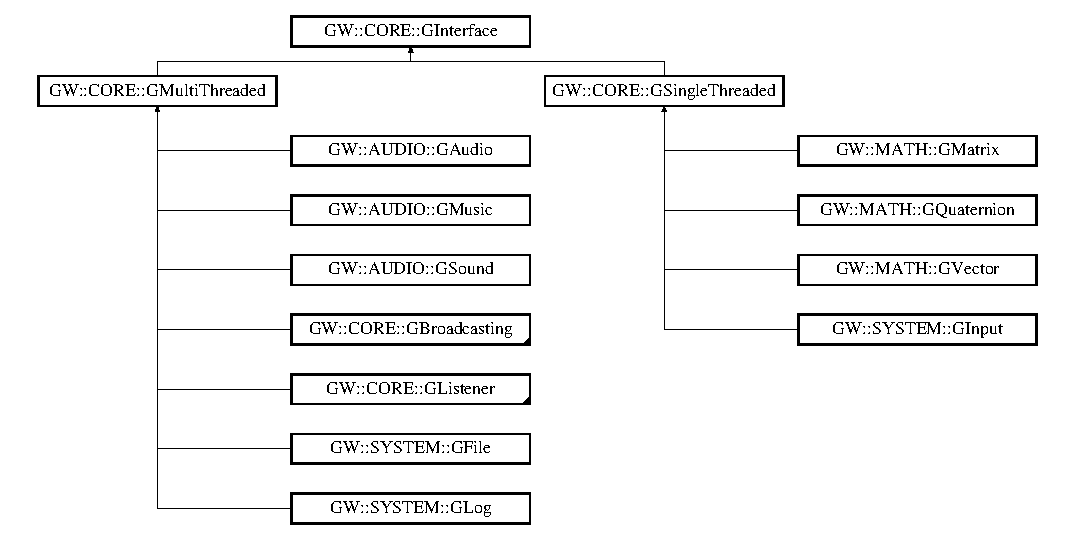
\includegraphics[height=6.810811cm]{class_g_w_1_1_c_o_r_e_1_1_g_interface}
\end{center}
\end{figure}
\subsection*{Public Member Functions}
\begin{DoxyCompactItemize}
\item 
virtual \mbox{\hyperlink{namespace_g_w_a67a839e3df7ea8a5c5686613a7a3de21}{G\+Return}} \mbox{\hyperlink{class_g_w_1_1_c_o_r_e_1_1_g_interface_aacf5834174a7024f8a3c361122ee9e76}{Get\+Count}} (unsigned int \&\+\_\+out\+Count)=0
\begin{DoxyCompactList}\small\item\em Return the total number of active references to this object. \end{DoxyCompactList}\item 
virtual \mbox{\hyperlink{namespace_g_w_a67a839e3df7ea8a5c5686613a7a3de21}{G\+Return}} \mbox{\hyperlink{class_g_w_1_1_c_o_r_e_1_1_g_interface_a2d710f20bb78e544e8309b5b75c21260}{Increment\+Count}} ()=0
\begin{DoxyCompactList}\small\item\em Increase the total number of active references to this object. \end{DoxyCompactList}\item 
virtual \mbox{\hyperlink{namespace_g_w_a67a839e3df7ea8a5c5686613a7a3de21}{G\+Return}} \mbox{\hyperlink{class_g_w_1_1_c_o_r_e_1_1_g_interface_a19a368c77ad0aa7f49b5a4f772f173ba}{Decrement\+Count}} ()=0
\begin{DoxyCompactList}\small\item\em Decrease the total number of active references to this object. \end{DoxyCompactList}\item 
virtual \mbox{\hyperlink{namespace_g_w_a67a839e3df7ea8a5c5686613a7a3de21}{G\+Return}} \mbox{\hyperlink{class_g_w_1_1_c_o_r_e_1_1_g_interface_ad6c8324970172784964f484686d4fdad}{Request\+Interface}} (const \mbox{\hyperlink{struct_g_w_1_1_g_u_u_i_i_d}{G\+U\+U\+I\+ID}} \&\+\_\+interface\+ID, void $\ast$$\ast$\+\_\+output\+Interface)=0
\begin{DoxyCompactList}\small\item\em Requests an interface that may or may not be supported by this object. \end{DoxyCompactList}\end{DoxyCompactItemize}


\subsection{Detailed Description}
Base interface all Gateware interfaces must support at a minimum. 

Core features include\+: Interface Upgrades, Reference Counting, Event Broadcasting. 

\subsection{Member Function Documentation}
\mbox{\Hypertarget{class_g_w_1_1_c_o_r_e_1_1_g_interface_a19a368c77ad0aa7f49b5a4f772f173ba}\label{class_g_w_1_1_c_o_r_e_1_1_g_interface_a19a368c77ad0aa7f49b5a4f772f173ba}} 
\index{G\+W\+::\+C\+O\+R\+E\+::\+G\+Interface@{G\+W\+::\+C\+O\+R\+E\+::\+G\+Interface}!Decrement\+Count@{Decrement\+Count}}
\index{Decrement\+Count@{Decrement\+Count}!G\+W\+::\+C\+O\+R\+E\+::\+G\+Interface@{G\+W\+::\+C\+O\+R\+E\+::\+G\+Interface}}
\subsubsection{\texorpdfstring{Decrement\+Count()}{DecrementCount()}}
{\footnotesize\ttfamily virtual \mbox{\hyperlink{namespace_g_w_a67a839e3df7ea8a5c5686613a7a3de21}{G\+Return}} G\+W\+::\+C\+O\+R\+E\+::\+G\+Interface\+::\+Decrement\+Count (\begin{DoxyParamCaption}{ }\end{DoxyParamCaption})\hspace{0.3cm}{\ttfamily [pure virtual]}}



Decrease the total number of active references to this object. 

Once the internal count reaches zero this object will be deallocated and your pointer will become invalid.


\begin{DoxyRetVals}{Return values}
{\em S\+U\+C\+C\+E\+SS} & Successfully decremented the internal reference count. \\
\hline
{\em F\+A\+I\+L\+U\+RE} & Decrementing of internal reference count would underflow the value. \\
\hline
\end{DoxyRetVals}


Implemented in \mbox{\hyperlink{class_g_w_1_1_a_u_d_i_o_1_1_g_sound_afa9587ca984fc5ad2d5cdd47c3aebbcb}{G\+W\+::\+A\+U\+D\+I\+O\+::\+G\+Sound}}, \mbox{\hyperlink{class_g_w_1_1_a_u_d_i_o_1_1_g_music_a1385376fffc42c40f5922b4722d10b5c}{G\+W\+::\+A\+U\+D\+I\+O\+::\+G\+Music}}, and \mbox{\hyperlink{class_g_w_1_1_a_u_d_i_o_1_1_g_audio_a9bdc3d4a8668b702db98dde91a0fa423}{G\+W\+::\+A\+U\+D\+I\+O\+::\+G\+Audio}}.

\mbox{\Hypertarget{class_g_w_1_1_c_o_r_e_1_1_g_interface_aacf5834174a7024f8a3c361122ee9e76}\label{class_g_w_1_1_c_o_r_e_1_1_g_interface_aacf5834174a7024f8a3c361122ee9e76}} 
\index{G\+W\+::\+C\+O\+R\+E\+::\+G\+Interface@{G\+W\+::\+C\+O\+R\+E\+::\+G\+Interface}!Get\+Count@{Get\+Count}}
\index{Get\+Count@{Get\+Count}!G\+W\+::\+C\+O\+R\+E\+::\+G\+Interface@{G\+W\+::\+C\+O\+R\+E\+::\+G\+Interface}}
\subsubsection{\texorpdfstring{Get\+Count()}{GetCount()}}
{\footnotesize\ttfamily virtual \mbox{\hyperlink{namespace_g_w_a67a839e3df7ea8a5c5686613a7a3de21}{G\+Return}} G\+W\+::\+C\+O\+R\+E\+::\+G\+Interface\+::\+Get\+Count (\begin{DoxyParamCaption}\item[{unsigned int \&}]{\+\_\+out\+Count }\end{DoxyParamCaption})\hspace{0.3cm}{\ttfamily [pure virtual]}}



Return the total number of active references to this object. 


\begin{DoxyParams}[1]{Parameters}
\mbox{\tt out}  & {\em \+\_\+out\+Count} & The total number of active references of this object.\\
\hline
\end{DoxyParams}

\begin{DoxyRetVals}{Return values}
{\em S\+U\+C\+C\+E\+SS} & Successfully ran. \\
\hline
{\em F\+A\+I\+L\+U\+RE} & Either class does not exist or the internal reference count is corrupt. \\
\hline
\end{DoxyRetVals}


Implemented in \mbox{\hyperlink{class_g_w_1_1_a_u_d_i_o_1_1_g_sound_afbac022010da2fc1a917ece2803a36a4}{G\+W\+::\+A\+U\+D\+I\+O\+::\+G\+Sound}}, \mbox{\hyperlink{class_g_w_1_1_a_u_d_i_o_1_1_g_music_ae41f54531b8325848215596fb2f821ac}{G\+W\+::\+A\+U\+D\+I\+O\+::\+G\+Music}}, and \mbox{\hyperlink{class_g_w_1_1_a_u_d_i_o_1_1_g_audio_a079dfab7b9db1536b10c9d2afa20c89c}{G\+W\+::\+A\+U\+D\+I\+O\+::\+G\+Audio}}.

\mbox{\Hypertarget{class_g_w_1_1_c_o_r_e_1_1_g_interface_a2d710f20bb78e544e8309b5b75c21260}\label{class_g_w_1_1_c_o_r_e_1_1_g_interface_a2d710f20bb78e544e8309b5b75c21260}} 
\index{G\+W\+::\+C\+O\+R\+E\+::\+G\+Interface@{G\+W\+::\+C\+O\+R\+E\+::\+G\+Interface}!Increment\+Count@{Increment\+Count}}
\index{Increment\+Count@{Increment\+Count}!G\+W\+::\+C\+O\+R\+E\+::\+G\+Interface@{G\+W\+::\+C\+O\+R\+E\+::\+G\+Interface}}
\subsubsection{\texorpdfstring{Increment\+Count()}{IncrementCount()}}
{\footnotesize\ttfamily virtual \mbox{\hyperlink{namespace_g_w_a67a839e3df7ea8a5c5686613a7a3de21}{G\+Return}} G\+W\+::\+C\+O\+R\+E\+::\+G\+Interface\+::\+Increment\+Count (\begin{DoxyParamCaption}{ }\end{DoxyParamCaption})\hspace{0.3cm}{\ttfamily [pure virtual]}}



Increase the total number of active references to this object. 

End users should only call this operation if they are familiar with reference counting behavior.


\begin{DoxyRetVals}{Return values}
{\em S\+U\+C\+C\+E\+SS} & Successfully incremented the internal reference count. \\
\hline
{\em F\+A\+I\+L\+U\+RE} & Incrementation of internal reference count would overflow the value. \\
\hline
\end{DoxyRetVals}


Implemented in \mbox{\hyperlink{class_g_w_1_1_a_u_d_i_o_1_1_g_sound_a33149257f0958b4db57f5508492410ad}{G\+W\+::\+A\+U\+D\+I\+O\+::\+G\+Sound}}, \mbox{\hyperlink{class_g_w_1_1_a_u_d_i_o_1_1_g_music_a22d7a170b4d307e5398ebb92f950431f}{G\+W\+::\+A\+U\+D\+I\+O\+::\+G\+Music}}, and \mbox{\hyperlink{class_g_w_1_1_a_u_d_i_o_1_1_g_audio_aba5697a3a308026ecaa12737d6fe6705}{G\+W\+::\+A\+U\+D\+I\+O\+::\+G\+Audio}}.

\mbox{\Hypertarget{class_g_w_1_1_c_o_r_e_1_1_g_interface_ad6c8324970172784964f484686d4fdad}\label{class_g_w_1_1_c_o_r_e_1_1_g_interface_ad6c8324970172784964f484686d4fdad}} 
\index{G\+W\+::\+C\+O\+R\+E\+::\+G\+Interface@{G\+W\+::\+C\+O\+R\+E\+::\+G\+Interface}!Request\+Interface@{Request\+Interface}}
\index{Request\+Interface@{Request\+Interface}!G\+W\+::\+C\+O\+R\+E\+::\+G\+Interface@{G\+W\+::\+C\+O\+R\+E\+::\+G\+Interface}}
\subsubsection{\texorpdfstring{Request\+Interface()}{RequestInterface()}}
{\footnotesize\ttfamily virtual \mbox{\hyperlink{namespace_g_w_a67a839e3df7ea8a5c5686613a7a3de21}{G\+Return}} G\+W\+::\+C\+O\+R\+E\+::\+G\+Interface\+::\+Request\+Interface (\begin{DoxyParamCaption}\item[{const \mbox{\hyperlink{struct_g_w_1_1_g_u_u_i_i_d}{G\+U\+U\+I\+ID}} \&}]{\+\_\+interface\+ID,  }\item[{void $\ast$$\ast$}]{\+\_\+output\+Interface }\end{DoxyParamCaption})\hspace{0.3cm}{\ttfamily [pure virtual]}}



Requests an interface that may or may not be supported by this object. 

Can be used by the end-\/user to query for a new interface using the unique ID of the interface they want and implement an interface update.


\begin{DoxyParams}[1]{Parameters}
\mbox{\tt in}  & {\em \+\_\+interface\+ID} & The \mbox{\hyperlink{struct_g_w_1_1_g_u_u_i_i_d}{G\+U\+U\+I\+ID}} of the interface you are requesting. \\
\hline
\mbox{\tt out}  & {\em \+\_\+output\+Interface} & Where the interface will be stored if function is successful.\\
\hline
\end{DoxyParams}

\begin{DoxyRetVals}{Return values}
{\em S\+U\+C\+C\+E\+SS} & The interface is supported and function succeded. \\
\hline
{\em I\+N\+T\+E\+R\+F\+A\+C\+E\+\_\+\+U\+N\+S\+U\+P\+P\+O\+R\+T\+ED} & The requested interface is not supported. \\
\hline
\end{DoxyRetVals}


Implemented in \mbox{\hyperlink{class_g_w_1_1_a_u_d_i_o_1_1_g_sound_ac3c8f8dd06b71f86356a3e316fb3b4dc}{G\+W\+::\+A\+U\+D\+I\+O\+::\+G\+Sound}}, \mbox{\hyperlink{class_g_w_1_1_a_u_d_i_o_1_1_g_music_a45b07d7915cfe61ab27338c42b78dcfb}{G\+W\+::\+A\+U\+D\+I\+O\+::\+G\+Music}}, and \mbox{\hyperlink{class_g_w_1_1_a_u_d_i_o_1_1_g_audio_a29561ad9852a36dd14746adbaac21c80}{G\+W\+::\+A\+U\+D\+I\+O\+::\+G\+Audio}}.



The documentation for this class was generated from the following file\+:\begin{DoxyCompactItemize}
\item 
C\+:/\+Users/\+Devin Wright/\+Documents/\+Gate\+Ware\+Repo/gateware.\+git.\+0/\+Interface/\+G\+\_\+\+Core/G\+Interface.\+h\end{DoxyCompactItemize}

\hypertarget{class_g_w_1_1_c_o_r_e_1_1_g_listener}{}\section{GW\+:\+:C\+O\+RE\+:\+:G\+Listener Class Reference}
\label{class_g_w_1_1_c_o_r_e_1_1_g_listener}\index{G\+W\+::\+C\+O\+R\+E\+::\+G\+Listener@{G\+W\+::\+C\+O\+R\+E\+::\+G\+Listener}}


A \mbox{\hyperlink{class_g_w_1_1_c_o_r_e_1_1_g_listener}{G\+Listener}} Interface may be registered with a G\+Broadcaster interface to receive event notifications.  




{\ttfamily \#include $<$G\+Listener.\+h$>$}

Inheritance diagram for GW\+:\+:C\+O\+RE\+:\+:G\+Listener\+:\begin{figure}[H]
\begin{center}
\leavevmode
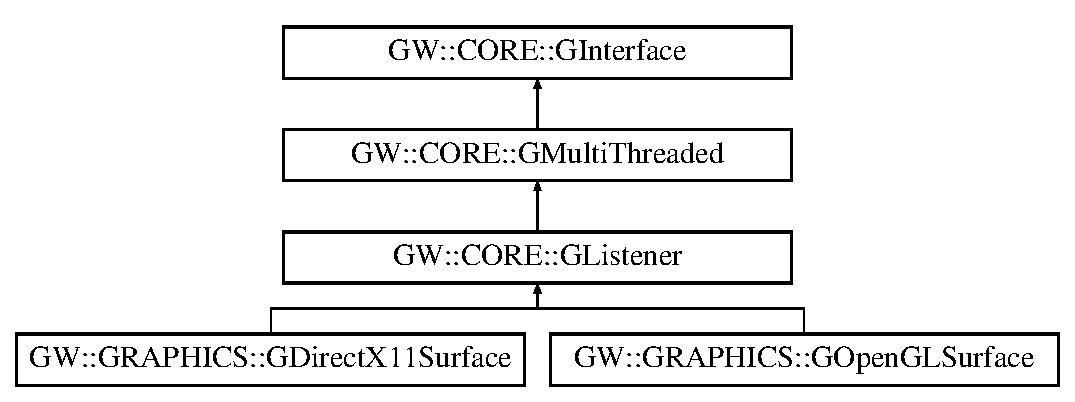
\includegraphics[height=4.000000cm]{class_g_w_1_1_c_o_r_e_1_1_g_listener}
\end{center}
\end{figure}
\subsection*{Public Member Functions}
\begin{DoxyCompactItemize}
\item 
virtual \mbox{\hyperlink{namespace_g_w_a67a839e3df7ea8a5c5686613a7a3de21}{G\+Return}} \mbox{\hyperlink{class_g_w_1_1_c_o_r_e_1_1_g_listener_a5c1d1fac213b7a1cc15d384aa0c33105}{On\+Event}} (const \mbox{\hyperlink{struct_g_w_1_1_g_u_u_i_i_d}{G\+U\+U\+I\+ID}} \&\+\_\+sender\+Interface, unsigned int \+\_\+event\+ID, void $\ast$\+\_\+event\+Data, unsigned int \+\_\+data\+Size)=0
\begin{DoxyCompactList}\small\item\em This operation is called whenever a G\+Broadcaster a listener is registered to generates an event. \end{DoxyCompactList}\end{DoxyCompactItemize}


\subsection{Detailed Description}
A \mbox{\hyperlink{class_g_w_1_1_c_o_r_e_1_1_g_listener}{G\+Listener}} Interface may be registered with a G\+Broadcaster interface to receive event notifications. 

\mbox{\hyperlink{class_g_w_1_1_c_o_r_e_1_1_g_listener}{G\+Listener}} is directly inherited from \mbox{\hyperlink{class_g_w_1_1_c_o_r_e_1_1_g_multi_threaded}{G\+Multi\+Threaded}}, therefore its implementation must be thread safe. 

\subsection{Member Function Documentation}
\mbox{\Hypertarget{class_g_w_1_1_c_o_r_e_1_1_g_listener_a5c1d1fac213b7a1cc15d384aa0c33105}\label{class_g_w_1_1_c_o_r_e_1_1_g_listener_a5c1d1fac213b7a1cc15d384aa0c33105}} 
\index{G\+W\+::\+C\+O\+R\+E\+::\+G\+Listener@{G\+W\+::\+C\+O\+R\+E\+::\+G\+Listener}!On\+Event@{On\+Event}}
\index{On\+Event@{On\+Event}!G\+W\+::\+C\+O\+R\+E\+::\+G\+Listener@{G\+W\+::\+C\+O\+R\+E\+::\+G\+Listener}}
\subsubsection{\texorpdfstring{On\+Event()}{OnEvent()}}
{\footnotesize\ttfamily virtual \mbox{\hyperlink{namespace_g_w_a67a839e3df7ea8a5c5686613a7a3de21}{G\+Return}} G\+W\+::\+C\+O\+R\+E\+::\+G\+Listener\+::\+On\+Event (\begin{DoxyParamCaption}\item[{const \mbox{\hyperlink{struct_g_w_1_1_g_u_u_i_i_d}{G\+U\+U\+I\+ID}} \&}]{\+\_\+sender\+Interface,  }\item[{unsigned int}]{\+\_\+event\+ID,  }\item[{void $\ast$}]{\+\_\+event\+Data,  }\item[{unsigned int}]{\+\_\+data\+Size }\end{DoxyParamCaption})\hspace{0.3cm}{\ttfamily [pure virtual]}}



This operation is called whenever a G\+Broadcaster a listener is registered to generates an event. 


\begin{DoxyParams}[1]{Parameters}
\mbox{\tt in}  & {\em \+\_\+sender\+Interface} & The interface of the sender object. \\
\hline
\mbox{\tt in}  & {\em \+\_\+event\+ID} & The ID of the event sent. \\
\hline
\mbox{\tt in}  & {\em \+\_\+event\+Data} & The data of the event. \\
\hline
\mbox{\tt in}  & {\em \+\_\+data\+Size} & The size of \+\_\+event\+Data in bytes. \\
\hline
\end{DoxyParams}


The documentation for this class was generated from the following file\+:\begin{DoxyCompactItemize}
\item 
G\+\_\+\+Core/G\+Listener.\+h\end{DoxyCompactItemize}

\hypertarget{class_g_w_1_1_c_o_r_e_1_1_g_log}{}\section{GW\+:\+:C\+O\+RE\+:\+:G\+Log Class Reference}
\label{class_g_w_1_1_c_o_r_e_1_1_g_log}\index{G\+W\+::\+C\+O\+R\+E\+::\+G\+Log@{G\+W\+::\+C\+O\+R\+E\+::\+G\+Log}}


Cross platform threadsafe logger.  




{\ttfamily \#include $<$G\+Log.\+h$>$}



Inherits \hyperlink{class_g_w_1_1_c_o_r_e_1_1_g_multi_threaded}{G\+W\+::\+C\+O\+R\+E\+::\+G\+Multi\+Threaded}.

\subsection*{Public Member Functions}
\begin{DoxyCompactItemize}
\item 
virtual \hyperlink{namespace_g_w_a69b1aaebac1cac8049825f035884c95b}{G\+R\+E\+T\+U\+RN} \hyperlink{class_g_w_1_1_c_o_r_e_1_1_g_log_a9b9ec52b1b35eb2fd9a63ec7312fd31a}{Log} (const char $\ast$const \+\_\+log)=0
\begin{DoxyCompactList}\small\item\em Logs a null terminated string. \end{DoxyCompactList}\item 
virtual \hyperlink{namespace_g_w_a69b1aaebac1cac8049825f035884c95b}{G\+R\+E\+T\+U\+RN} \hyperlink{class_g_w_1_1_c_o_r_e_1_1_g_log_ab7dbe43179c1de11c9ddac9d6cba01cf}{Log\+Catergorized} (const char $\ast$const \+\_\+category, const char $\ast$const \+\_\+log)=0
\begin{DoxyCompactList}\small\item\em Logs a null terminated string with a category. \end{DoxyCompactList}\item 
virtual void \hyperlink{class_g_w_1_1_c_o_r_e_1_1_g_log_ac14e65291dba9480deadd772a8f0e307}{Enable\+Verbose\+Logging} (bool \+\_\+value)=0
\begin{DoxyCompactList}\small\item\em Turns verbose logging on or off. \end{DoxyCompactList}\item 
virtual void \hyperlink{class_g_w_1_1_c_o_r_e_1_1_g_log_a9a486a646a0a02bb5724100c1849fcec}{Enable\+Console\+Logging} (bool \+\_\+value)=0
\begin{DoxyCompactList}\small\item\em Turns console logging on or off. \end{DoxyCompactList}\item 
virtual \hyperlink{namespace_g_w_a69b1aaebac1cac8049825f035884c95b}{G\+R\+E\+T\+U\+RN} \hyperlink{class_g_w_1_1_c_o_r_e_1_1_g_log_a1e0bb42d95ddd42fa019d5cd6050ff97}{Flush} ()=0
\begin{DoxyCompactList}\small\item\em Forces a log dump to file. \end{DoxyCompactList}\item 
virtual \hyperlink{namespace_g_w_a69b1aaebac1cac8049825f035884c95b}{G\+R\+E\+T\+U\+RN} \hyperlink{class_g_w_1_1_c_o_r_e_1_1_g_interface_a80f212dcdf60202cf9da49405863d1d5}{Get\+Count} (unsigned int \&\+\_\+out\+Count)=0
\begin{DoxyCompactList}\small\item\em Return the total number of active refrences to this object. \end{DoxyCompactList}\item 
virtual \hyperlink{namespace_g_w_a69b1aaebac1cac8049825f035884c95b}{G\+R\+E\+T\+U\+RN} \hyperlink{class_g_w_1_1_c_o_r_e_1_1_g_interface_a3e04e58eef4f3e3f56ff7fb751194c37}{Increment\+Count} ()=0
\begin{DoxyCompactList}\small\item\em Increase the total number of active refrences to this object. \end{DoxyCompactList}\item 
virtual \hyperlink{namespace_g_w_a69b1aaebac1cac8049825f035884c95b}{G\+R\+E\+T\+U\+RN} \hyperlink{class_g_w_1_1_c_o_r_e_1_1_g_interface_af6924e12b14f217b518fc91c63d9703d}{Decrement\+Count} ()=0
\begin{DoxyCompactList}\small\item\em Decrease the total number of active refrences to this object. \end{DoxyCompactList}\item 
virtual \hyperlink{namespace_g_w_a69b1aaebac1cac8049825f035884c95b}{G\+R\+E\+T\+U\+RN} \hyperlink{class_g_w_1_1_c_o_r_e_1_1_g_interface_ab1414aa07bca310a824ee01a91657ad0}{Request\+Interface} (const \hyperlink{struct_g_w_1_1_g_u_u_i_i_d}{G\+U\+U\+I\+ID} \&\+\_\+interface\+ID, void $\ast$$\ast$\+\_\+output\+Interface)=0
\begin{DoxyCompactList}\small\item\em Requests an interface that may or may not be supported by this object. \end{DoxyCompactList}\end{DoxyCompactItemize}


\subsection{Member Function Documentation}
\hypertarget{class_g_w_1_1_c_o_r_e_1_1_g_interface_af6924e12b14f217b518fc91c63d9703d}{}\label{class_g_w_1_1_c_o_r_e_1_1_g_interface_af6924e12b14f217b518fc91c63d9703d} 
\index{G\+W\+::\+C\+O\+R\+E\+::\+G\+Log@{G\+W\+::\+C\+O\+R\+E\+::\+G\+Log}!Decrement\+Count@{Decrement\+Count}}
\index{Decrement\+Count@{Decrement\+Count}!G\+W\+::\+C\+O\+R\+E\+::\+G\+Log@{G\+W\+::\+C\+O\+R\+E\+::\+G\+Log}}
\subsubsection{\texorpdfstring{Decrement\+Count()}{DecrementCount()}}
{\footnotesize\ttfamily virtual \hyperlink{namespace_g_w_a69b1aaebac1cac8049825f035884c95b}{G\+R\+E\+T\+U\+RN} G\+W\+::\+C\+O\+R\+E\+::\+G\+Interface\+::\+Decrement\+Count (\begin{DoxyParamCaption}{ }\end{DoxyParamCaption})\hspace{0.3cm}{\ttfamily [pure virtual]}, {\ttfamily [inherited]}}

Once the internal count reaches zero this object will be deallocated and your pointer will become invalid.


\begin{DoxyRetVals}{Return values}
{\em S\+U\+C\+C\+E\+SS} & Successfully decremented the internal reference count. \\
\hline
{\em F\+A\+I\+L\+U\+RE} & Decrementing of internal reference count would underflow the value. \\
\hline
\end{DoxyRetVals}
\hypertarget{class_g_w_1_1_c_o_r_e_1_1_g_log_a9a486a646a0a02bb5724100c1849fcec}{}\label{class_g_w_1_1_c_o_r_e_1_1_g_log_a9a486a646a0a02bb5724100c1849fcec} 
\index{G\+W\+::\+C\+O\+R\+E\+::\+G\+Log@{G\+W\+::\+C\+O\+R\+E\+::\+G\+Log}!Enable\+Console\+Logging@{Enable\+Console\+Logging}}
\index{Enable\+Console\+Logging@{Enable\+Console\+Logging}!G\+W\+::\+C\+O\+R\+E\+::\+G\+Log@{G\+W\+::\+C\+O\+R\+E\+::\+G\+Log}}
\subsubsection{\texorpdfstring{Enable\+Console\+Logging()}{EnableConsoleLogging()}}
{\footnotesize\ttfamily virtual void G\+W\+::\+C\+O\+R\+E\+::\+G\+Log\+::\+Enable\+Console\+Logging (\begin{DoxyParamCaption}\item[{bool}]{\+\_\+value }\end{DoxyParamCaption})\hspace{0.3cm}{\ttfamily [pure virtual]}}

Use this function to prevent the additional console logging.


\begin{DoxyParams}[1]{Parameters}
\mbox{\tt in}  & {\em \+\_\+value} & true to turn on or false to turn off. \\
\hline
\end{DoxyParams}
\hypertarget{class_g_w_1_1_c_o_r_e_1_1_g_log_ac14e65291dba9480deadd772a8f0e307}{}\label{class_g_w_1_1_c_o_r_e_1_1_g_log_ac14e65291dba9480deadd772a8f0e307} 
\index{G\+W\+::\+C\+O\+R\+E\+::\+G\+Log@{G\+W\+::\+C\+O\+R\+E\+::\+G\+Log}!Enable\+Verbose\+Logging@{Enable\+Verbose\+Logging}}
\index{Enable\+Verbose\+Logging@{Enable\+Verbose\+Logging}!G\+W\+::\+C\+O\+R\+E\+::\+G\+Log@{G\+W\+::\+C\+O\+R\+E\+::\+G\+Log}}
\subsubsection{\texorpdfstring{Enable\+Verbose\+Logging()}{EnableVerboseLogging()}}
{\footnotesize\ttfamily virtual void G\+W\+::\+C\+O\+R\+E\+::\+G\+Log\+::\+Enable\+Verbose\+Logging (\begin{DoxyParamCaption}\item[{bool}]{\+\_\+value }\end{DoxyParamCaption})\hspace{0.3cm}{\ttfamily [pure virtual]}}

Use this function to prevent the addition of date, time, and thread\+ID to your logs.


\begin{DoxyParams}[1]{Parameters}
\mbox{\tt in}  & {\em \+\_\+value} & true to turn on or false to turn off. \\
\hline
\end{DoxyParams}
\hypertarget{class_g_w_1_1_c_o_r_e_1_1_g_log_a1e0bb42d95ddd42fa019d5cd6050ff97}{}\label{class_g_w_1_1_c_o_r_e_1_1_g_log_a1e0bb42d95ddd42fa019d5cd6050ff97} 
\index{G\+W\+::\+C\+O\+R\+E\+::\+G\+Log@{G\+W\+::\+C\+O\+R\+E\+::\+G\+Log}!Flush@{Flush}}
\index{Flush@{Flush}!G\+W\+::\+C\+O\+R\+E\+::\+G\+Log@{G\+W\+::\+C\+O\+R\+E\+::\+G\+Log}}
\subsubsection{\texorpdfstring{Flush()}{Flush()}}
{\footnotesize\ttfamily virtual \hyperlink{namespace_g_w_a69b1aaebac1cac8049825f035884c95b}{G\+R\+E\+T\+U\+RN} G\+W\+::\+C\+O\+R\+E\+::\+G\+Log\+::\+Flush (\begin{DoxyParamCaption}{ }\end{DoxyParamCaption})\hspace{0.3cm}{\ttfamily [pure virtual]}}

This will force a log dump to the file and clear the log queue.


\begin{DoxyRetVals}{Return values}
{\em S\+U\+C\+C\+E\+SS} & Successfully dumped the logs \\
\hline
{\em F\+A\+I\+L\+U\+RE} & Most likely a file corruption or a file is not open. \\
\hline
\end{DoxyRetVals}
\hypertarget{class_g_w_1_1_c_o_r_e_1_1_g_interface_a80f212dcdf60202cf9da49405863d1d5}{}\label{class_g_w_1_1_c_o_r_e_1_1_g_interface_a80f212dcdf60202cf9da49405863d1d5} 
\index{G\+W\+::\+C\+O\+R\+E\+::\+G\+Log@{G\+W\+::\+C\+O\+R\+E\+::\+G\+Log}!Get\+Count@{Get\+Count}}
\index{Get\+Count@{Get\+Count}!G\+W\+::\+C\+O\+R\+E\+::\+G\+Log@{G\+W\+::\+C\+O\+R\+E\+::\+G\+Log}}
\subsubsection{\texorpdfstring{Get\+Count()}{GetCount()}}
{\footnotesize\ttfamily virtual \hyperlink{namespace_g_w_a69b1aaebac1cac8049825f035884c95b}{G\+R\+E\+T\+U\+RN} G\+W\+::\+C\+O\+R\+E\+::\+G\+Interface\+::\+Get\+Count (\begin{DoxyParamCaption}\item[{unsigned int \&}]{\+\_\+out\+Count }\end{DoxyParamCaption})\hspace{0.3cm}{\ttfamily [pure virtual]}, {\ttfamily [inherited]}}


\begin{DoxyParams}[1]{Parameters}
\mbox{\tt out}  & {\em \+\_\+out\+Count} & The total number of active references of this object.\\
\hline
\end{DoxyParams}

\begin{DoxyRetVals}{Return values}
{\em S\+U\+C\+C\+E\+SS} & Successfully ran \\
\hline
{\em F\+A\+I\+L\+U\+RE} & Either class does not exist or the internal reference count is corupt. \\
\hline
\end{DoxyRetVals}
\hypertarget{class_g_w_1_1_c_o_r_e_1_1_g_interface_a3e04e58eef4f3e3f56ff7fb751194c37}{}\label{class_g_w_1_1_c_o_r_e_1_1_g_interface_a3e04e58eef4f3e3f56ff7fb751194c37} 
\index{G\+W\+::\+C\+O\+R\+E\+::\+G\+Log@{G\+W\+::\+C\+O\+R\+E\+::\+G\+Log}!Increment\+Count@{Increment\+Count}}
\index{Increment\+Count@{Increment\+Count}!G\+W\+::\+C\+O\+R\+E\+::\+G\+Log@{G\+W\+::\+C\+O\+R\+E\+::\+G\+Log}}
\subsubsection{\texorpdfstring{Increment\+Count()}{IncrementCount()}}
{\footnotesize\ttfamily virtual \hyperlink{namespace_g_w_a69b1aaebac1cac8049825f035884c95b}{G\+R\+E\+T\+U\+RN} G\+W\+::\+C\+O\+R\+E\+::\+G\+Interface\+::\+Increment\+Count (\begin{DoxyParamCaption}{ }\end{DoxyParamCaption})\hspace{0.3cm}{\ttfamily [pure virtual]}, {\ttfamily [inherited]}}

End users should only call this operation if they are familiar with reference counting behavior.


\begin{DoxyRetVals}{Return values}
{\em S\+U\+C\+C\+E\+SS} & Successfully incremented the internal reference count. \\
\hline
{\em F\+A\+I\+L\+U\+RE} & Incrementation of internal reference count would overflow the value. \\
\hline
\end{DoxyRetVals}
\hypertarget{class_g_w_1_1_c_o_r_e_1_1_g_log_a9b9ec52b1b35eb2fd9a63ec7312fd31a}{}\label{class_g_w_1_1_c_o_r_e_1_1_g_log_a9b9ec52b1b35eb2fd9a63ec7312fd31a} 
\index{G\+W\+::\+C\+O\+R\+E\+::\+G\+Log@{G\+W\+::\+C\+O\+R\+E\+::\+G\+Log}!Log@{Log}}
\index{Log@{Log}!G\+W\+::\+C\+O\+R\+E\+::\+G\+Log@{G\+W\+::\+C\+O\+R\+E\+::\+G\+Log}}
\subsubsection{\texorpdfstring{Log()}{Log()}}
{\footnotesize\ttfamily virtual \hyperlink{namespace_g_w_a69b1aaebac1cac8049825f035884c95b}{G\+R\+E\+T\+U\+RN} G\+W\+::\+C\+O\+R\+E\+::\+G\+Log\+::\+Log (\begin{DoxyParamCaption}\item[{const char $\ast$const}]{\+\_\+log }\end{DoxyParamCaption})\hspace{0.3cm}{\ttfamily [pure virtual]}}

Date, Time, and thread ID will be appended to the front of the message unless specified otherwise (See Enable\+Verbose\+Logging). A new line character will be appended to the end of the string so your log messages do not require a new line.


\begin{DoxyParams}[1]{Parameters}
\mbox{\tt in}  & {\em \+\_\+log} & The message to log out.\\
\hline
\end{DoxyParams}

\begin{DoxyRetVals}{Return values}
{\em S\+U\+C\+C\+E\+SS} & Successfully queued the message to the log. \\
\hline
{\em F\+A\+I\+L\+U\+RE} & The queue has reached maximun size (call flush). \\
\hline
{\em I\+N\+V\+A\+L\+I\+D\+\_\+\+A\+R\+G\+U\+M\+E\+NT} & A nullptr was passed in. \\
\hline
\end{DoxyRetVals}
\hypertarget{class_g_w_1_1_c_o_r_e_1_1_g_log_ab7dbe43179c1de11c9ddac9d6cba01cf}{}\label{class_g_w_1_1_c_o_r_e_1_1_g_log_ab7dbe43179c1de11c9ddac9d6cba01cf} 
\index{G\+W\+::\+C\+O\+R\+E\+::\+G\+Log@{G\+W\+::\+C\+O\+R\+E\+::\+G\+Log}!Log\+Catergorized@{Log\+Catergorized}}
\index{Log\+Catergorized@{Log\+Catergorized}!G\+W\+::\+C\+O\+R\+E\+::\+G\+Log@{G\+W\+::\+C\+O\+R\+E\+::\+G\+Log}}
\subsubsection{\texorpdfstring{Log\+Catergorized()}{LogCatergorized()}}
{\footnotesize\ttfamily virtual \hyperlink{namespace_g_w_a69b1aaebac1cac8049825f035884c95b}{G\+R\+E\+T\+U\+RN} G\+W\+::\+C\+O\+R\+E\+::\+G\+Log\+::\+Log\+Catergorized (\begin{DoxyParamCaption}\item[{const char $\ast$const}]{\+\_\+category,  }\item[{const char $\ast$const}]{\+\_\+log }\end{DoxyParamCaption})\hspace{0.3cm}{\ttfamily [pure virtual]}}

Date, Time, and thread ID will be appended to the front of the message unless specified otherwise (See Enable\+Verbose\+Logging). A new line character will be appended to the end of the string so your log messages do not require a new line.


\begin{DoxyParams}[1]{Parameters}
\mbox{\tt in}  & {\em \+\_\+category} & The category the log belongs in. ie. E\+R\+R\+OR, W\+A\+R\+N\+I\+NG, I\+N\+FO, etc. \\
\hline
\mbox{\tt in}  & {\em \+\_\+log} & The message to log out.\\
\hline
\end{DoxyParams}

\begin{DoxyRetVals}{Return values}
{\em S\+U\+C\+C\+E\+SS} & Successfully queued the message to the log. \\
\hline
{\em F\+A\+I\+L\+U\+RE} & The queue has reached maximun size (call flush). \\
\hline
{\em I\+N\+V\+A\+L\+I\+D\+\_\+\+A\+R\+G\+U\+M\+E\+NT} & Either \+\_\+category or \+\_\+log are nullptr. \\
\hline
\end{DoxyRetVals}
\hypertarget{class_g_w_1_1_c_o_r_e_1_1_g_interface_ab1414aa07bca310a824ee01a91657ad0}{}\label{class_g_w_1_1_c_o_r_e_1_1_g_interface_ab1414aa07bca310a824ee01a91657ad0} 
\index{G\+W\+::\+C\+O\+R\+E\+::\+G\+Log@{G\+W\+::\+C\+O\+R\+E\+::\+G\+Log}!Request\+Interface@{Request\+Interface}}
\index{Request\+Interface@{Request\+Interface}!G\+W\+::\+C\+O\+R\+E\+::\+G\+Log@{G\+W\+::\+C\+O\+R\+E\+::\+G\+Log}}
\subsubsection{\texorpdfstring{Request\+Interface()}{RequestInterface()}}
{\footnotesize\ttfamily virtual \hyperlink{namespace_g_w_a69b1aaebac1cac8049825f035884c95b}{G\+R\+E\+T\+U\+RN} G\+W\+::\+C\+O\+R\+E\+::\+G\+Interface\+::\+Request\+Interface (\begin{DoxyParamCaption}\item[{const \hyperlink{struct_g_w_1_1_g_u_u_i_i_d}{G\+U\+U\+I\+ID} \&}]{\+\_\+interface\+ID,  }\item[{void $\ast$$\ast$}]{\+\_\+output\+Interface }\end{DoxyParamCaption})\hspace{0.3cm}{\ttfamily [pure virtual]}, {\ttfamily [inherited]}}

Similiar to DirectX query\+Interface function.


\begin{DoxyParams}[1]{Parameters}
\mbox{\tt in}  & {\em \+\_\+interface\+ID} & The \hyperlink{struct_g_w_1_1_g_u_u_i_i_d}{G\+U\+U\+I\+ID} of the interface you are requesting. \\
\hline
\mbox{\tt out}  & {\em \+\_\+output\+Interface} & Where the interface will be stored if function is successful.\\
\hline
\end{DoxyParams}

\begin{DoxyRetVals}{Return values}
{\em S\+U\+C\+C\+E\+SS} & The interface is support and function succeded. \\
\hline
{\em I\+N\+T\+E\+R\+F\+A\+C\+E\+\_\+\+U\+N\+S\+U\+P\+P\+O\+R\+T\+ED} & The requested interface is not supported. \\
\hline
\end{DoxyRetVals}


The documentation for this class was generated from the following file\+:\begin{DoxyCompactItemize}
\item 
G\+Log.\+h\end{DoxyCompactItemize}

\hypertarget{class_g_w_1_1_c_o_r_e_1_1_g_multi_threaded}{}\section{GW\+:\+:C\+O\+RE\+:\+:G\+Multi\+Threaded Class Reference}
\label{class_g_w_1_1_c_o_r_e_1_1_g_multi_threaded}\index{G\+W\+::\+C\+O\+R\+E\+::\+G\+Multi\+Threaded@{G\+W\+::\+C\+O\+R\+E\+::\+G\+Multi\+Threaded}}


This interface is only used to label and query interfaces which promise to 100\% internally support thread saftey.  




{\ttfamily \#include $<$G\+Multi\+Threaded.\+h$>$}



Inherits \hyperlink{class_g_w_1_1_c_o_r_e_1_1_g_interface}{G\+W\+::\+C\+O\+R\+E\+::\+G\+Interface}.



Inherited by \hyperlink{class_g_w_1_1_c_o_r_e_1_1_g_broadcasting}{G\+W\+::\+C\+O\+R\+E\+::\+G\+Broadcasting}, \hyperlink{class_g_w_1_1_c_o_r_e_1_1_g_file}{G\+W\+::\+C\+O\+R\+E\+::\+G\+File}, \hyperlink{class_g_w_1_1_c_o_r_e_1_1_g_listener}{G\+W\+::\+C\+O\+R\+E\+::\+G\+Listener}, and \hyperlink{class_g_w_1_1_c_o_r_e_1_1_g_log}{G\+W\+::\+C\+O\+R\+E\+::\+G\+Log}.

\subsection*{Public Member Functions}
\begin{DoxyCompactItemize}
\item 
virtual \hyperlink{namespace_g_w_a69b1aaebac1cac8049825f035884c95b}{G\+R\+E\+T\+U\+RN} \hyperlink{class_g_w_1_1_c_o_r_e_1_1_g_interface_a80f212dcdf60202cf9da49405863d1d5}{Get\+Count} (unsigned int \&\+\_\+out\+Count)=0
\begin{DoxyCompactList}\small\item\em Return the total number of active refrences to this object. \end{DoxyCompactList}\item 
virtual \hyperlink{namespace_g_w_a69b1aaebac1cac8049825f035884c95b}{G\+R\+E\+T\+U\+RN} \hyperlink{class_g_w_1_1_c_o_r_e_1_1_g_interface_a3e04e58eef4f3e3f56ff7fb751194c37}{Increment\+Count} ()=0
\begin{DoxyCompactList}\small\item\em Increase the total number of active refrences to this object. \end{DoxyCompactList}\item 
virtual \hyperlink{namespace_g_w_a69b1aaebac1cac8049825f035884c95b}{G\+R\+E\+T\+U\+RN} \hyperlink{class_g_w_1_1_c_o_r_e_1_1_g_interface_af6924e12b14f217b518fc91c63d9703d}{Decrement\+Count} ()=0
\begin{DoxyCompactList}\small\item\em Decrease the total number of active refrences to this object. \end{DoxyCompactList}\item 
virtual \hyperlink{namespace_g_w_a69b1aaebac1cac8049825f035884c95b}{G\+R\+E\+T\+U\+RN} \hyperlink{class_g_w_1_1_c_o_r_e_1_1_g_interface_ab1414aa07bca310a824ee01a91657ad0}{Request\+Interface} (const \hyperlink{struct_g_w_1_1_g_u_u_i_i_d}{G\+U\+U\+I\+ID} \&\+\_\+interface\+ID, void $\ast$$\ast$\+\_\+output\+Interface)=0
\begin{DoxyCompactList}\small\item\em Requests an interface that may or may not be supported by this object. \end{DoxyCompactList}\end{DoxyCompactItemize}


\subsection{Member Function Documentation}
\hypertarget{class_g_w_1_1_c_o_r_e_1_1_g_interface_af6924e12b14f217b518fc91c63d9703d}{}\label{class_g_w_1_1_c_o_r_e_1_1_g_interface_af6924e12b14f217b518fc91c63d9703d} 
\index{G\+W\+::\+C\+O\+R\+E\+::\+G\+Multi\+Threaded@{G\+W\+::\+C\+O\+R\+E\+::\+G\+Multi\+Threaded}!Decrement\+Count@{Decrement\+Count}}
\index{Decrement\+Count@{Decrement\+Count}!G\+W\+::\+C\+O\+R\+E\+::\+G\+Multi\+Threaded@{G\+W\+::\+C\+O\+R\+E\+::\+G\+Multi\+Threaded}}
\subsubsection{\texorpdfstring{Decrement\+Count()}{DecrementCount()}}
{\footnotesize\ttfamily virtual \hyperlink{namespace_g_w_a69b1aaebac1cac8049825f035884c95b}{G\+R\+E\+T\+U\+RN} G\+W\+::\+C\+O\+R\+E\+::\+G\+Interface\+::\+Decrement\+Count (\begin{DoxyParamCaption}{ }\end{DoxyParamCaption})\hspace{0.3cm}{\ttfamily [pure virtual]}, {\ttfamily [inherited]}}

Once the internal count reaches zero this object will be deallocated and your pointer will become invalid.


\begin{DoxyRetVals}{Return values}
{\em S\+U\+C\+C\+E\+SS} & Successfully decremented the internal reference count. \\
\hline
{\em F\+A\+I\+L\+U\+RE} & Decrementing of internal reference count would underflow the value. \\
\hline
\end{DoxyRetVals}
\hypertarget{class_g_w_1_1_c_o_r_e_1_1_g_interface_a80f212dcdf60202cf9da49405863d1d5}{}\label{class_g_w_1_1_c_o_r_e_1_1_g_interface_a80f212dcdf60202cf9da49405863d1d5} 
\index{G\+W\+::\+C\+O\+R\+E\+::\+G\+Multi\+Threaded@{G\+W\+::\+C\+O\+R\+E\+::\+G\+Multi\+Threaded}!Get\+Count@{Get\+Count}}
\index{Get\+Count@{Get\+Count}!G\+W\+::\+C\+O\+R\+E\+::\+G\+Multi\+Threaded@{G\+W\+::\+C\+O\+R\+E\+::\+G\+Multi\+Threaded}}
\subsubsection{\texorpdfstring{Get\+Count()}{GetCount()}}
{\footnotesize\ttfamily virtual \hyperlink{namespace_g_w_a69b1aaebac1cac8049825f035884c95b}{G\+R\+E\+T\+U\+RN} G\+W\+::\+C\+O\+R\+E\+::\+G\+Interface\+::\+Get\+Count (\begin{DoxyParamCaption}\item[{unsigned int \&}]{\+\_\+out\+Count }\end{DoxyParamCaption})\hspace{0.3cm}{\ttfamily [pure virtual]}, {\ttfamily [inherited]}}


\begin{DoxyParams}[1]{Parameters}
\mbox{\tt out}  & {\em \+\_\+out\+Count} & The total number of active references of this object.\\
\hline
\end{DoxyParams}

\begin{DoxyRetVals}{Return values}
{\em S\+U\+C\+C\+E\+SS} & Successfully ran \\
\hline
{\em F\+A\+I\+L\+U\+RE} & Either class does not exist or the internal reference count is corupt. \\
\hline
\end{DoxyRetVals}
\hypertarget{class_g_w_1_1_c_o_r_e_1_1_g_interface_a3e04e58eef4f3e3f56ff7fb751194c37}{}\label{class_g_w_1_1_c_o_r_e_1_1_g_interface_a3e04e58eef4f3e3f56ff7fb751194c37} 
\index{G\+W\+::\+C\+O\+R\+E\+::\+G\+Multi\+Threaded@{G\+W\+::\+C\+O\+R\+E\+::\+G\+Multi\+Threaded}!Increment\+Count@{Increment\+Count}}
\index{Increment\+Count@{Increment\+Count}!G\+W\+::\+C\+O\+R\+E\+::\+G\+Multi\+Threaded@{G\+W\+::\+C\+O\+R\+E\+::\+G\+Multi\+Threaded}}
\subsubsection{\texorpdfstring{Increment\+Count()}{IncrementCount()}}
{\footnotesize\ttfamily virtual \hyperlink{namespace_g_w_a69b1aaebac1cac8049825f035884c95b}{G\+R\+E\+T\+U\+RN} G\+W\+::\+C\+O\+R\+E\+::\+G\+Interface\+::\+Increment\+Count (\begin{DoxyParamCaption}{ }\end{DoxyParamCaption})\hspace{0.3cm}{\ttfamily [pure virtual]}, {\ttfamily [inherited]}}

End users should only call this operation if they are familiar with reference counting behavior.


\begin{DoxyRetVals}{Return values}
{\em S\+U\+C\+C\+E\+SS} & Successfully incremented the internal reference count. \\
\hline
{\em F\+A\+I\+L\+U\+RE} & Incrementation of internal reference count would overflow the value. \\
\hline
\end{DoxyRetVals}
\hypertarget{class_g_w_1_1_c_o_r_e_1_1_g_interface_ab1414aa07bca310a824ee01a91657ad0}{}\label{class_g_w_1_1_c_o_r_e_1_1_g_interface_ab1414aa07bca310a824ee01a91657ad0} 
\index{G\+W\+::\+C\+O\+R\+E\+::\+G\+Multi\+Threaded@{G\+W\+::\+C\+O\+R\+E\+::\+G\+Multi\+Threaded}!Request\+Interface@{Request\+Interface}}
\index{Request\+Interface@{Request\+Interface}!G\+W\+::\+C\+O\+R\+E\+::\+G\+Multi\+Threaded@{G\+W\+::\+C\+O\+R\+E\+::\+G\+Multi\+Threaded}}
\subsubsection{\texorpdfstring{Request\+Interface()}{RequestInterface()}}
{\footnotesize\ttfamily virtual \hyperlink{namespace_g_w_a69b1aaebac1cac8049825f035884c95b}{G\+R\+E\+T\+U\+RN} G\+W\+::\+C\+O\+R\+E\+::\+G\+Interface\+::\+Request\+Interface (\begin{DoxyParamCaption}\item[{const \hyperlink{struct_g_w_1_1_g_u_u_i_i_d}{G\+U\+U\+I\+ID} \&}]{\+\_\+interface\+ID,  }\item[{void $\ast$$\ast$}]{\+\_\+output\+Interface }\end{DoxyParamCaption})\hspace{0.3cm}{\ttfamily [pure virtual]}, {\ttfamily [inherited]}}

Similiar to DirectX query\+Interface function.


\begin{DoxyParams}[1]{Parameters}
\mbox{\tt in}  & {\em \+\_\+interface\+ID} & The \hyperlink{struct_g_w_1_1_g_u_u_i_i_d}{G\+U\+U\+I\+ID} of the interface you are requesting. \\
\hline
\mbox{\tt out}  & {\em \+\_\+output\+Interface} & Where the interface will be stored if function is successful.\\
\hline
\end{DoxyParams}

\begin{DoxyRetVals}{Return values}
{\em S\+U\+C\+C\+E\+SS} & The interface is support and function succeded. \\
\hline
{\em I\+N\+T\+E\+R\+F\+A\+C\+E\+\_\+\+U\+N\+S\+U\+P\+P\+O\+R\+T\+ED} & The requested interface is not supported. \\
\hline
\end{DoxyRetVals}


The documentation for this class was generated from the following file\+:\begin{DoxyCompactItemize}
\item 
G\+Multi\+Threaded.\+h\end{DoxyCompactItemize}

\hypertarget{class_g_w_1_1_c_o_r_e_1_1_g_single_threaded}{}\section{GW\+:\+:C\+O\+RE\+:\+:G\+Single\+Threaded Class Reference}
\label{class_g_w_1_1_c_o_r_e_1_1_g_single_threaded}\index{G\+W\+::\+C\+O\+R\+E\+::\+G\+Single\+Threaded@{G\+W\+::\+C\+O\+R\+E\+::\+G\+Single\+Threaded}}


This interface is only used to label and query interfaces which are not designed internally to support thread safety.  




{\ttfamily \#include $<$G\+Single\+Threaded.\+h$>$}

Inheritance diagram for GW\+:\+:C\+O\+RE\+:\+:G\+Single\+Threaded\+:\begin{figure}[H]
\begin{center}
\leavevmode
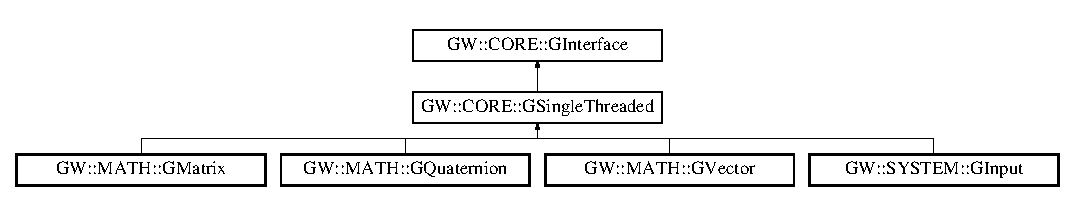
\includegraphics[height=2.270270cm]{class_g_w_1_1_c_o_r_e_1_1_g_single_threaded}
\end{center}
\end{figure}
\subsection*{Additional Inherited Members}


\subsection{Detailed Description}
This interface is only used to label and query interfaces which are not designed internally to support thread safety. 

The documentation for this class was generated from the following file\+:\begin{DoxyCompactItemize}
\item 
C\+:/\+Users/\+Devin Wright/\+Documents/\+Gate\+Ware\+Repo/gateware.\+git.\+0/\+Interface/\+G\+\_\+\+Core/G\+Single\+Threaded.\+h\end{DoxyCompactItemize}

\hypertarget{struct_g_w_1_1_g_u_u_i_i_d}{}\section{GW\+:\+:G\+U\+U\+I\+ID Struct Reference}
\label{struct_g_w_1_1_g_u_u_i_i_d}\index{G\+W\+::\+G\+U\+U\+I\+ID@{G\+W\+::\+G\+U\+U\+I\+ID}}


Gateware Universally Unique Interface I\+Dentifier.  




{\ttfamily \#include $<$G\+Defines.\+h$>$}

\subsection*{Public Member Functions}
\begin{DoxyCompactItemize}
\item 
\mbox{\Hypertarget{struct_g_w_1_1_g_u_u_i_i_d_a91cfd5559e56d01dd58d0d60f1704bd6}\label{struct_g_w_1_1_g_u_u_i_i_d_a91cfd5559e56d01dd58d0d60f1704bd6}} 
bool \mbox{\hyperlink{struct_g_w_1_1_g_u_u_i_i_d_a91cfd5559e56d01dd58d0d60f1704bd6}{operator==}} (const \mbox{\hyperlink{struct_g_w_1_1_g_u_u_i_i_d}{G\+U\+U\+I\+ID}} \&\+\_\+cmp) const
\begin{DoxyCompactList}\small\item\em Comparison operator overload. \end{DoxyCompactList}\end{DoxyCompactItemize}
\subsection*{Public Attributes}
\begin{DoxyCompactItemize}
\item 
\mbox{\Hypertarget{struct_g_w_1_1_g_u_u_i_i_d_aa51f004bf72e52a4e15b7568b9a7ec50}\label{struct_g_w_1_1_g_u_u_i_i_d_aa51f004bf72e52a4e15b7568b9a7ec50}} 
\begin{tabbing}
xx\=xx\=xx\=xx\=xx\=xx\=xx\=xx\=xx\=\kill
union \{\\
\mbox{\Hypertarget{union_g_w_1_1_g_u_u_i_i_d_1_1_0D0_a408b2437c2ea63a4cb75888db0ac62fb}\label{union_g_w_1_1_g_u_u_i_i_d_1_1_0D0_a408b2437c2ea63a4cb75888db0ac62fb}} 
\>struct \{\\
\>\>unsigned int {\bfseries byte4}\\
\>\>unsigned short {\bfseries byte2a}\\
\>\>unsigned short {\bfseries byte2b}\\
\>\>unsigned char {\bfseries byte8} \mbox{[}8\mbox{]}\\
\>\} \\
\>unsigned long long {\bfseries parts} \mbox{[}2\mbox{]}\\
\}; \\

\end{tabbing}\end{DoxyCompactItemize}


\subsection{Detailed Description}
Gateware Universally Unique Interface I\+Dentifier. 

Each \mbox{\hyperlink{struct_g_w_1_1_g_u_u_i_i_d}{G\+U\+U\+I\+ID}} defines a unique 128bit number identifying a particular version of an interface. This allows interfaces to be upgraded down the line safely without breaking legacy code. 

The documentation for this struct was generated from the following file\+:\begin{DoxyCompactItemize}
\item 
C\+:/\+Users/\+Devin Wright/\+Documents/\+Gate\+Ware\+Repo/gateware.\+git.\+0/\+Interface/\+G\+\_\+\+Core/G\+Defines.\+h\end{DoxyCompactItemize}

\hypertarget{struct_g_w_1_1_c_o_r_e_1_1_l_i_n_u_x___w_i_n_d_o_w}{}\section{GW\+:\+:C\+O\+RE\+:\+:L\+I\+N\+U\+X\+\_\+\+W\+I\+N\+D\+OW Struct Reference}
\label{struct_g_w_1_1_c_o_r_e_1_1_l_i_n_u_x___w_i_n_d_o_w}\index{G\+W\+::\+C\+O\+R\+E\+::\+L\+I\+N\+U\+X\+\_\+\+W\+I\+N\+D\+OW@{G\+W\+::\+C\+O\+R\+E\+::\+L\+I\+N\+U\+X\+\_\+\+W\+I\+N\+D\+OW}}


The structure used to pass into Input libraries on Linux.  




{\ttfamily \#include $<$G\+Key\+Defines.\+h$>$}

\subsection*{Public Attributes}
\begin{DoxyCompactItemize}
\item 
\hypertarget{struct_g_w_1_1_c_o_r_e_1_1_l_i_n_u_x___w_i_n_d_o_w_a51fadcfa59276c1c0ab7fdc6af733f4f}{}\label{struct_g_w_1_1_c_o_r_e_1_1_l_i_n_u_x___w_i_n_d_o_w_a51fadcfa59276c1c0ab7fdc6af733f4f} 
void $\ast$ {\bfseries \+\_\+\+Window}
\item 
\hypertarget{struct_g_w_1_1_c_o_r_e_1_1_l_i_n_u_x___w_i_n_d_o_w_a1b1d6b2b7b133fc54f67dcce4c2f1ed5}{}\label{struct_g_w_1_1_c_o_r_e_1_1_l_i_n_u_x___w_i_n_d_o_w_a1b1d6b2b7b133fc54f67dcce4c2f1ed5} 
void $\ast$ {\bfseries \+\_\+\+Display}
\end{DoxyCompactItemize}


The documentation for this struct was generated from the following file\+:\begin{DoxyCompactItemize}
\item 
G\+Key\+Defines.\+h\end{DoxyCompactItemize}

%--- End generated contents ---

% Index
\backmatter
\newpage
\phantomsection
\clearemptydoublepage
\addcontentsline{toc}{chapter}{Index}
\printindex

\end{document}
